\documentclass[12pt, compress]{beamer}

\usetheme{m}

\usepackage{booktabs}
\usepackage[scale=2]{ccicons}
\usepackage{minted}
\usepackage{tikz}
\usetikzlibrary{intersections}
\usepackage{pgfplots}
\usepackage{standalone}
\usepackage{array}
\usepackage[percent]{overpic}
\usepackage[font=footnotesize]{caption}
%\usepackage{subfigure}
\usepackage{caption}
\usepackage{subcaption}
\usepackage{graphicx}

% Math packages
\usepackage{amsthm}
\usepackage{amssymb}
\usepackage{mathtools}
\usepackage{amsfonts}
\usepackage{amsmath}
\usepackage{kbordermatrix}
\usepackage{blkarray}

% Bibliography
\usepackage{natbib}
\bibpunct{[}{]}{,}{a}{}{;}


% For presentation mode
%\usepackage{pgfpages}
%\setbeameroption{show notes}
%\setbeameroption{show notes on second screen=right}

% Numbered sections in table of contents
\setbeamertemplate{section in toc}[sections numbered]
\setbeamertemplate{frametitle continuation}[from second]

\usemintedstyle{trac}

\title{Attenuation-based Light Field Displays}
\subtitle{Bachelor Thesis}
\date{June 3, 2016}
\author{Adrian W\"alchli}
\institute{Institut f\"ur Informatik und angewandte Mathematik}

\begin{document}

\setlength{\leftmargini}{0pt}
\setlength{\fboxsep}{0pt}%

\maketitle

\begin{frame}[fragile]
	\frametitle{Outline}
	\tableofcontents
\end{frame}

\section{Introduction}

\begin{frame}[fragile]
	\frametitle{Existing 3D Displays}
	
	\begin{figure}
		\captionsetup[sub]{font=scriptsize}
		\subcaptionbox*{\cite{360_display}}
		{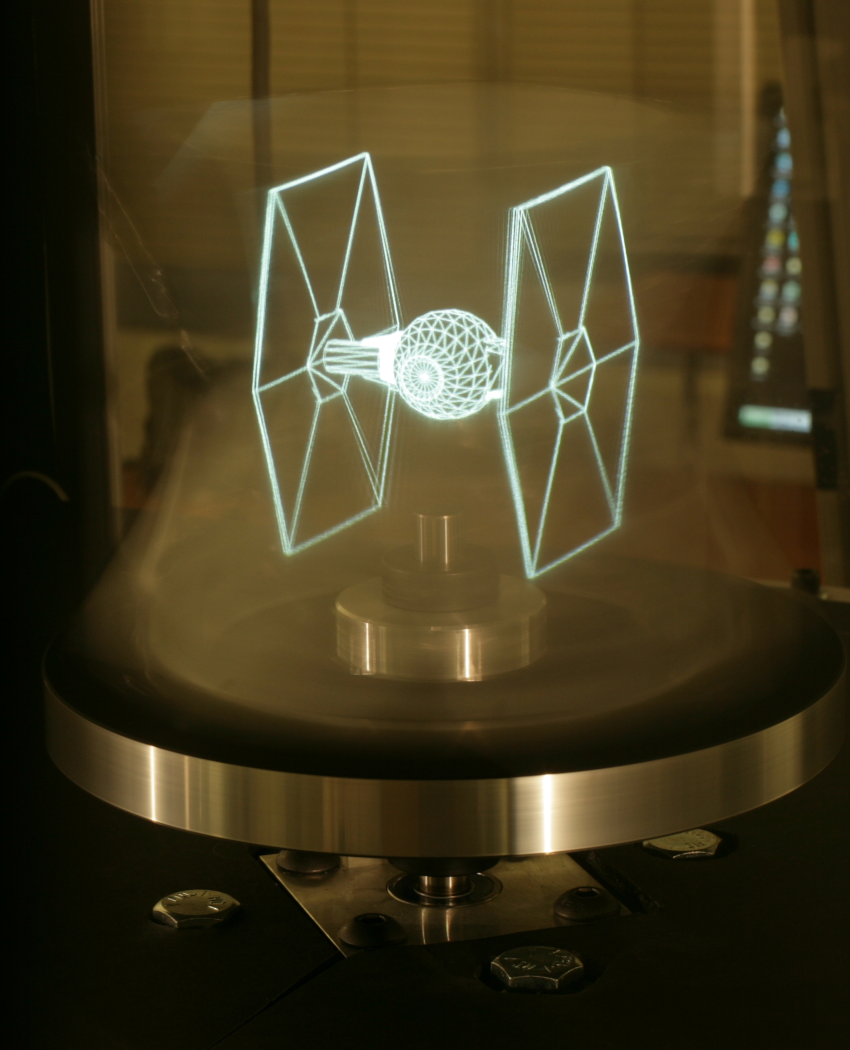
\includegraphics[height=6.5cm]{figures/overview_displays/360_deg_display}}
		\hspace{0.4cm}
		\subcaptionbox*{\href{https://en.wikipedia.org/wiki/Autostereoscopy}{en.wikipedia.org/wiki/Autostereoscopy}}
		{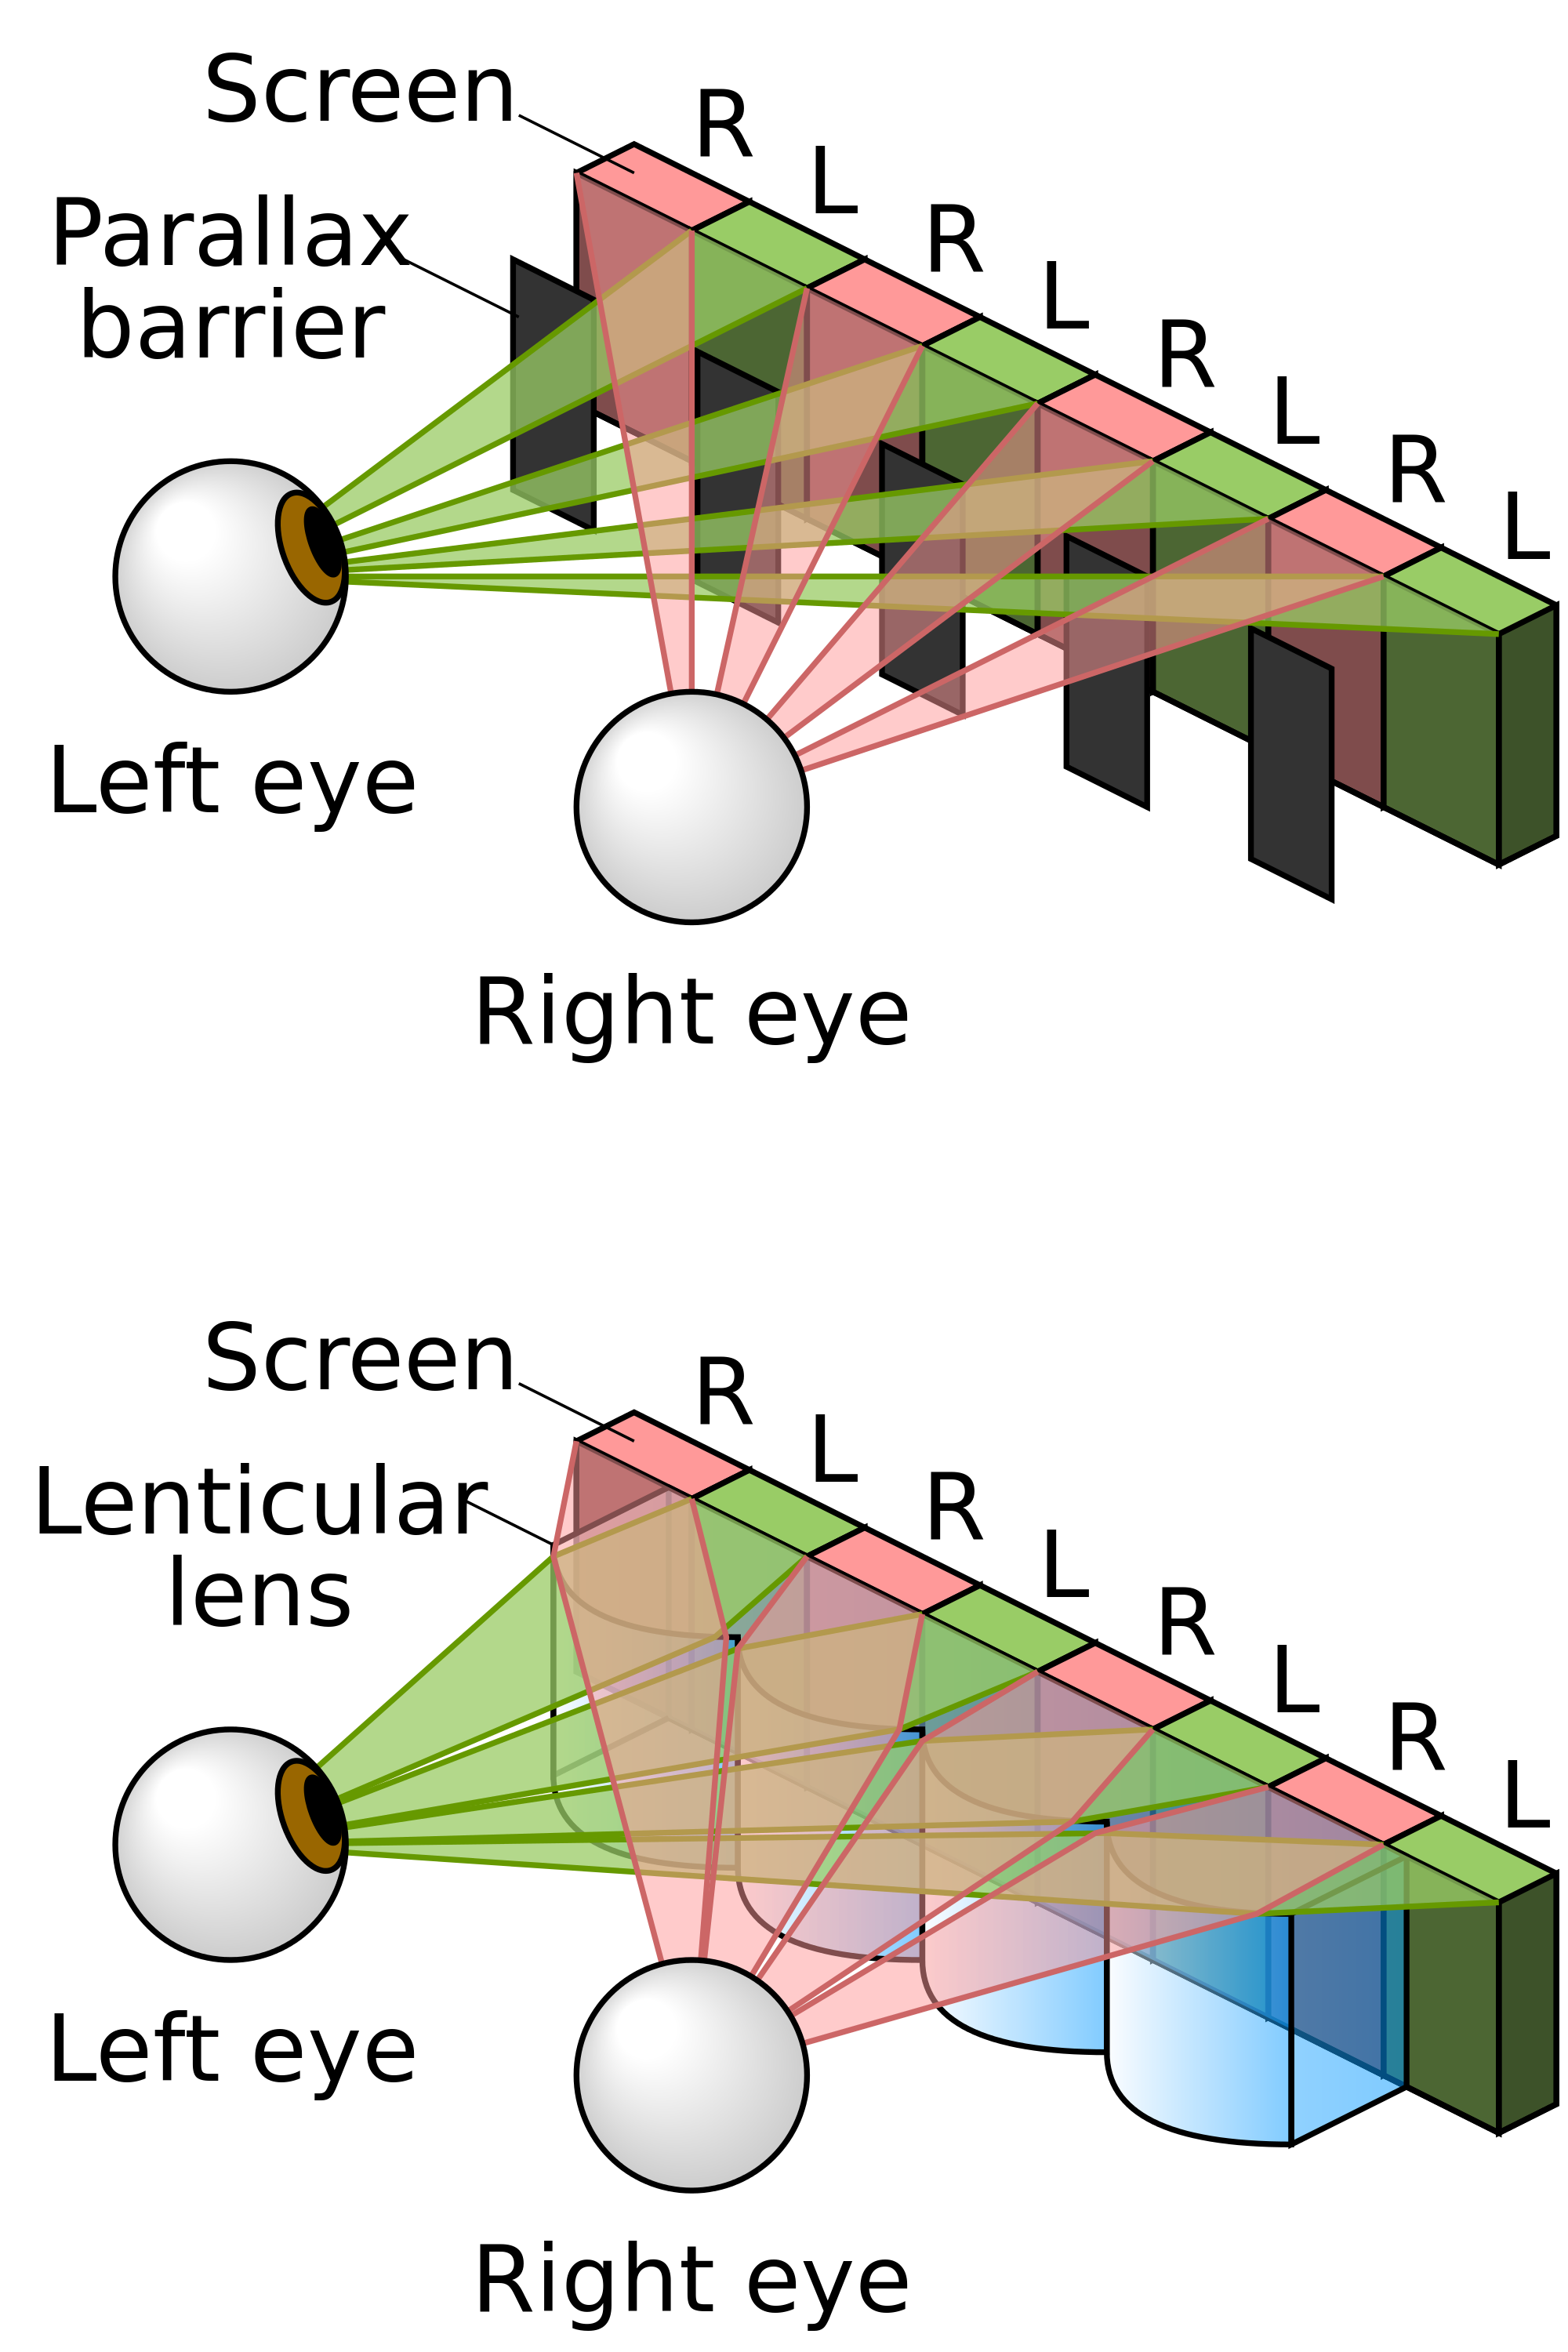
\includegraphics[height=6.5cm]{figures/overview_displays/parallax_barrier_vs_lenticular}}	
	\end{figure}
\end{frame}

\begin{frame}[fragile]
	\frametitle<1>{Glasses}
	\frametitle<2>{Glasses-free}
	
	\begin{figure}
		\includegraphics<1>[width=5cm]{figures/overview_displays/3d_glasses}
		\includegraphics<2>[width=5cm]{figures/overview_displays/no_3d_glasses}
	\end{figure}

\end{frame}

\begin{frame}[fragile]
	\frametitle{Today}
	
	\begin{figure}
		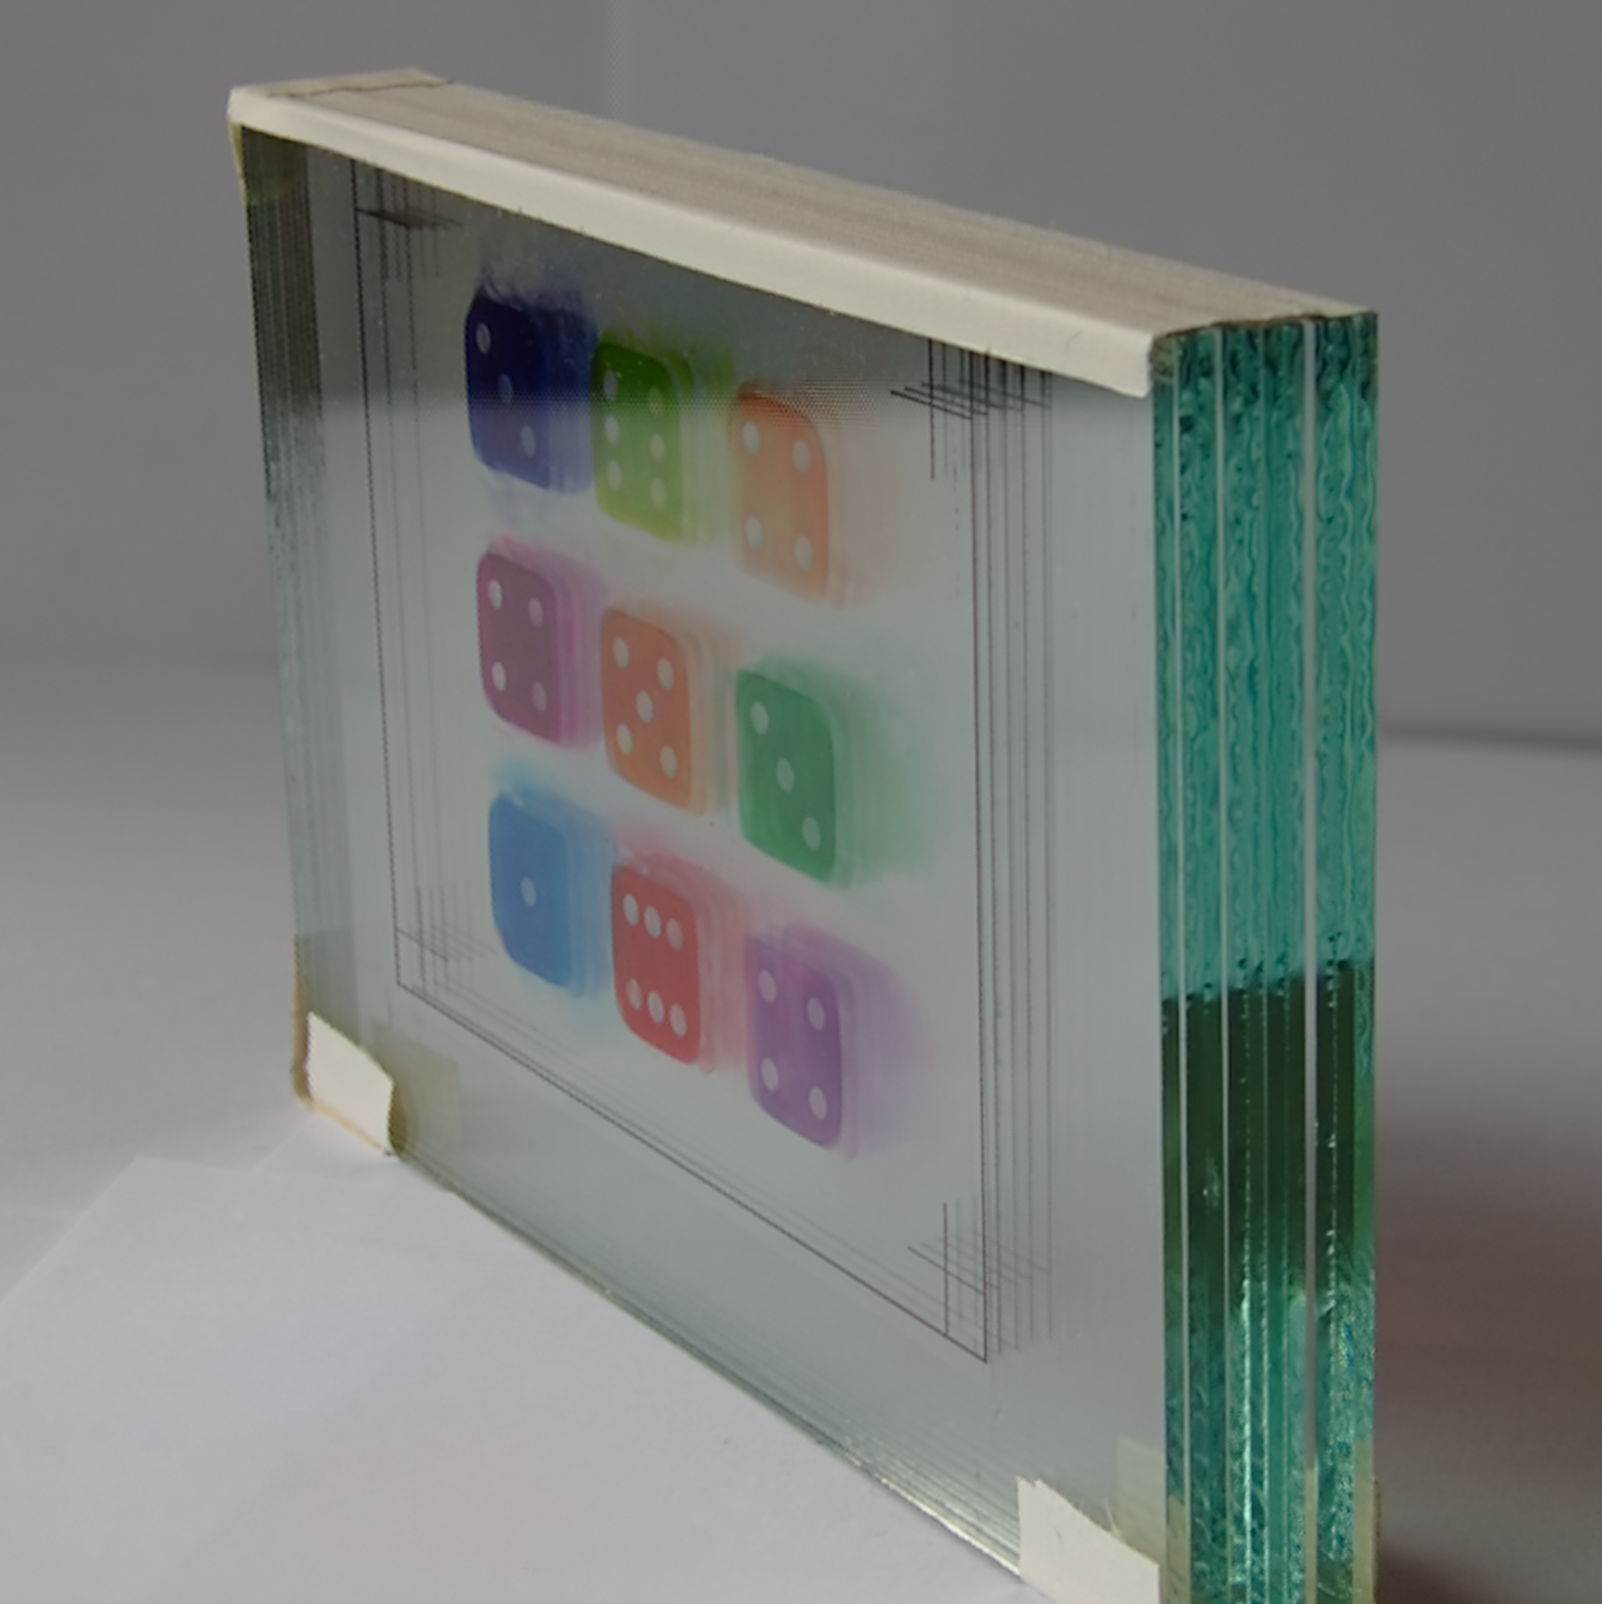
\includegraphics[height=7cm]{images/glass_plates_front_view_cropped}
	\end{figure}
\end{frame}

\begin{frame}[fragile]
	\frametitle{Layered 3D}

	\begin{columns}[onlytextwidth]
		\column{0.5\textwidth}
			\begin{block}{}
				Layered 3D: Tomographic Image Synthesis for Attenuation-based Light Field and High Dynamic Range Displays
			\end{block}
			\begin{block}{}
				\cite{WetzsteinTomo}
			\end{block}
		\column{0.5\textwidth}
			\begin{figure}
				\fbox{
					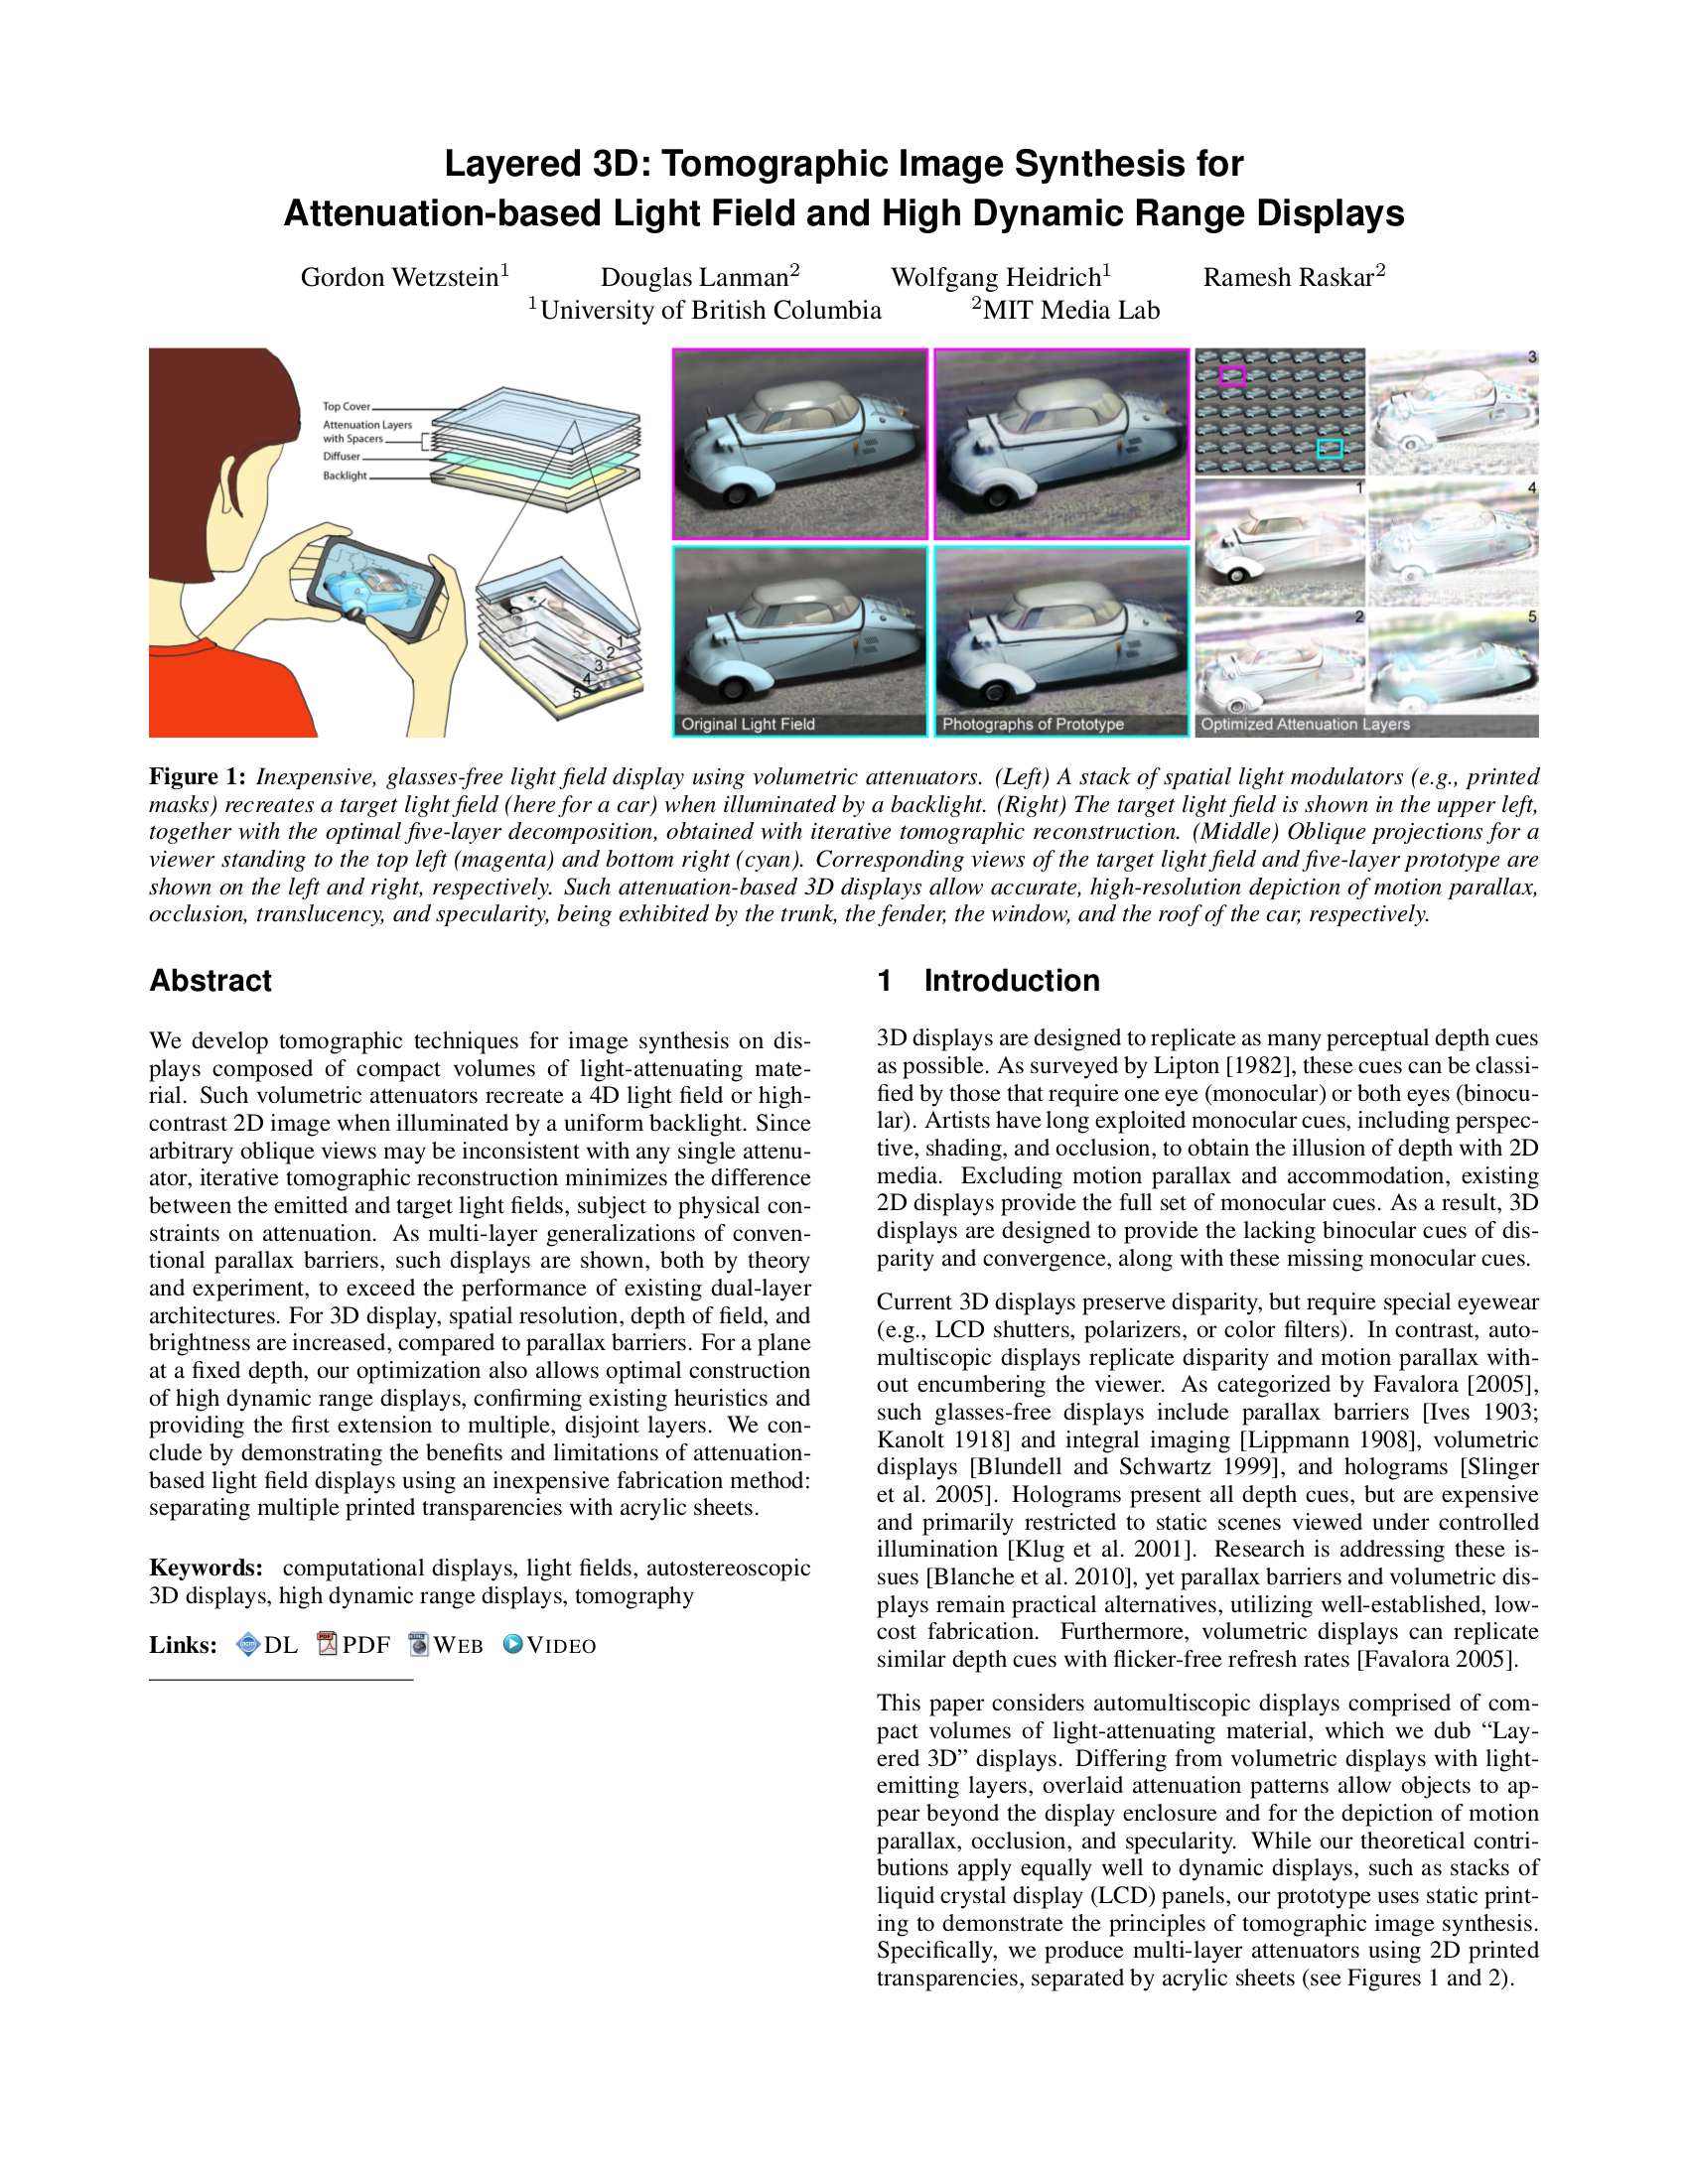
\includegraphics[height=7cm]{images/Layered_3D_paper_front_page.png}
				}
			\end{figure}
	\end{columns}
	
\end{frame}

\section{Light Fields}

\begin{frame}[fragile]
	\frametitle{The Plenoptic Function}
	
	\begin{columns}[onlytextwidth]
		\column{0.6\textwidth}
			\begin{itemize}
				\item \alert<1>{Measures light in the world}
				\item \alert<2>{$P(x, y, z, \theta, \phi, t, \lambda)$}
				\begin{itemize}
					\item \alert<3>{Position} %$(x, y, z)$
					\item \alert<4>{Viewing direction} %$(\theta, \phi)$
					\item \alert<5>{Time} %$t$
					\item \alert<6>{Wavelength} %$\lambda$
				\end{itemize}
				\item \alert<7>{Reduce dimensions of $P$}
			\end{itemize}
		\column{0.4\textwidth}
			\begin{figure}
				\captionsetup{font=scriptsize}
				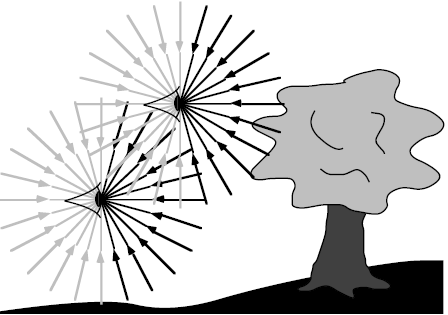
\includegraphics[width = 4cm]{images/plenoptic.png}
				\caption*{\cite{AdelsonBergen}}
			\end{figure}
	\end{columns}
	
\end{frame}

\begin{frame}[fragile]
	\frametitle{The 4D Light Field}
	
	\begin{itemize}
		\item $L(u, v, s, t)$
		\item Defined by two planes
	\end{itemize}
	\begin{center}
		\documentclass{standalone}
\usepackage{tikz}

\begin{document}
	
	\begin{tikzpicture}[scale = 0.4]
	
		\filldraw[draw = black, fill = white] (0, 0) -- (5, -2) -- (5, 5) -- (0, 7) -- cycle;
		\filldraw[draw = black, fill = white] (9, 3) -- (14, 1) -- (14, 8) -- (9, 10) -- cycle;
		
		\draw[<-] (-3, 4) -- (1, 4);
		\draw (5, 4) -- (11, 4);
		\draw (14, 4) -- (17, 4);
		
		\node [left] at (-3, 4) {$L(u, v, s, t)$};
		
		
		\draw[fill] (1, 4) circle [radius = 0.1];
		\draw[fill] (11, 4) circle [radius = 0.1];
		
		\node[below right] at (1, 4) {$(u, v)$};
		\node[below right] at (11, 4) {$(s, t)$};
	
	\end{tikzpicture}
	
\end{document}
	\end{center}
\end{frame}

\begin{frame}[fragile]
	\frametitle{Light Field Acquisition}
	
	\begin{figure}
		\captionsetup{font=scriptsize}
		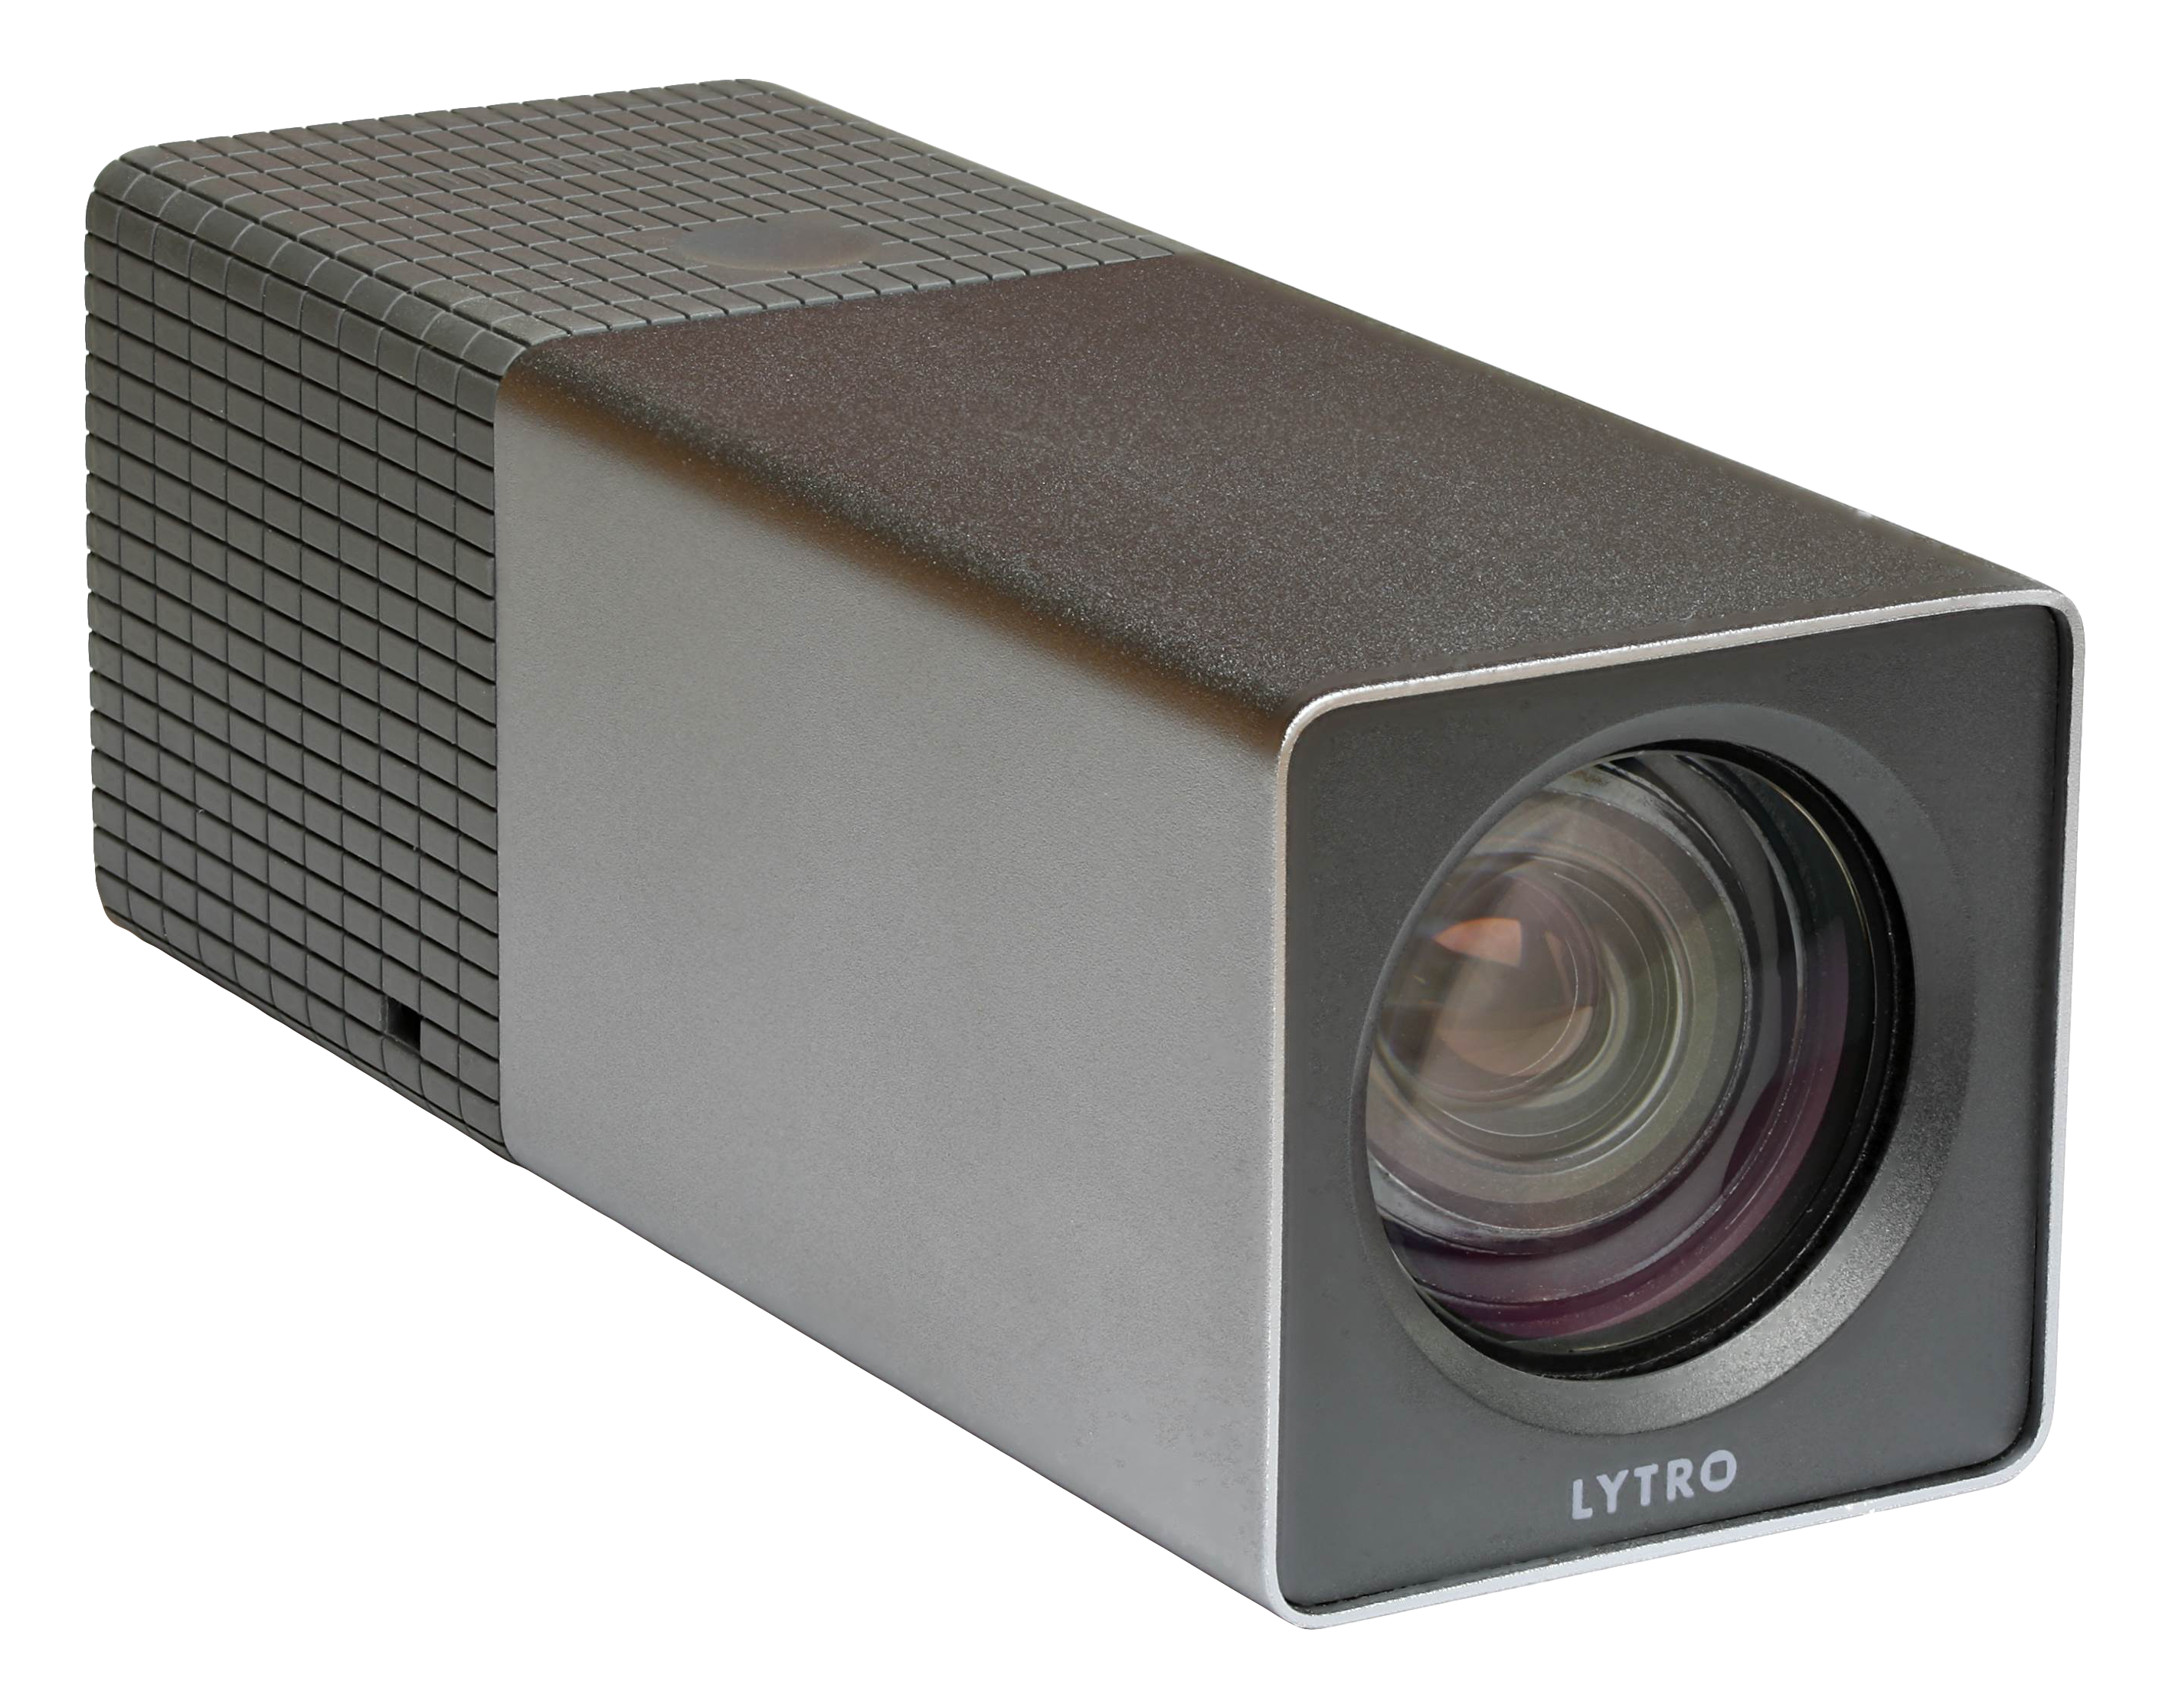
\includegraphics[height = 6cm]{images/Lytro_Light_Field_Camera-front_background_removed.png}
		\caption*{Lytro plenoptic camera. Source: \href{https://de.wikipedia.org/wiki/Lytro}{de.wikipedia.org/wiki/Lytro}}
	\end{figure}
	
\end{frame}

\begin{frame}[fragile]
	\frametitle{Light Field Acquisition}
	
	\begin{figure}
		\captionsetup{font=scriptsize}
		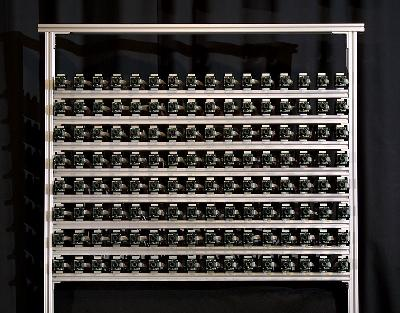
\includegraphics[height = 6cm]{images/stanford_camera_array_2.jpg}
		\caption*{Stanford camera array. Source: \href{http://lightfield.stanford.edu}{lightfield.stanford.edu}}
	\end{figure}
	
\end{frame}

\begin{frame}[fragile]
	\frametitle{Light Field Acquisition}
	
	\begin{figure}
		\captionsetup{font=scriptsize}
		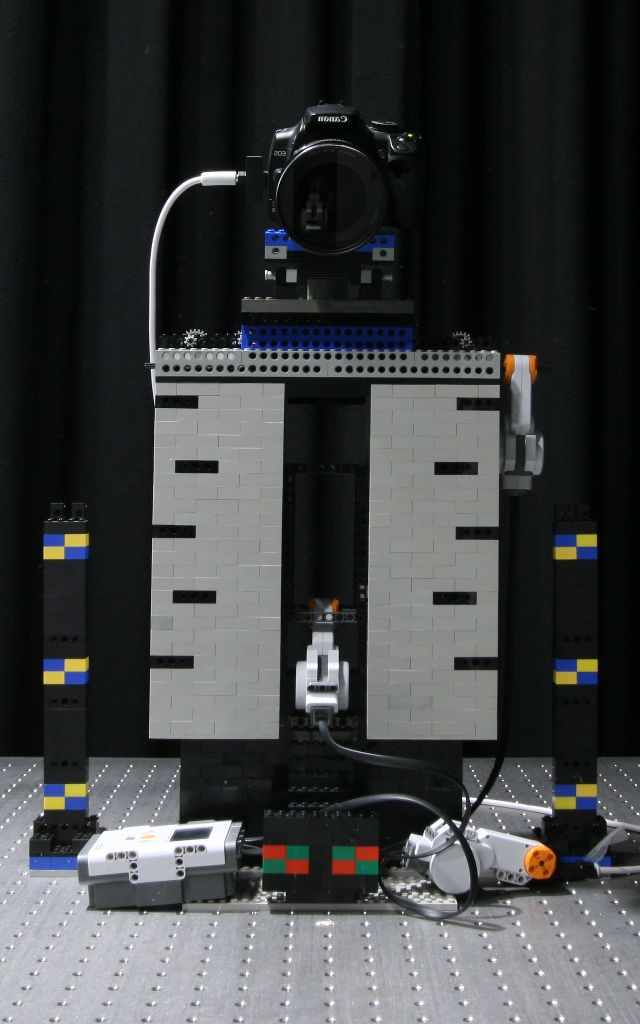
\includegraphics[height = 6cm]{images/lego_camera_gantry}
		\caption*{Lego gantry. Source: \href{http://lightfield.stanford.edu}{lightfield.stanford.edu}}
	\end{figure}
	
\end{frame}

\section{Attenuation Display}

\begin{frame}[fragile]
	\frametitle{The Beer-Lambert Law}
	\begin{figure}
		\centering
		\includegraphics<1>[height = 7cm]{figures/beer-lambert/lambert-beer-law_illustration.pdf}
		\includegraphics<2>[height = 7cm]{figures/beer-lambert/lambert-beer-law_layers1.pdf}
		\includegraphics<3>[height = 7cm]{figures/beer-lambert/lambert-beer-law_layers2.pdf}
		\includegraphics<4>[height = 7cm]{figures/beer-lambert/lambert-beer-law_layers3.pdf}
	\end{figure}
\end{frame}

\begin{frame}[fragile]
	\frametitle{Display Architecture}
	
	\begin{figure}
		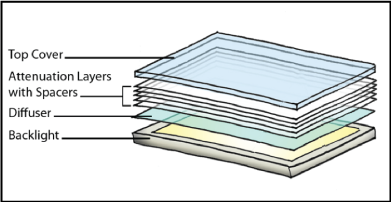
\includegraphics[width=10cm]{images/display_architecture.png}
		\caption*{\cite{WetzsteinTomo}}	
	\end{figure}
\end{frame}

\begin{frame}[fragile]
	\frametitle{Problem Statement}
	{\large
	\begin{block}{Given a light field}
		Produce layers that attenuate light from backlight such that display creates the given light field
	\end{block}
	}
\end{frame}

\begin{frame}[fragile]
	\frametitle{Light Transmission}
	\vspace{1cm}
	\begin{columns}[onlytextwidth]
		\column{0.45\textwidth} 
			\documentclass{standalone}
\usepackage{tikz}
\usepackage{xcolor}
\usetikzlibrary{intersections}

\begin{document}
	
	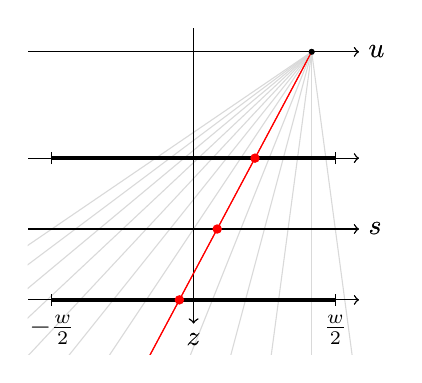
\begin{tikzpicture}[scale = 0.15,
						one end extended/.style = {shorten <= -#1},
	 					one end extended/.default = 1cm,
	 					]
	
		\colorlet{lightgray}{gray!30}
		
		% Top and bottom layer planes
		\draw[->, name path = bottomLayer] (-14, -6) -- (14, -6);
		\draw[->, name path = topLayer] (-14, 6) -- (14, 6);
					
		% Camera plane
		\draw[->] (-14, 15) -- (14, 15);
		\node[right] at (14, 15) {$u$};
		
		% Sensor plane
		\draw[<-, name path = sensor] (14, 0) -- (-14, 0);
		\node[right] at (14, 0) {$s$};
			
		% Camera position marker
		\coordinate (cameraCenter) at (10, 15);
		\fill[black] (cameraCenter) circle[radius = 0.25];
				
		\draw[ultra thick] (-12, -6) -- (12, -6);
		\draw[ultra thick] (-12, 6) -- (12, 6);
				
		% z-axis
		\draw[->] (0, 15 + 2) -- (0, -8);
		\node[below] at (0, -8) {$z$};
		
		% Save current bounding box to clip light rays
		\coordinate (NE) at (current bounding box.north east);
		\coordinate (SW) at (current bounding box.south west);
		\clip (SW) rectangle (NE);
		
		% Rays and intersections
		\coordinate (s0) at (-12, 0);
		\coordinate (s1) at (-10, 0);
		\coordinate (s2) at (-8, 0);
		\coordinate (s3) at (-6, 0);
		\coordinate (s4) at (-4, 0);
		\coordinate (s5) at (-2, 0);
		\coordinate (s6) at (0, 0);
		\coordinate (s7) at (2, 0);
		\coordinate (s8) at (4, 0);
		\coordinate (s9) at (6, 0);
		\coordinate (s10) at (8, 0);
		\coordinate (s11) at (10, 0);
		\coordinate (s12) at (12, 0);
		
		\draw[one end extended = 10cm, lightgray] (s0) -- (cameraCenter);
		\draw[one end extended = 10cm, lightgray] (s1) -- (cameraCenter);
		\draw[one end extended = 10cm, lightgray] (s2) -- (cameraCenter);
		\draw[one end extended = 10cm, lightgray] (s3) -- (cameraCenter);
		\draw[one end extended = 10cm, lightgray] (s4) -- (cameraCenter);
		\draw[one end extended = 10cm, lightgray] (s5) -- (cameraCenter);
		\draw[one end extended = 10cm, lightgray] (s6) -- (cameraCenter);
		\draw[one end extended = 10cm, red, name path = ray] (s7) -- (cameraCenter);
		\draw[one end extended = 10cm, lightgray] (s8) -- (cameraCenter);
		\draw[one end extended = 10cm, lightgray] (s9) -- (cameraCenter);
		\draw[one end extended = 10cm, lightgray] (s10) -- (cameraCenter);
		\draw[one end extended = 10cm, lightgray] (s11) -- (cameraCenter);
		\draw[one end extended = 10cm, lightgray] (s12) -- (cameraCenter);
		
		% Draw lines of coordinate system again on top of rays
		\draw[->] (-14, -6) -- (14, -6);
		\draw[->] (-14, 6) -- (14, 6);
		\draw[->] (-14, 15) -- (14, 15);
		\node[right] at (14, 15) {$u$};
		\draw[<-] (14, 0) -- (-14, 0);
		\node[right] at (14, 0) {$s$};
		\draw[ultra thick] (-12, -6) -- (12, -6);
		\draw[ultra thick] (-12, 6) -- (12, 6);
		\draw[->] (0, 15 + 2) -- (0, -8);
		\node[below] at (0, -8) {$z$};
		
		\draw[one end extended = 10cm, red, name path = ray] (s7) -- (cameraCenter);
		\fill[black] (cameraCenter) circle[radius = 0.25];
		
		% Intersection markers
		\fill[red] (-1.2, -6) circle[radius = 0.4];
		\fill[red] (2, 0) circle[radius = 0.4];
		\fill[red] (5.2, 6) circle[radius = 0.4];
							
		% Width markers
		\draw (-12, -0.5 + 6) -- (-12, 0.5 + 6);
		\draw (12, -0.5 + 6) -- (12, 0.5 + 6);
		\draw (-12, -0.5 - 6) -- (-12, 0.5 - 6);
		\draw (12, -0.5 - 6) -- (12, 0.5 - 6);
		\node[below] at (-12, -0.5 - 6) {$-\frac{w}{2}$};
		\node[below] at (12, -0.5 - 6) {$\frac{w}{2}$};
		
	\end{tikzpicture}
	
\end{document}
		\column{0.4\textwidth}
			\begin{equation*}
				L_m = L_0 \prod_{n=1}^{N} t^{(n)} (h(m, n)) 
			\end{equation*}
			\begin{itemize}[<alert@+>]
			    \item[$L_m$] Color of ray $m$
			    \item[$t$] Transmission
			    \item[$h$] Intersection 
			\end{itemize}
	\end{columns}
	\vspace{1cm}
	\begin{center}
		\visible<4>{\alert{From now on: $L_0 = 1$}}
	\end{center}
\end{frame}

\begin{frame}[fragile]
	\frametitle{From Transmission to Absorbance}
	
	\begin{itemize}[<+- | alert@+>]
		\item Transmission values unknown
		\item Solve equations simultaneously for all rays
		\item This is hard
		\item Transform to log-domain
		\item Solve for absorbance
	\end{itemize}
	\visible<1,2,3,4,5>{
	\begin{equation*}
		L_m = \prod_{n=1}^{N} t^{(n)} (h(m, n)) 
	\end{equation*}}
	\visible<4,5>{
	\begin{center}
		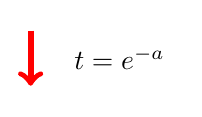
\begin{tikzpicture}
			\draw[->, red, line width = 0.075cm] (0, 0) -- (0, -0.7) node[midway, right, xshift=0.4cm, black] {$t = e^{-a}$};
		\end{tikzpicture}
	\end{center}
	\begin{equation*}
		\text{log}(L_m) = - \sum_{n=1}^{N} a^{(n)} (h(m, n)) 
	\end{equation*}}
	
\end{frame}

\begin{frame}[fragile]
	\frametitle{Ray Casting}
	
	\begin{itemize}[<alert@+>]
		\item One linear constraint per ray
		\item Create a big matrix $P$
		\item Matrix encodes intersections
	\end{itemize}
	\vspace{2cm}
	\begin{equation*}
			\text{log}(L_m) = -\sum_{n=1}^{N} a^{(n)} (h(m, n)) 
	\end{equation*}
	
\end{frame}

\begin{frame}[fragile]
	\frametitle{The Equation}
	
	{\LARGE
		\begin{equation*}
			\text{log}(L) = - P \alpha
		\end{equation*}
	}
	\begin{itemize} %[<alert@+>]
		\item $L$ Vectorized light field
		\item $\alpha$ Vector holding unkowns
	\end{itemize}
\end{frame}

\begin{frame}[fragile]
	\frametitle{Optimization Problem}
	
	\begin{equation*}
		\begin{aligned}
			& \underset{\alpha}{\text{argmin}} 	& & \left\lVert P \alpha + \log(L) \right\rVert ^2 \\
			& \text{subject to} 				& & \alpha \geq 0.
		\end{aligned}
	\end{equation*}
	
	\begin{itemize}
		\item Proposed by \cite{WetzsteinTomo}
		\item System is overdetermined
%			\begin{itemize}
%				\item More equations than unknowns
%			\end{itemize}
		\item Need iterative solver
		\item Negative absorption ($\alpha < 0$) is physically not possible
%		\item The theoretical model supports negative absorption
	\end{itemize}
\end{frame}

\begin{frame}[fragile]
	\frametitle{Example: Lego Truck}
	
	\begin{center}
		\begin{tabular}{cc}
			\raisebox{-.5\height}{
				\begin{overpic}[width=5cm,tics=10]{images/layers_and_projections/legotruck/1}
					\put (63, 60) {bottom}
				\end{overpic}
			} & 
			\raisebox{-.5\height}{
				\begin{overpic}[width=5cm,tics=10]{images/layers_and_projections/legotruck/2}
					\put (65, 60) {middle}
				\end{overpic}
			} 
			\\
			\raisebox{-.5\height}{
				\begin{overpic}[width=5cm,tics=10]{images/layers_and_projections/legotruck/3}
					\put (78, 60) {top}
				\end{overpic}
			} & 
			\begin{tabular}{@{}c@{}}
				$6 \times 6 \times 480 \times 640$ \\
				$\sim$ 2 minutes
			\end{tabular} 
		\end{tabular}
	\end{center}
\end{frame}

\begin{frame}[fragile]
	\frametitle{Example: Lego Truck}
	
	Goal: Simulate viewing experience before assembly
	\begin{equation*}
		I = e^{- P \alpha}
	\end{equation*}
	
	\begin{center}
		\begin{tabular}{c p{0cm} c}
			Original & & Simulation \\
			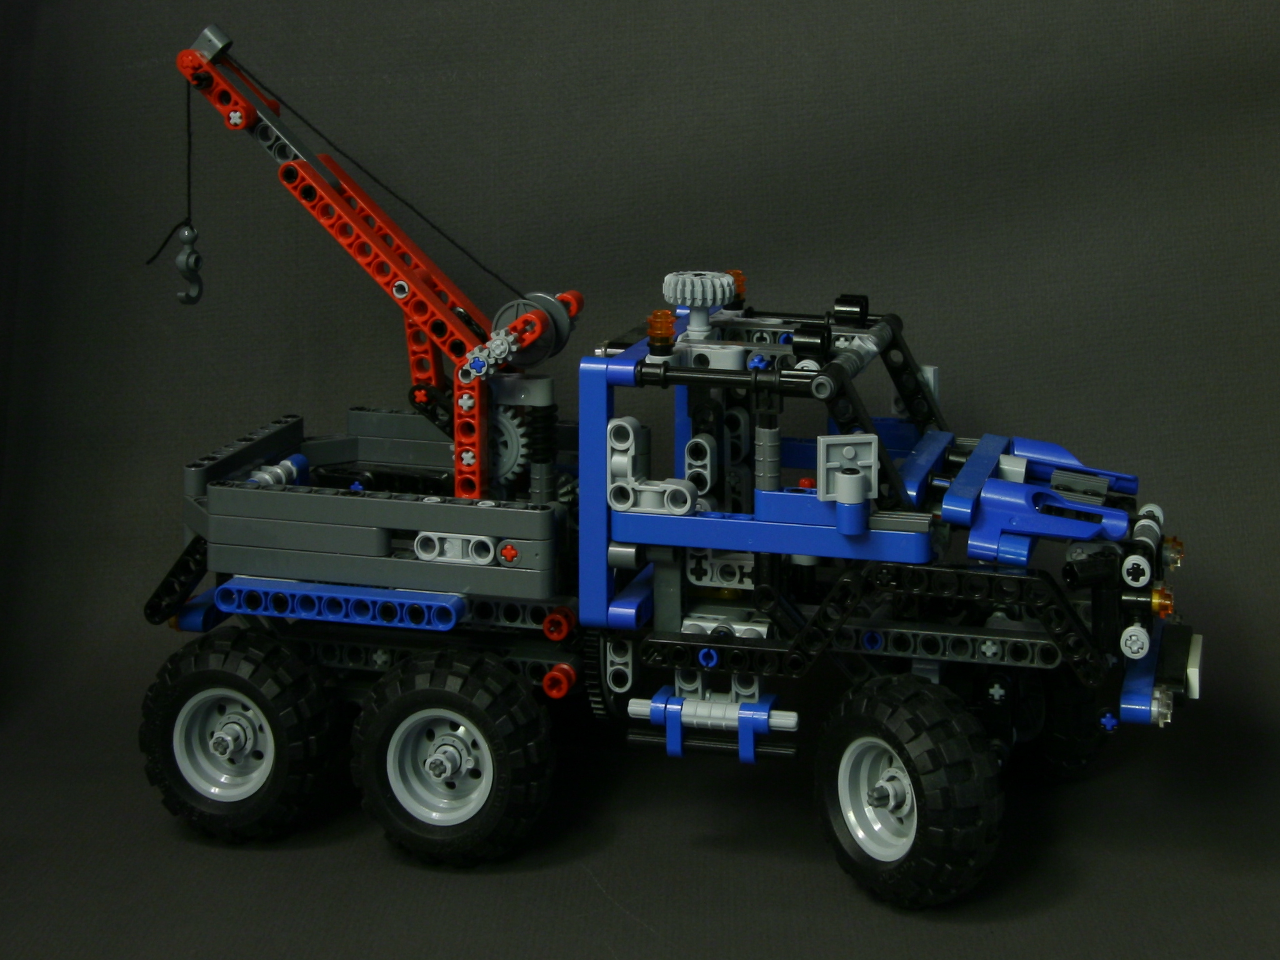
\includegraphics[width = 5cm]{images/layers_and_projections/legotruck/original/08_08}
			& & 
\includegraphics[width = 5cm]{images/layers_and_projections/legotruck/Reconstruction_of_view_(3,3)}
		\end{tabular}
	\end{center}
	{\scriptsize Light field courtesy: \href{http://lightfield.stanford.edu/lfs.html}{Stanford Light Field Archive}}

\end{frame}

\begin{frame}[fragile]
	\frametitle{Example: Lego Truck}
	\vspace{-0.5cm}
	\begin{center}
		\begin{tabular}{c p{0cm} c}
			\begin{tabular}{@{}c@{}}Original \\ $17 \times 17 \times 960 \times 1280$\end{tabular}
			& & \begin{tabular}{@{}c@{}}Simulation (3 Layers) \\ $6 \times 6 \times 480 \times 640$\end{tabular} \\
			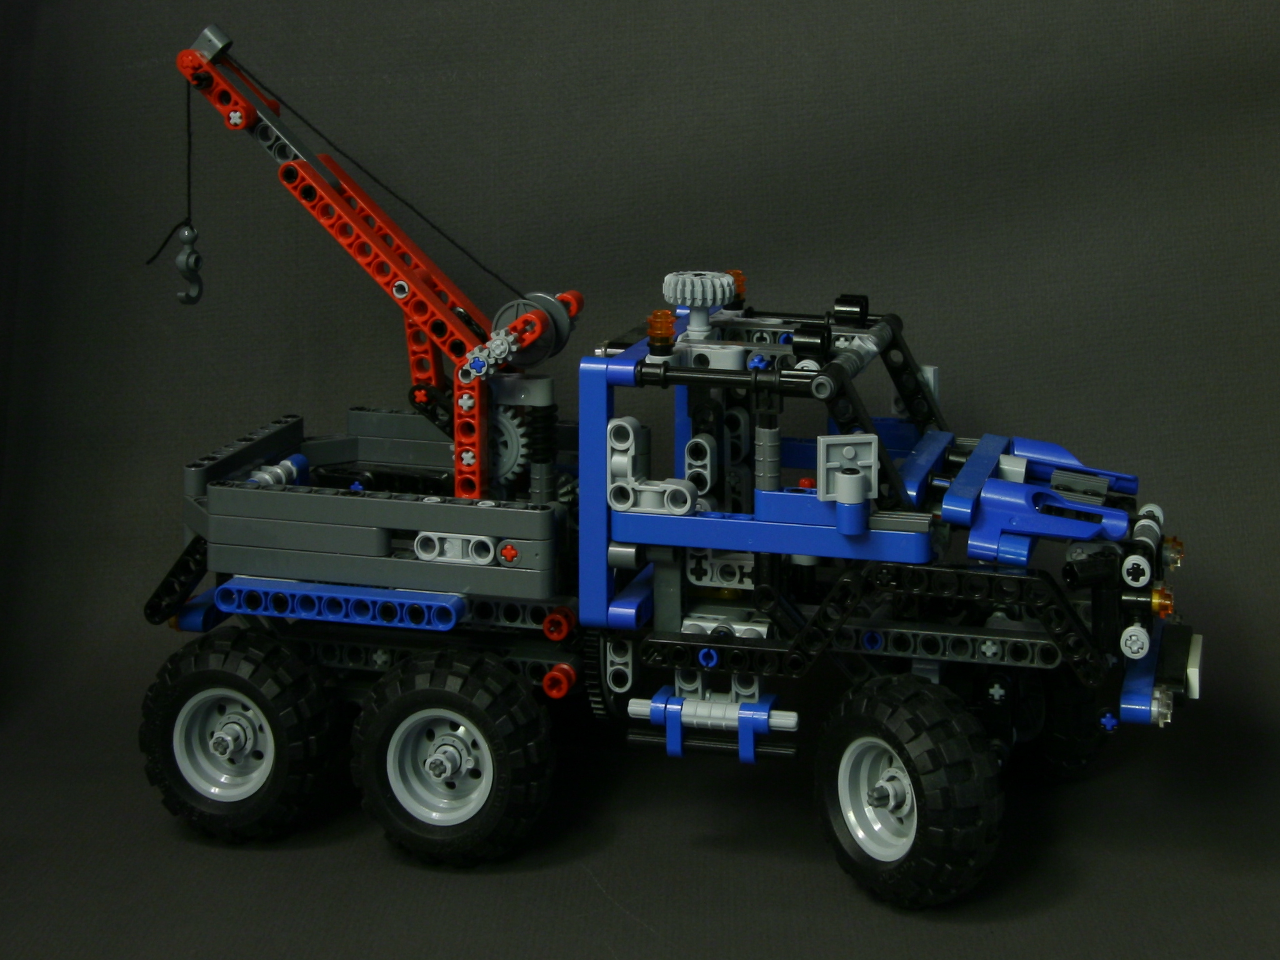
\includegraphics[width = 5cm, trim={4cm, 20cm, 30cm, 0}, clip]{images/layers_and_projections/legotruck/original/08_08}
			& & 
\includegraphics[width = 5cm, trim={2cm, 10cm, 15cm, 0}, clip]{figures/simulated_views/legotruck/3Layers_legotruck/Reconstruction_of_view_(3,3)}
		\end{tabular}
	\end{center}
\end{frame}

\begin{frame}[fragile]
	\frametitle{Example: Lego Truck}
	\vspace{-0.5cm}
	\begin{center}
		\begin{tabular}{c p{0cm} c}
			\begin{tabular}{@{}c@{}}Original \\ $17 \times 17 \times 960 \times 1280$\end{tabular}
			& & \begin{tabular}{@{}c@{}}Simulation (5 Layers) \\ $6 \times 6 \times 480 \times 640$\end{tabular} \\
			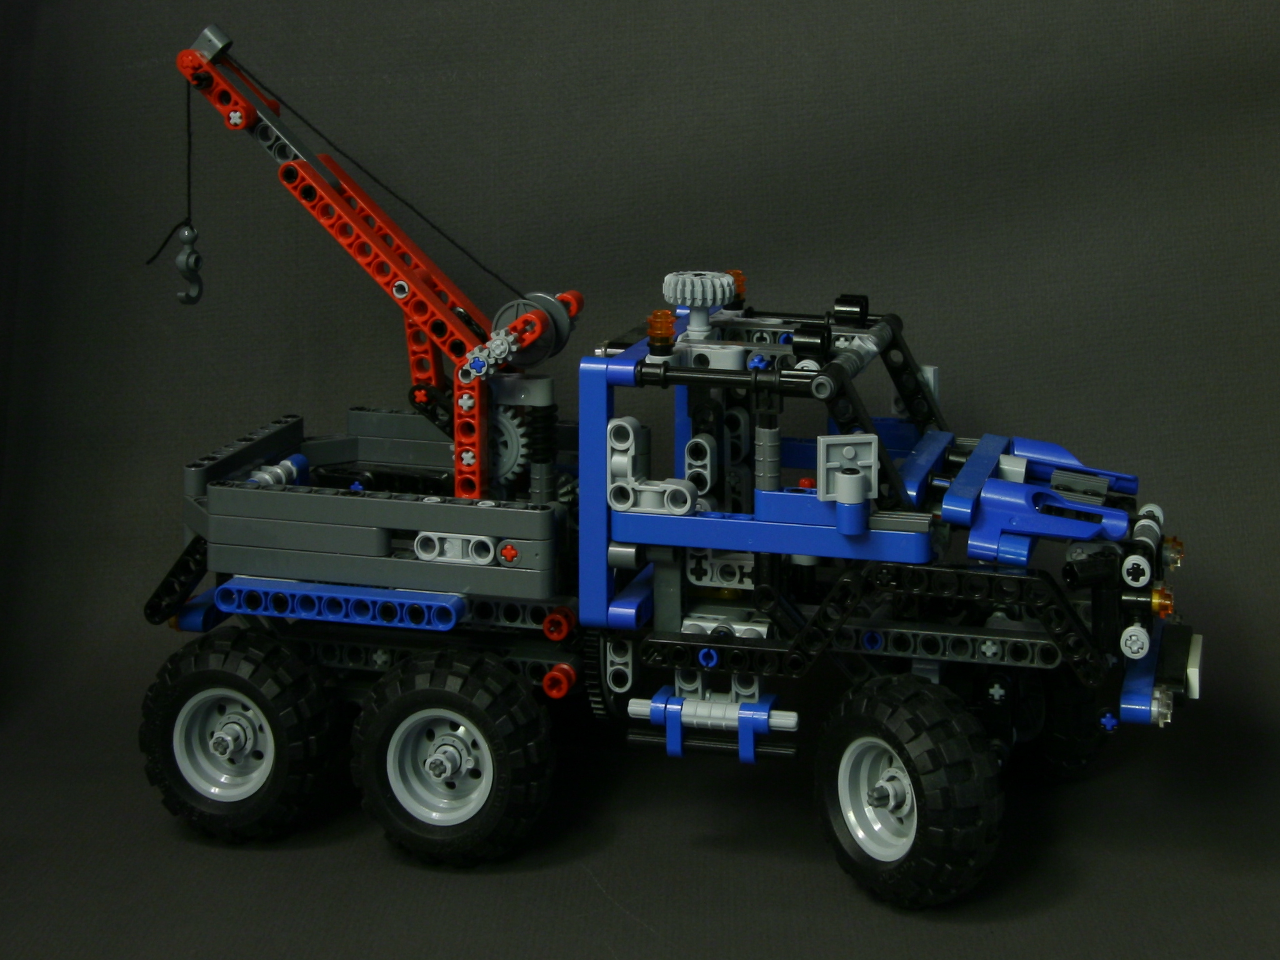
\includegraphics[width = 5cm, trim={4cm, 20cm, 30cm, 0}, clip]{images/layers_and_projections/legotruck/original/08_08}
			& & 
\includegraphics[width = 5cm, trim={2cm, 10cm, 15cm, 0}, clip]{figures/simulated_views/legotruck/5Layers_legotruck/Reconstruction_of_view_(3,3)}
		\end{tabular}
	\end{center}
\end{frame}

\begin{frame}[fragile]
	\frametitle{Example: Lego Truck}
	\vspace{-0.5cm}
	\begin{center}
		\begin{tabular}{c p{0cm} c}
			\begin{tabular}{@{}c@{}}Original \\ $17 \times 17 \times 960 \times 1280$\end{tabular}
			& & \begin{tabular}{@{}c@{}}Simulation (10 Layers) \\ $6 \times 6 \times 480 \times 640$\end{tabular} \\
			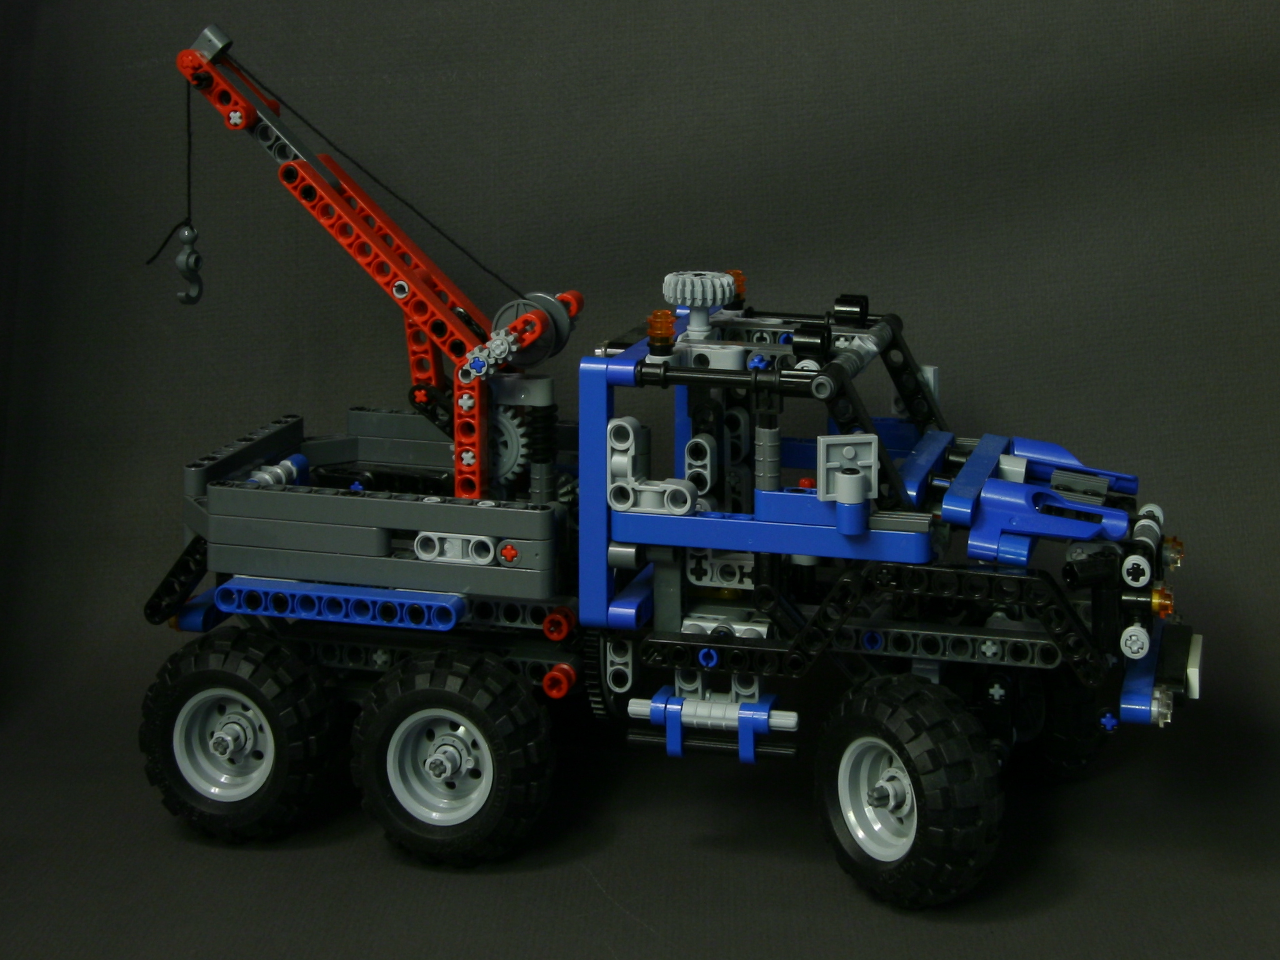
\includegraphics[width = 5cm, trim={4cm, 20cm, 30cm, 0}, clip]{images/layers_and_projections/legotruck/original/08_08}
			& & 
\includegraphics[width = 5cm, trim={2cm, 10cm, 15cm, 0}, clip]{figures/simulated_views/legotruck/10Layers_legotruck/Reconstruction_of_view_(3,3)}
		\end{tabular}
	\end{center}
\end{frame}

\begin{frame}[fragile]
	\frametitle{Example: Lego Truck}
	
	\begin{center}
		\begin{tabular}{c p{0cm} c}
			\begin{tabular}{@{}c@{}}Original \\ $17 \times 17 \times 960 \times 1280$\end{tabular}
			& & \begin{tabular}{@{}c@{}}Simulation (3 Layers) \\ $6 \times 6 \times 480 \times 640$\end{tabular} \\
			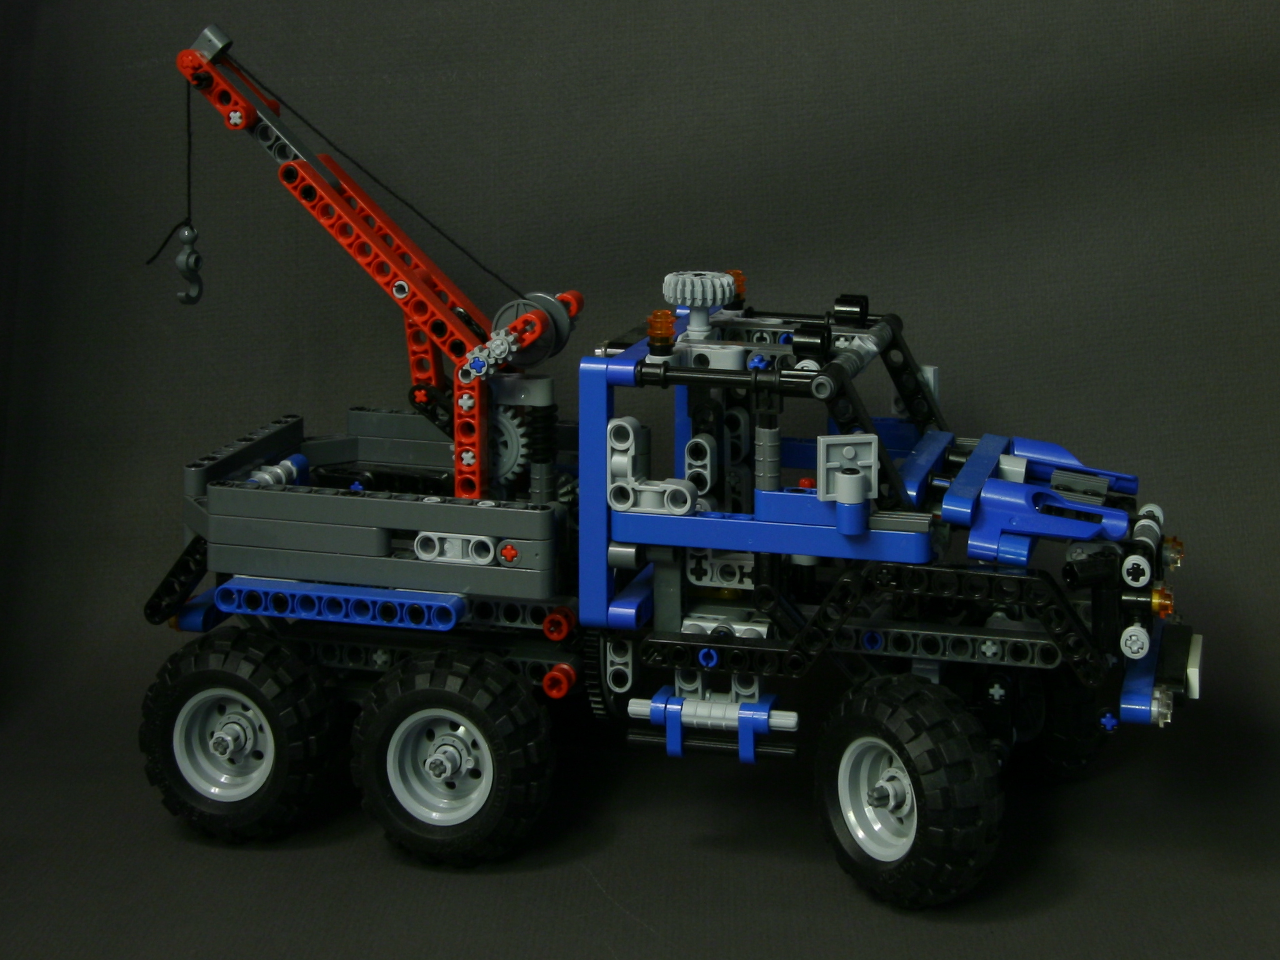
\includegraphics[width = 5cm, trim={15cm, 10cm, 15cm, 10cm}, clip]{images/layers_and_projections/legotruck/original/08_08}
			& & 
\includegraphics[width = 5cm, trim={7.5cm, 5cm, 7.5cm, 5cm}, clip]{figures/simulated_views/legotruck/3Layers_legotruck/Reconstruction_of_view_(3,3)}
		\end{tabular}
	\end{center}
\end{frame}

\begin{frame}[fragile]
	\frametitle{Example: Lego Truck}
	
	\begin{center}
		\begin{tabular}{c p{0cm} c}
			\begin{tabular}{@{}c@{}}Original \\ $17 \times 17 \times 960 \times 1280$\end{tabular}
			& & \begin{tabular}{@{}c@{}}Simulation (5 Layers) \\ $6 \times 6 \times 480 \times 640$\end{tabular} \\
			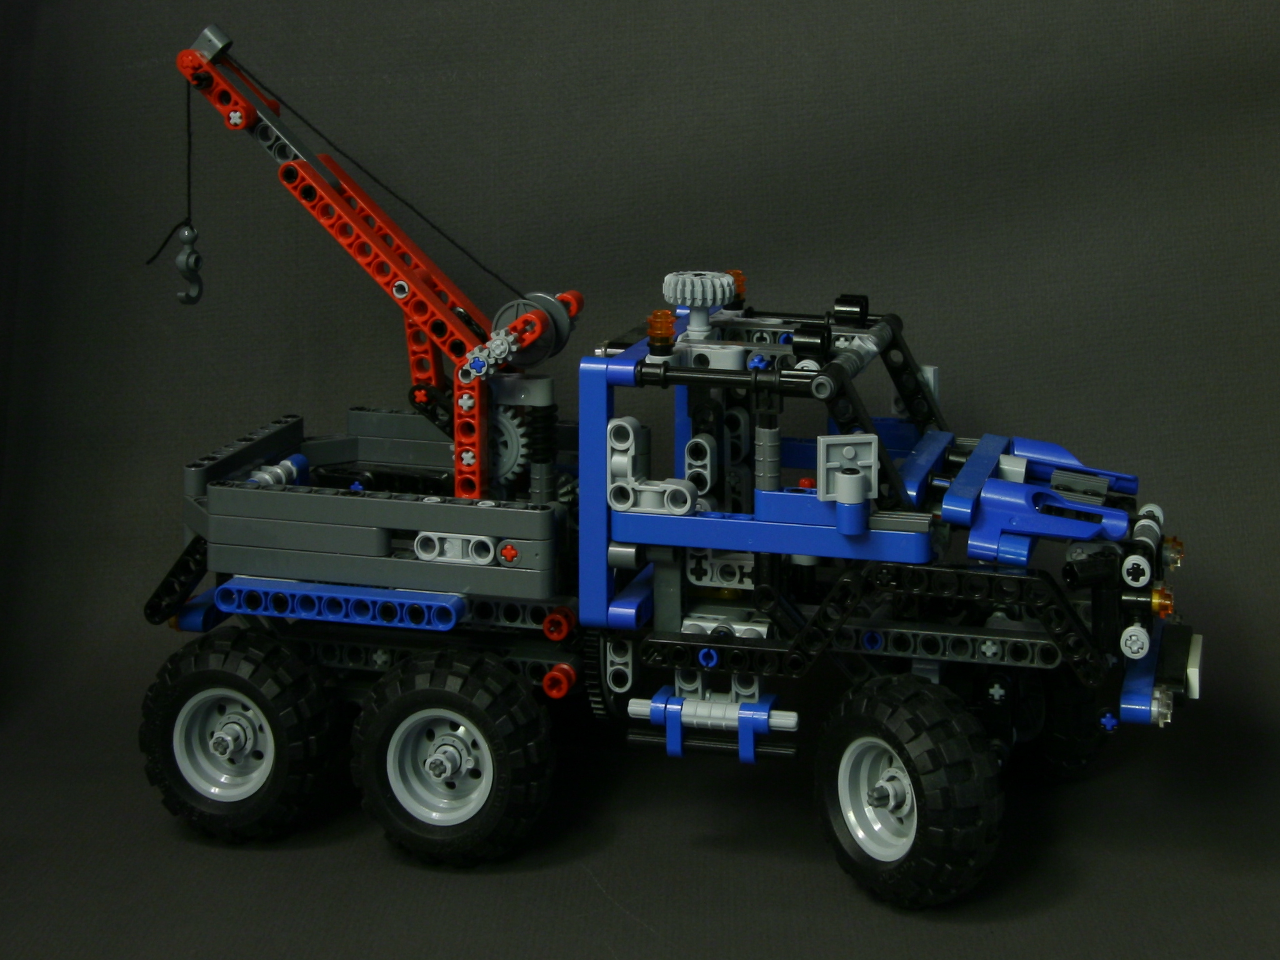
\includegraphics[width = 5cm, trim={15cm, 10cm, 15cm, 10cm}, clip]{images/layers_and_projections/legotruck/original/08_08}
			& & 
\includegraphics[width = 5cm, trim={7.5cm, 5cm, 7.5cm, 5cm}, clip]{figures/simulated_views/legotruck/5Layers_legotruck/Reconstruction_of_view_(3,3)}
		\end{tabular}
	\end{center}
\end{frame}

\begin{frame}[fragile]
	\frametitle{Example: Lego Truck}
	
	\begin{center}
		\begin{tabular}{c p{0cm} c}
			\begin{tabular}{@{}c@{}}Original \\ $17 \times 17 \times 960 \times 1280$\end{tabular}
			& & \begin{tabular}{@{}c@{}}Simulation (10 Layers) \\ $6 \times 6 \times 480 \times 640$\end{tabular} \\
			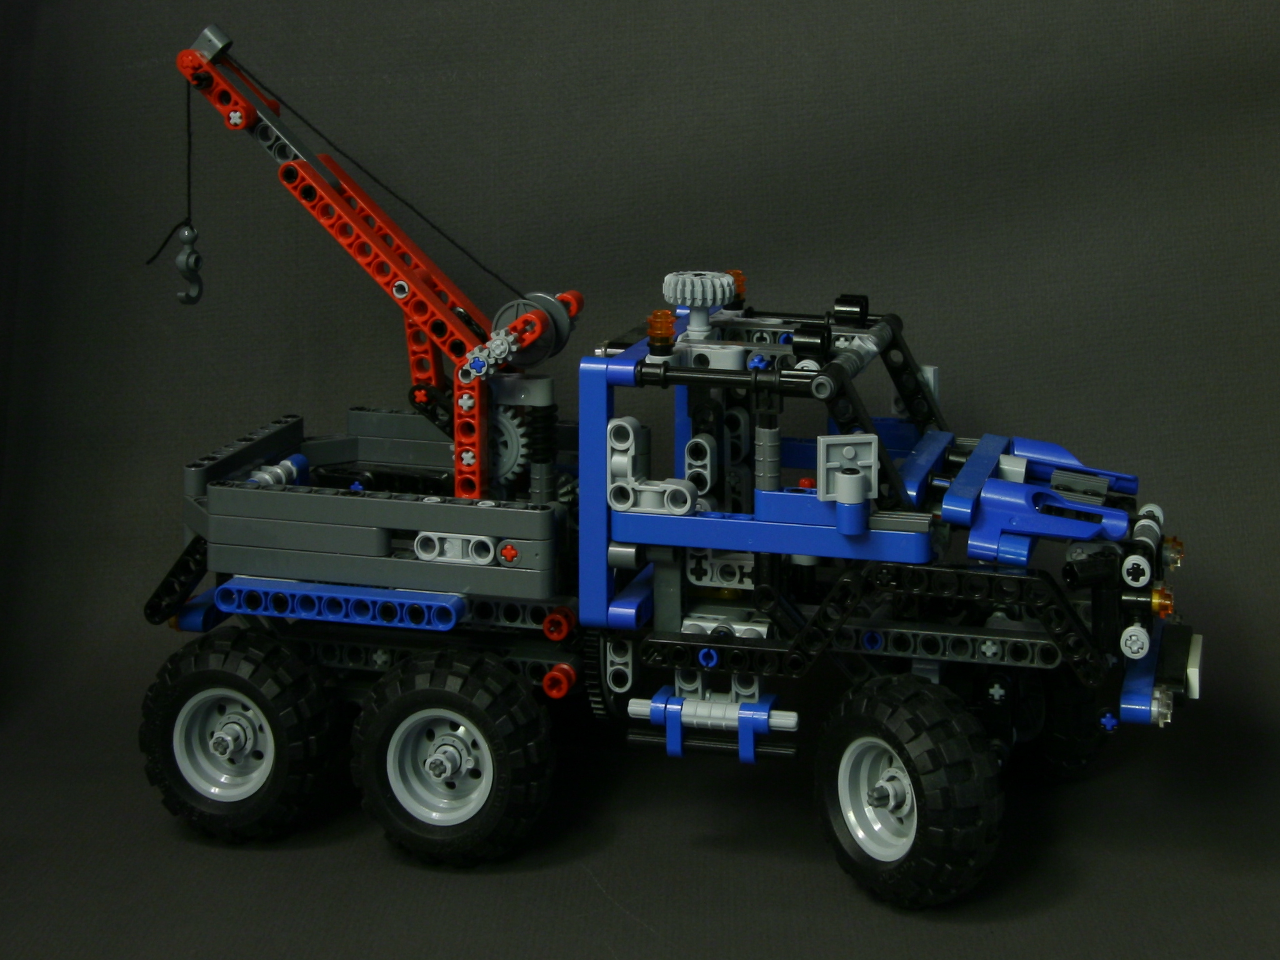
\includegraphics[width = 5cm, trim={15cm, 10cm, 15cm, 10cm}, clip]{images/layers_and_projections/legotruck/original/08_08}
			& & 
\includegraphics[width = 5cm, trim={7.5cm, 5cm, 7.5cm, 5cm}, clip]{figures/simulated_views/legotruck/10Layers_legotruck/Reconstruction_of_view_(3,3)}
		\end{tabular}
	\end{center}
\end{frame}

\begin{frame}[fragile]
	\frametitle{Example: Lego Truck}
%	\frametitle{10 Layers, Higher Angular Resolution}
	
	\begin{center}
		\begin{tabular}{c p{0cm} c}
			\begin{tabular}{@{}c@{}}Original \\ $17 \times 17 \times 960 \times 1280$\end{tabular}
			& & \begin{tabular}{@{}c@{}}Simulation (10 Layers) \\ $\textcolor{red}{9 \times 9} \times 480 \times 640$\end{tabular} \\
			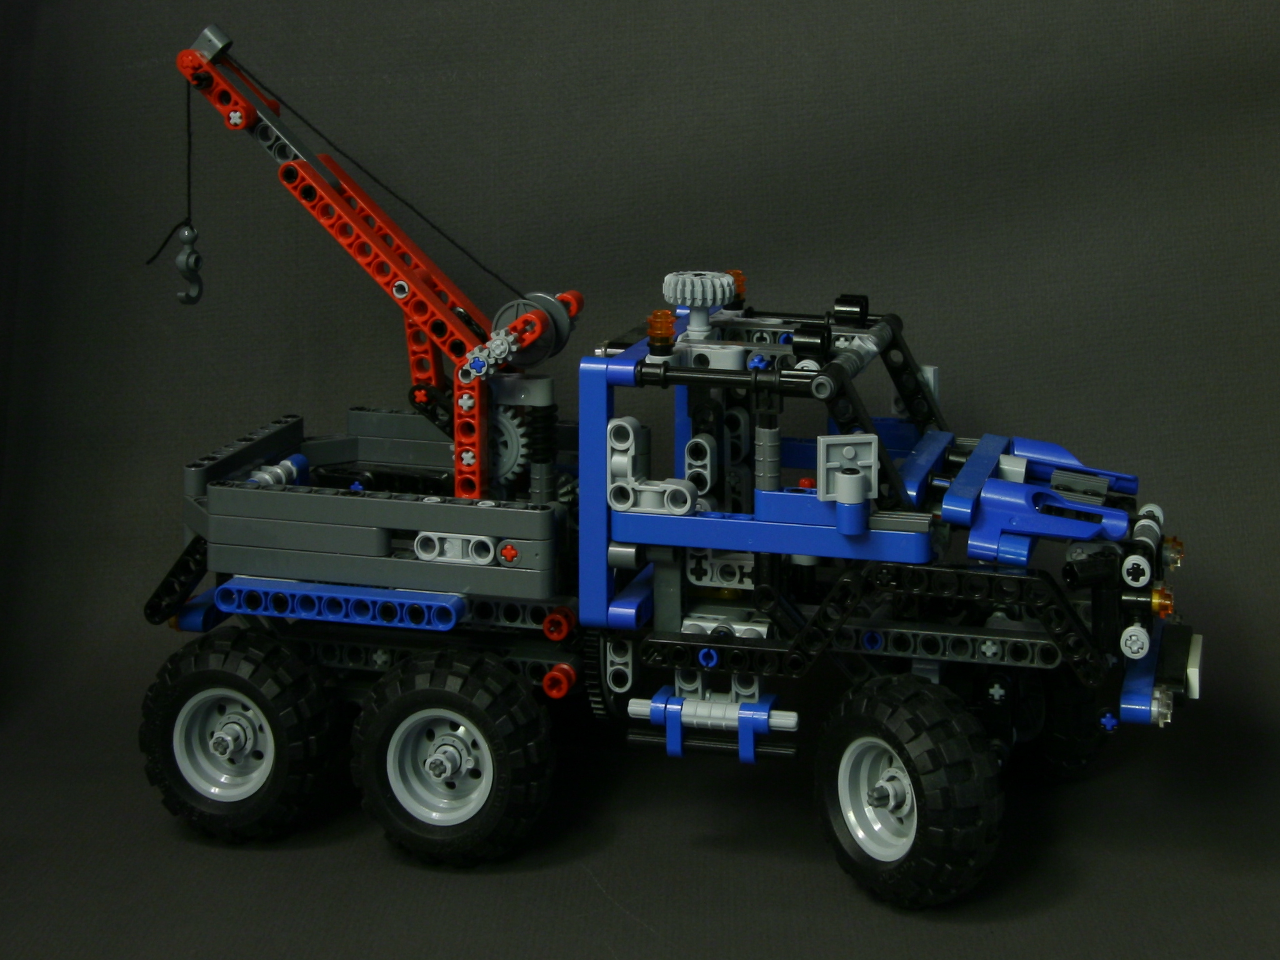
\includegraphics[width = 5cm, trim={15cm, 10cm, 15cm, 10cm}, clip]{images/layers_and_projections/legotruck/original/08_08}
			& & 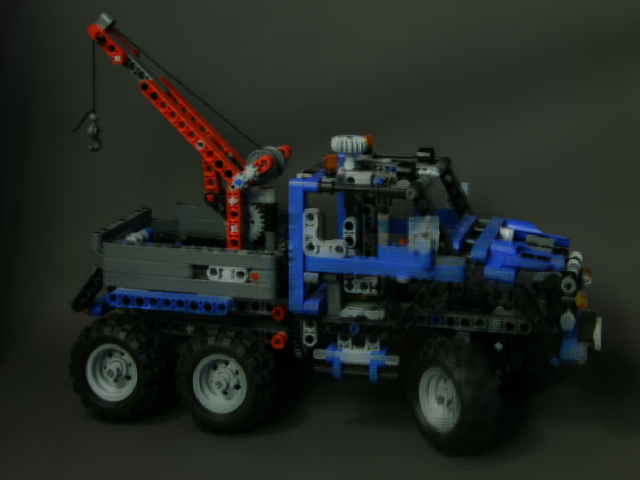
\includegraphics[width = 5cm, trim={7.5cm, 5cm, 7.5cm, 5cm}, clip]{figures/simulated_views/legotruck/10_Layers_9x9_angular/Reconstruction_of_view_(5,5)}
		\end{tabular}
	\end{center}
\end{frame}

\begin{frame}[fragile]
	\frametitle{Example: Lego Truck}
	
	\begin{columns}
		\column{0.3\textwidth}
			
\includegraphics[width = 3.1cm]{images/layers_and_projections/legotruck/3}
			\\
			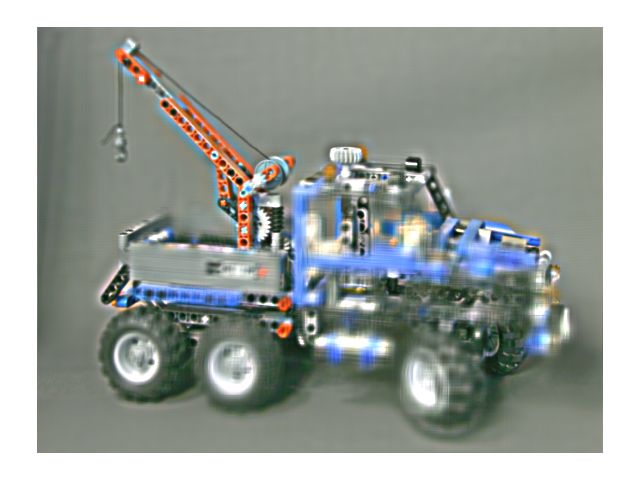
\includegraphics[width = 3.1cm]{images/layers_and_projections/legotruck/2}
			\\
			
\includegraphics[width = 3.1cm]{images/layers_and_projections/legotruck/1}
			\\
		\column{0.7\textwidth}
			\begin{itemize}
				\item \alert<1>{A lot of memory is needed:}
					\begin{itemize}
						\item Light field (uncompressed)
						\item Propagation matrix (? nnz entries)
						\item Additional matrices for solver
					\end{itemize}
				\item \alert<2>{Memory usage grows with resolution}
				\item \alert<3>{Solution: Slice the attenuator}
			\end{itemize}
	\end{columns}
	
\end{frame}

\begin{frame}[fragile]
	\frametitle{Attenuator Tiling}
	
	\begin{enumerate}[<alert@+>]
		\item Slice attenuator into smaller pieces
		\item Solve optimization problem for every slice
		\item Reconnect the slices
	\end{enumerate}
	
	\vspace{1cm}
	
	\begin{center}
		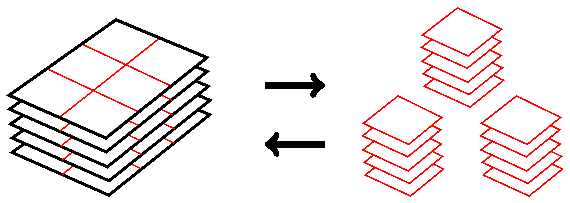
\includegraphics[height = 3cm]{figures/slicing_attenuator/tiling_overview.pdf}
	\end{center}
\end{frame}

\begin{frame}[fragile]
	\frametitle{Attenuator Tiling}

	\begin{itemize}
		\item Problem: Rays can overlap with multiple slices at borders
		\item Slices need to overlap too
		\item Blend slices with mask
	\end{itemize}
	
	\begin{figure}
		\subcaptionbox*{Original}{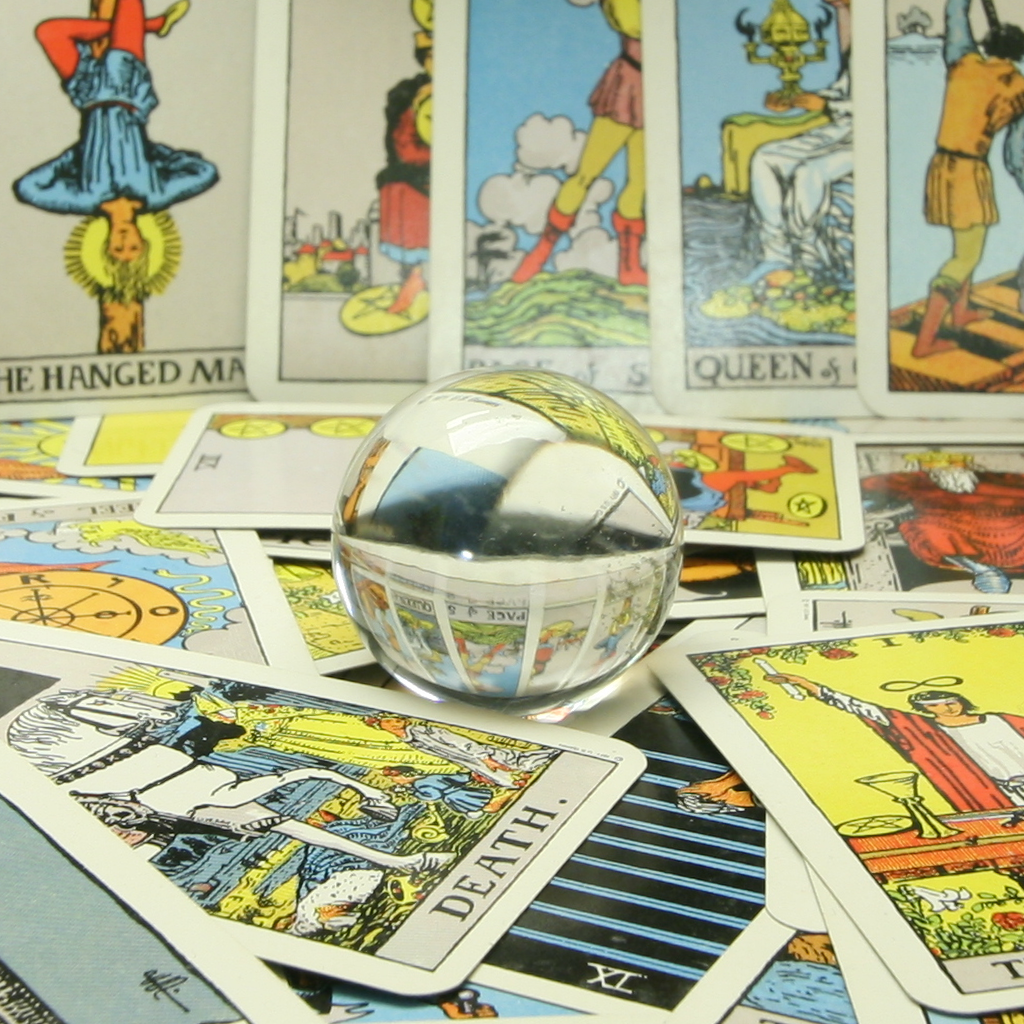
\includegraphics[width=4.3cm]{figures/tiling/original_08_08}}
		\hspace{1cm}
		\subcaptionbox*{Simulation}{
\includegraphics[width=4.3cm]{figures/tiling/tarot_tiles3x3x200x200_no_overlap_3_layers/Reconstruction_of_view_(3,3).png}}
	\end{figure}
	
	{\scriptsize Light field courtesy: \href{http://lightfield.stanford.edu/lfs.html}{Stanford Light Field Archive}}
\end{frame}

\begin{frame}[fragile]
	\frametitle{Tile Blending}

	\begin{figure}
		\documentclass{standalone}
\usepackage{tikz}

\begin{document}
	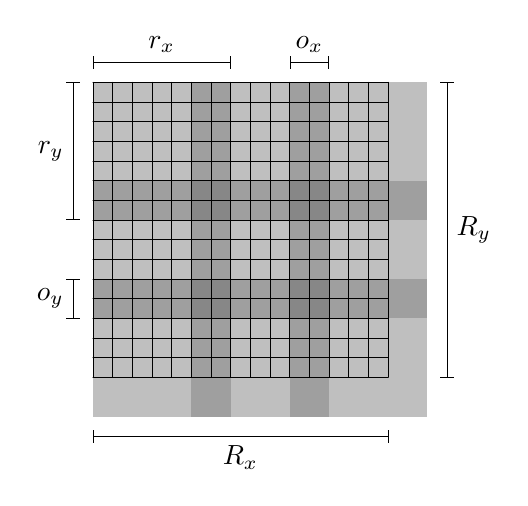
\begin{tikzpicture}[scale = 0.25, very thin]
	
		% Tiles
		\foreach \x in {0,...,2} {
			\foreach \y in {0,...,2}{
				\fill[gray, opacity = 0.5] (\x * 5, -\y * 5) rectangle ++(7, -7);
			}
		}
		
		% Grid
		\draw[step = 1 cm, cap = round] (0, 0) grid (15, -15);
		
		% Markers
		\draw[|-|] (0, -18) -- node[below]	{$R_x$} ++(15, 0);
		\draw[|-|] (18, 0) -- node[right]	{$R_y$} ++(0, -15);
		\draw[|-|] (0, 1) 	-- node[above]	{$r_x$} ++(7, 0);
		\draw[|-|] (-1, 0) 	-- node[left]	{$r_y$} ++(0, -7);
		\draw[|-|] (10, 1) 	-- node[above]	{$o_x$} ++(2, 0);
		\draw[|-|] (-1, -10) -- node[left]	{$o_y$} ++(0, -2);
	
	\end{tikzpicture}
\end{document}

		\documentclass{standalone}
\usepackage{calc}
\usepackage{tikz}

\begin{document}
	\begin{tikzpicture}[scale = 0.25, very thin]
	
		% Tiles
%		\foreach \x in {0,...,2} {
%			\foreach \y in {0,...,2}{
%				\fill[gray, opacity = 0.5] (\x * 5, -\y * 5) rectangle ++(7, -7);
%			}
%		}

		% Summed up masks
		\node<1>[anchor = north west, inner sep = 0] at (0, 0) {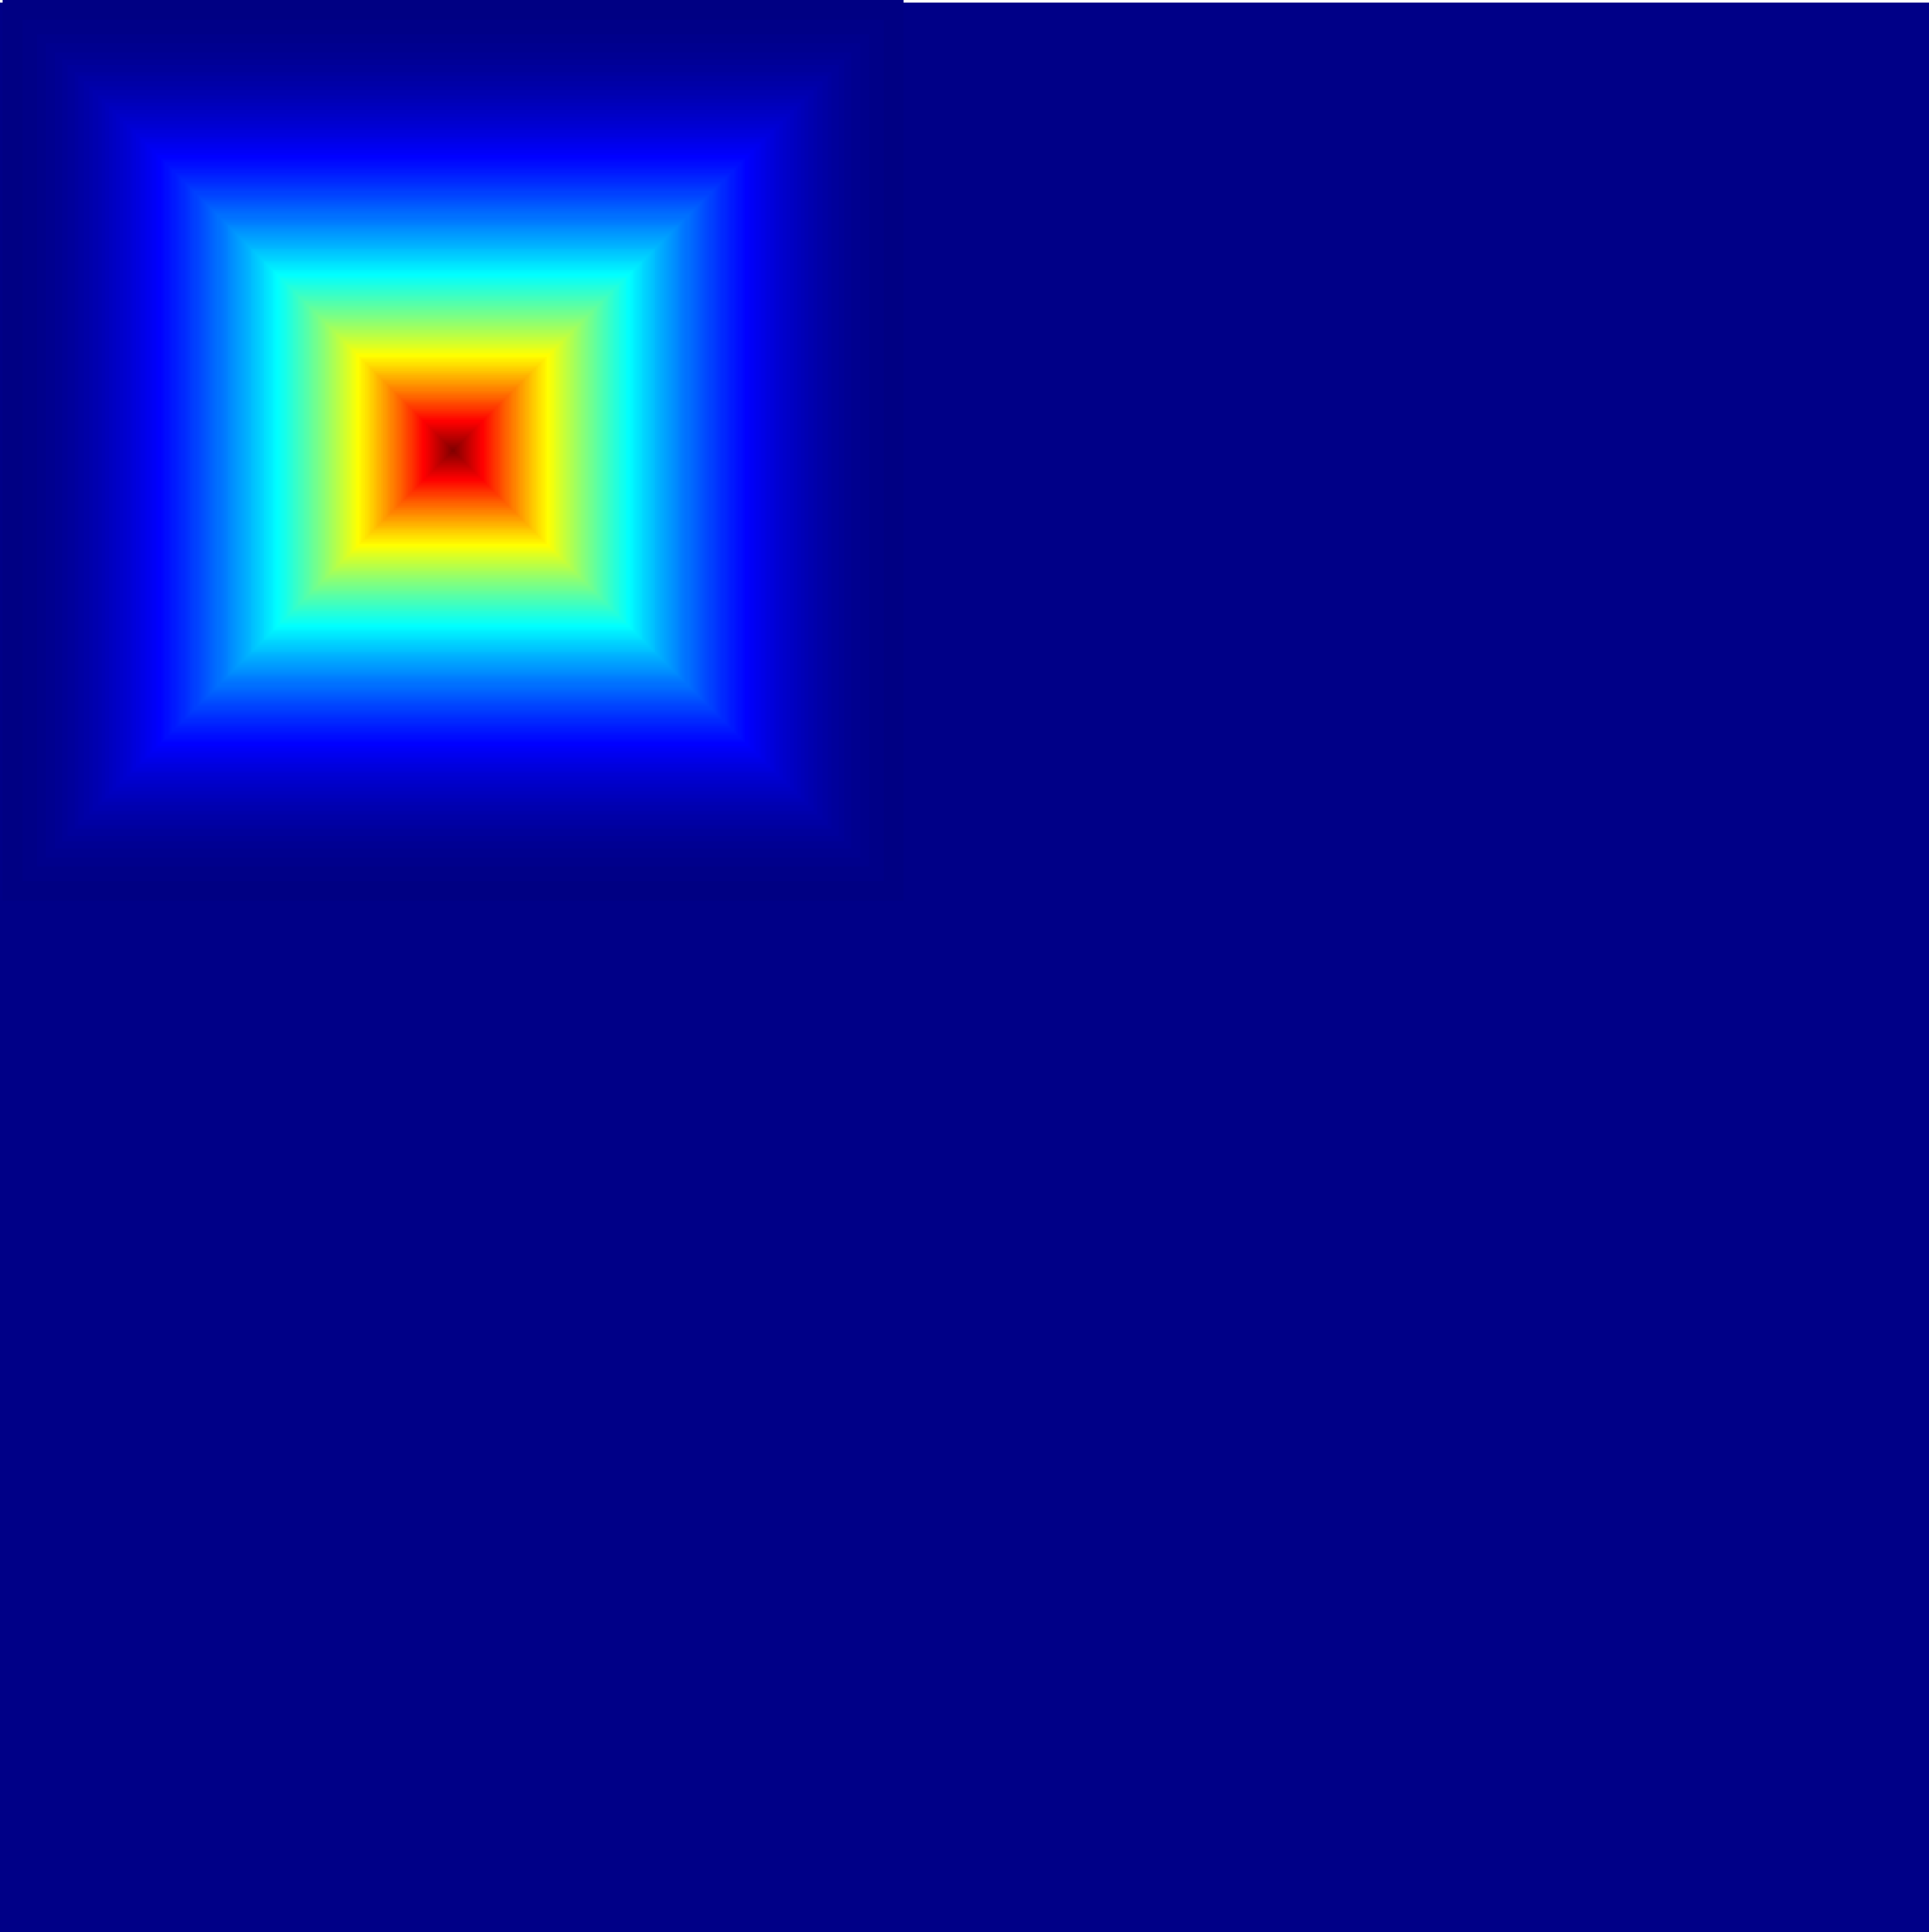
\includegraphics[width = 3.75cm]{./figures/tiling/mask1}};
		\node<2>[anchor = north west, inner sep = 0] at (0, 0) {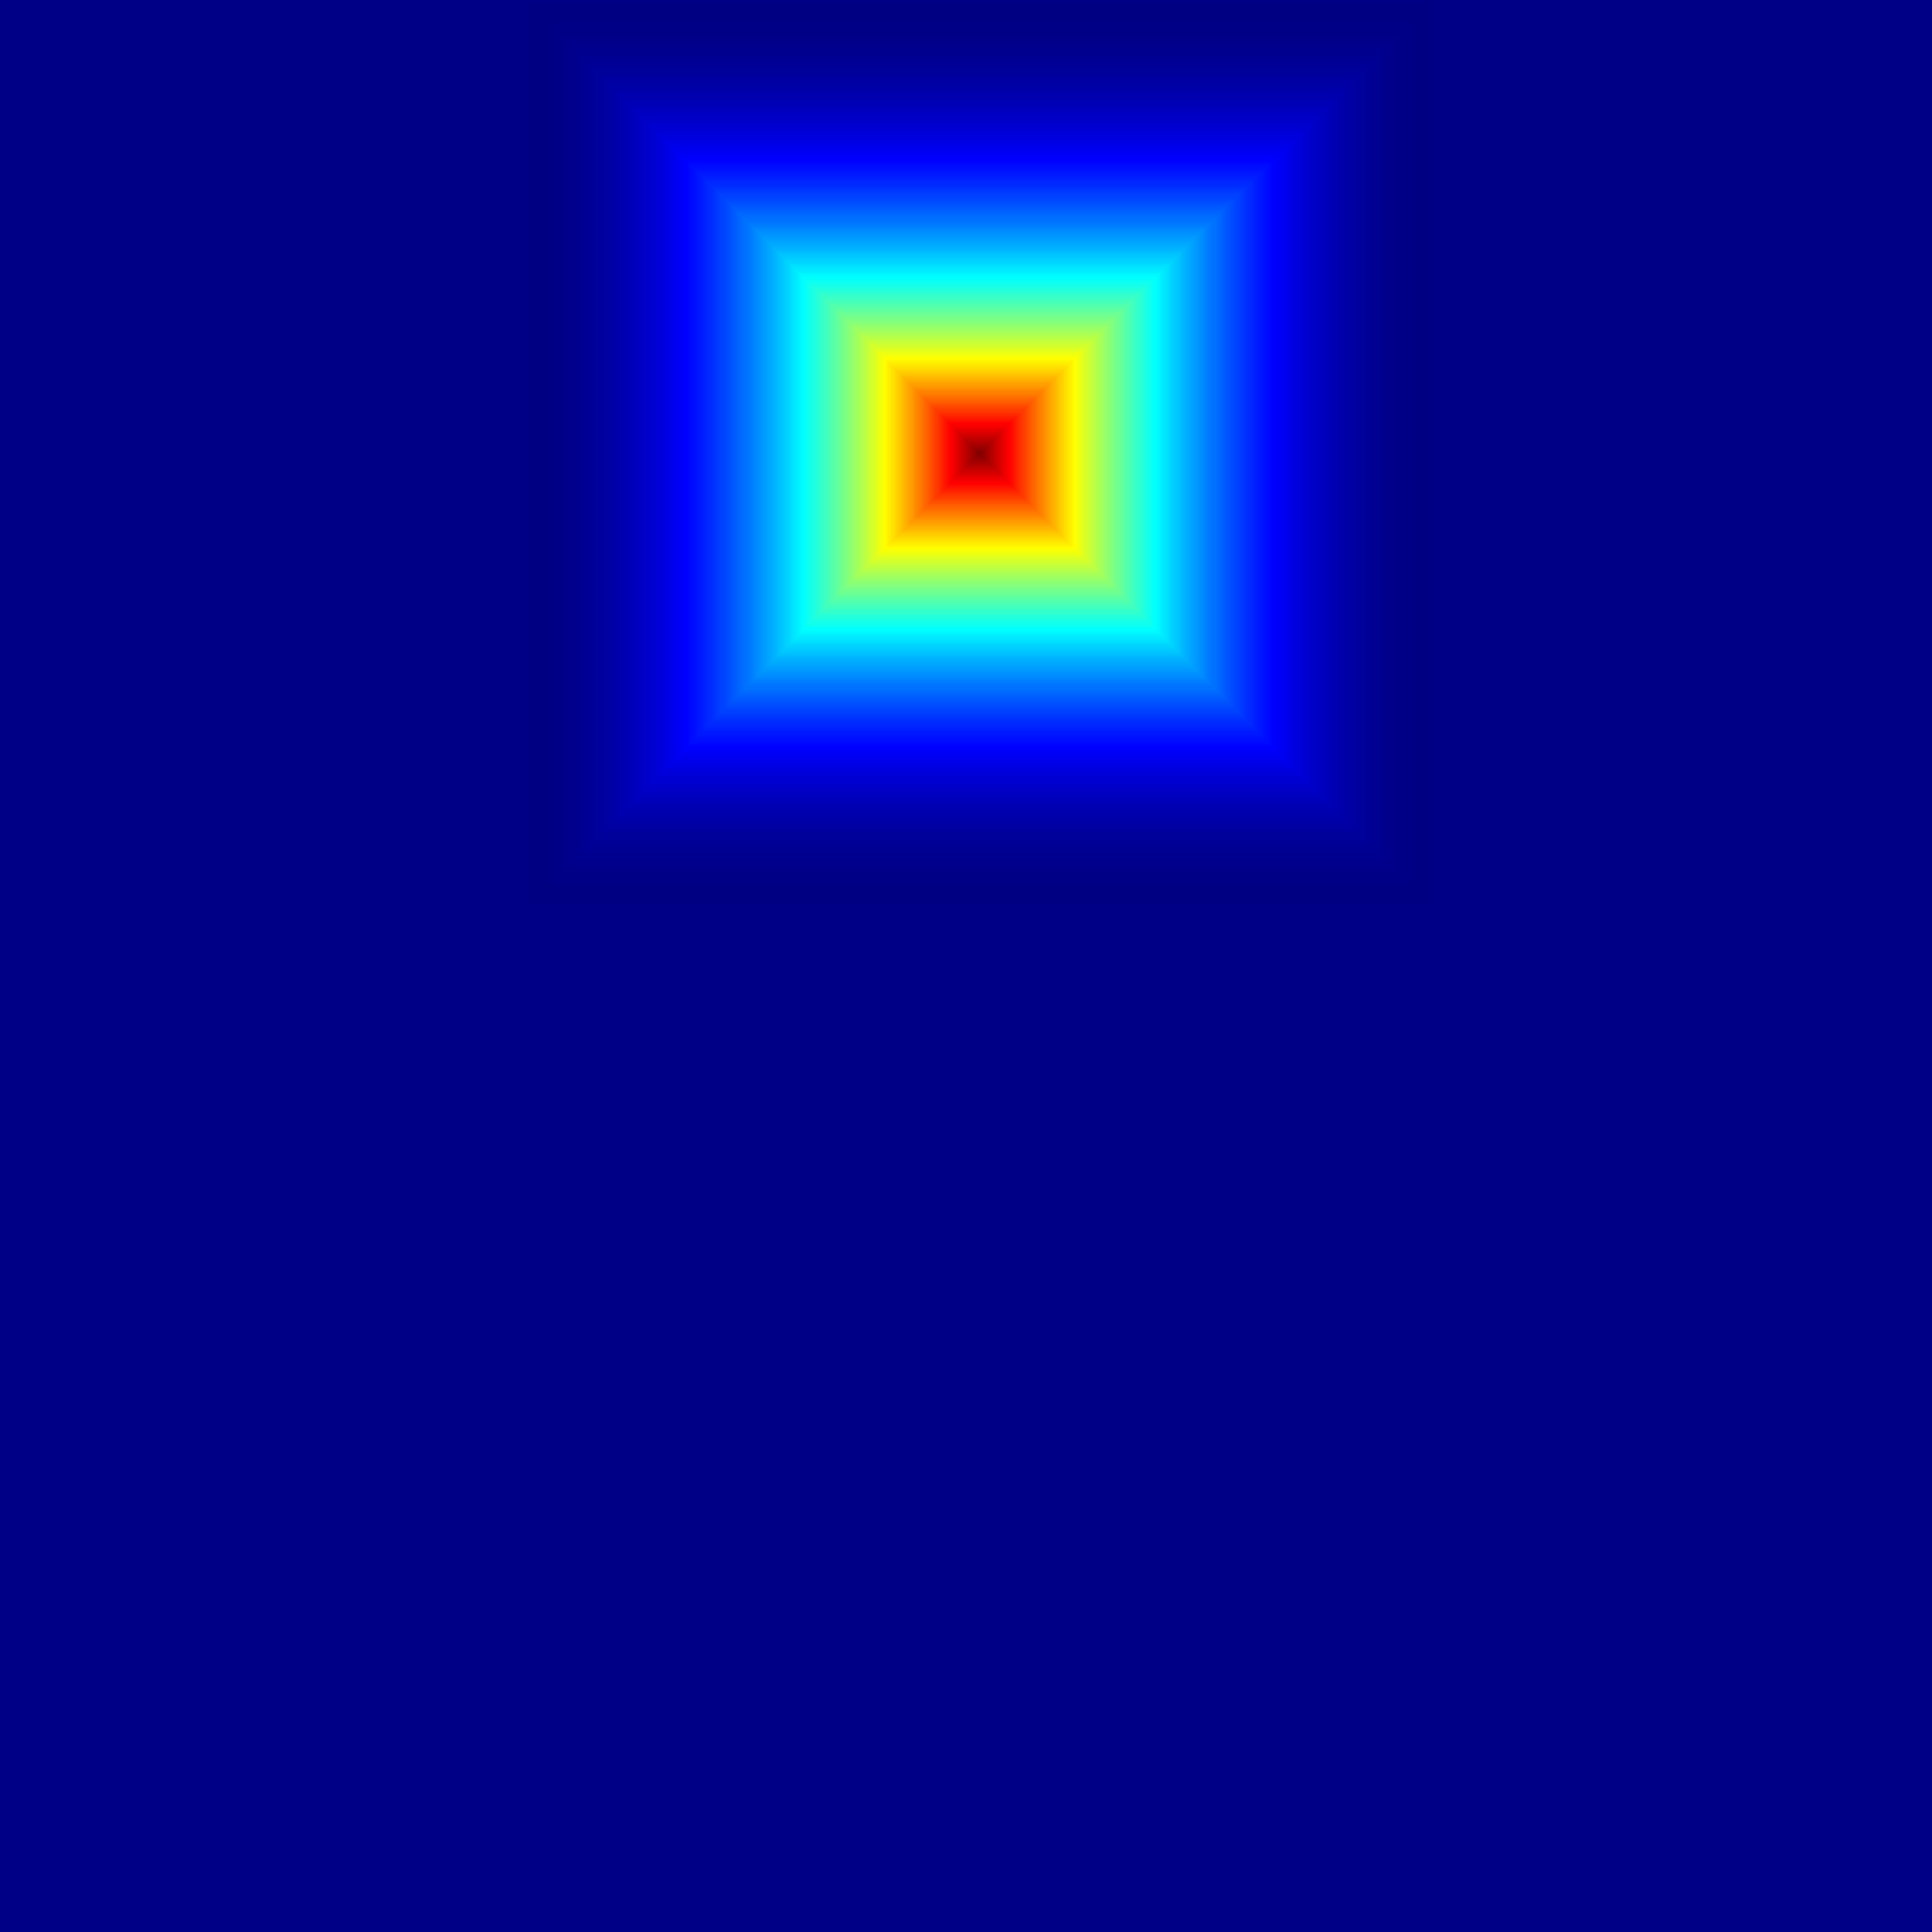
\includegraphics[width = 3.75cm]{./figures/tiling/mask2}};
		\node<3>[anchor = north west, inner sep = 0] at (0, 0) {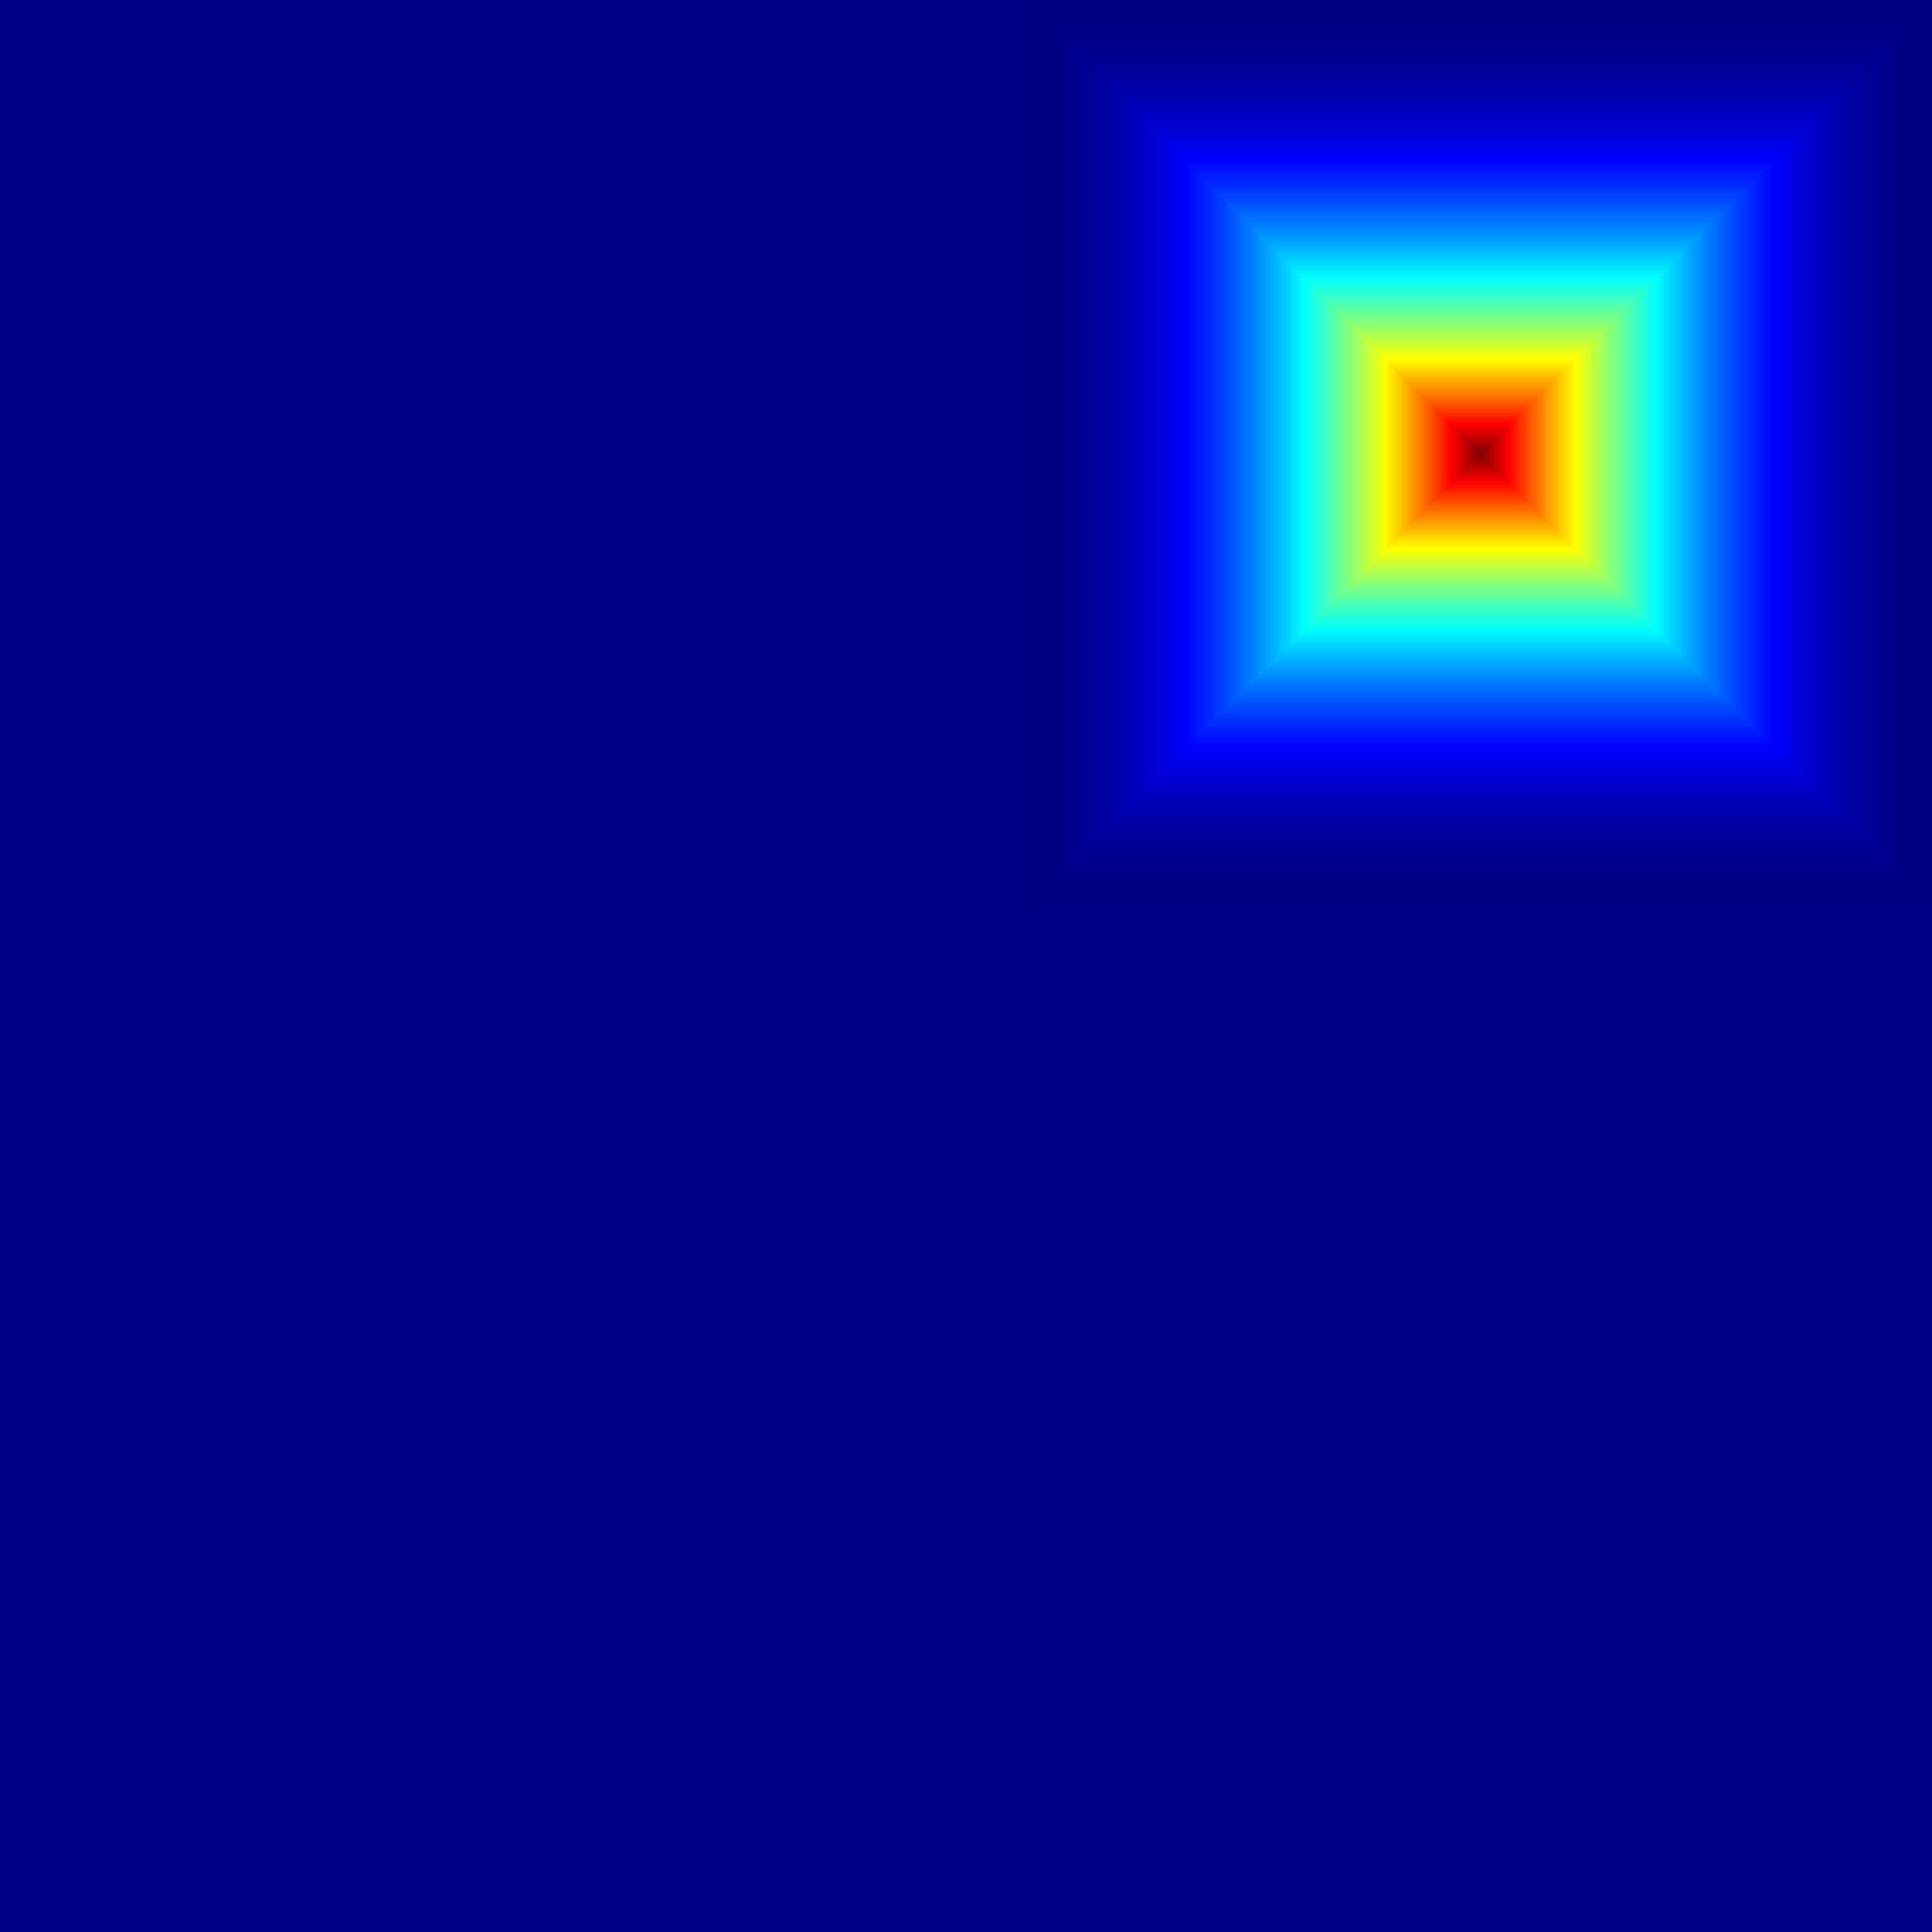
\includegraphics[width = 3.75cm]{./figures/tiling/mask3}};
		\node [anchor = east, scale=2] at (-0.5, -7.5) {$\ast$};
		% Grid
%		\draw[step = 1 cm, cap = round] (0, 0) grid (15, -15);
		
		% Invisible markers for accurate placement in figure 
		\begin{scope}[opacity = 0]
			\draw[|-|] (0, -18) -- node[below]	{$R_x$} ++(15, 0);
%			\draw[|-|] (18, 0) -- node[right]	{$R_y$} ++(0, -15);
			\draw[|-|] (0, 1) 	-- node[above]	{$r_x$} ++(7, 0);
%			\draw[|-|] (-1, 0) 	-- node[left]	{$r_y$} ++(0, -7);
			\draw[|-|] (10, 1) 	-- node[above]	{$o_x$} ++(2, 0);
%			\draw[|-|] (-1, -10) -- node[left]	{$o_y$} ++(0, -2);
		\end{scope}
		
	\end{tikzpicture}
\end{document}
	\end{figure}
\end{frame}

\begin{frame}[fragile]
	\frametitle{Tile Blending}
	
	\begin{figure}
		\subcaptionbox*{No overlap}{
\includegraphics[width=5cm]{figures/tiling/tarot_tiles3x3x200x200_no_overlap_3_layers/Reconstruction_of_view_(3,3).png}}
		\hspace{0.5cm}
		\subcaptionbox*{30\% overlap}{
\includegraphics[width=5cm]{figures/tiling/tarot_tiles5x5x200x200_overlap0.5_3_layers/Reconstruction_of_view_(3,3).png}}
	\end{figure}
\end{frame}

\begin{frame}[fragile]
	\frametitle{The Finished Display}
	
	\begin{itemize}
		\item Finally, print images on transparent sheets
		\item Glass plates hold sheets in place
		\item Combine with backlight
	\end{itemize}
	
	\begin{center}
		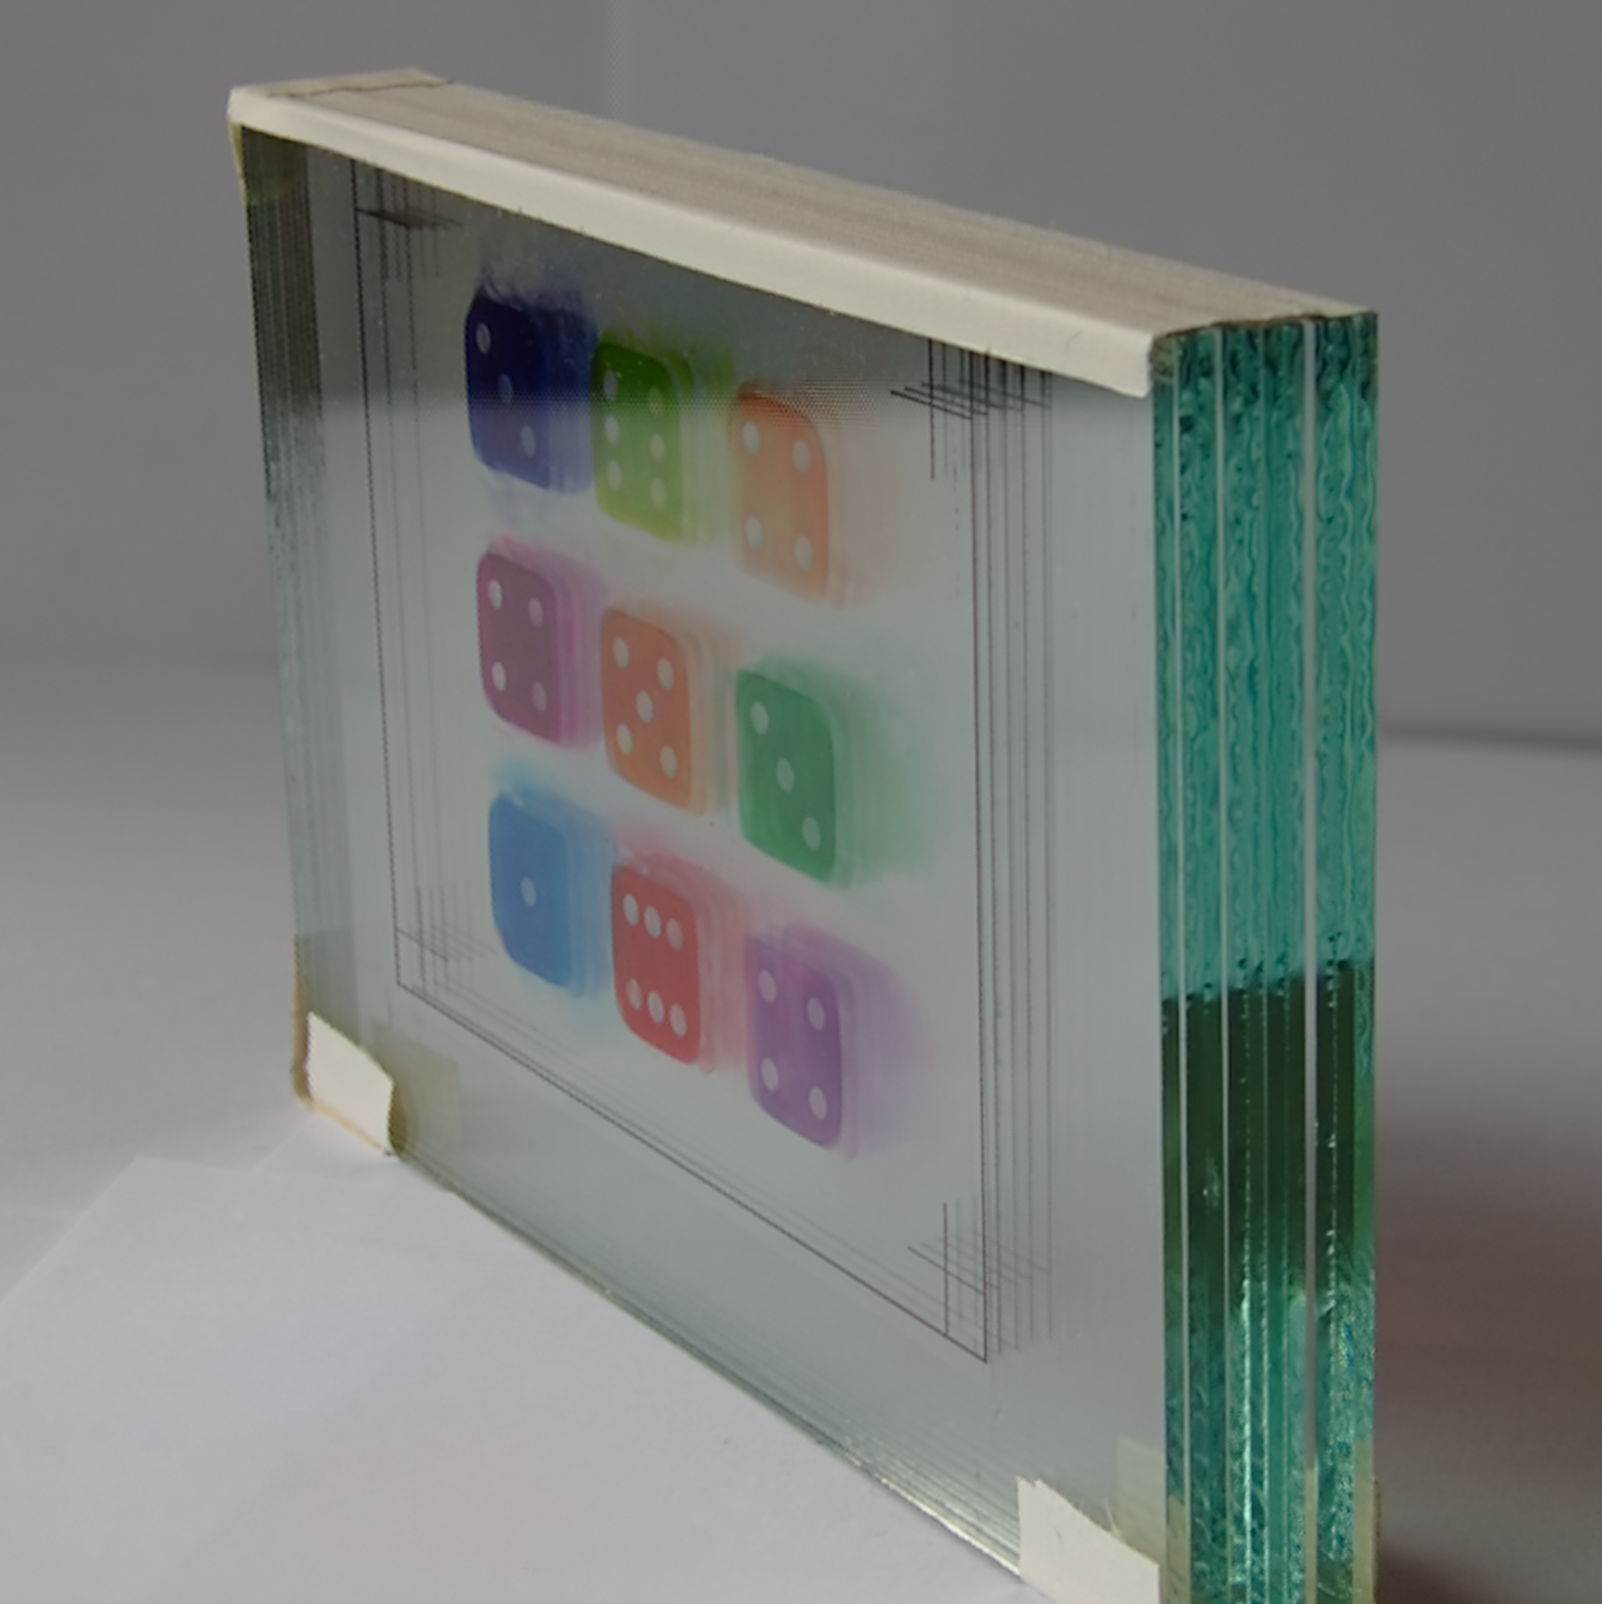
\includegraphics[height=4cm]{images/glass_plates_front_view_cropped}
		\hspace{1cm}
		\includegraphics[height=4cm]{images/raw_backlight_from_top}
	\end{center}
\end{frame}

\begin{frame}[fragile]
	\frametitle{The Finished Product}
	\begin{center}
		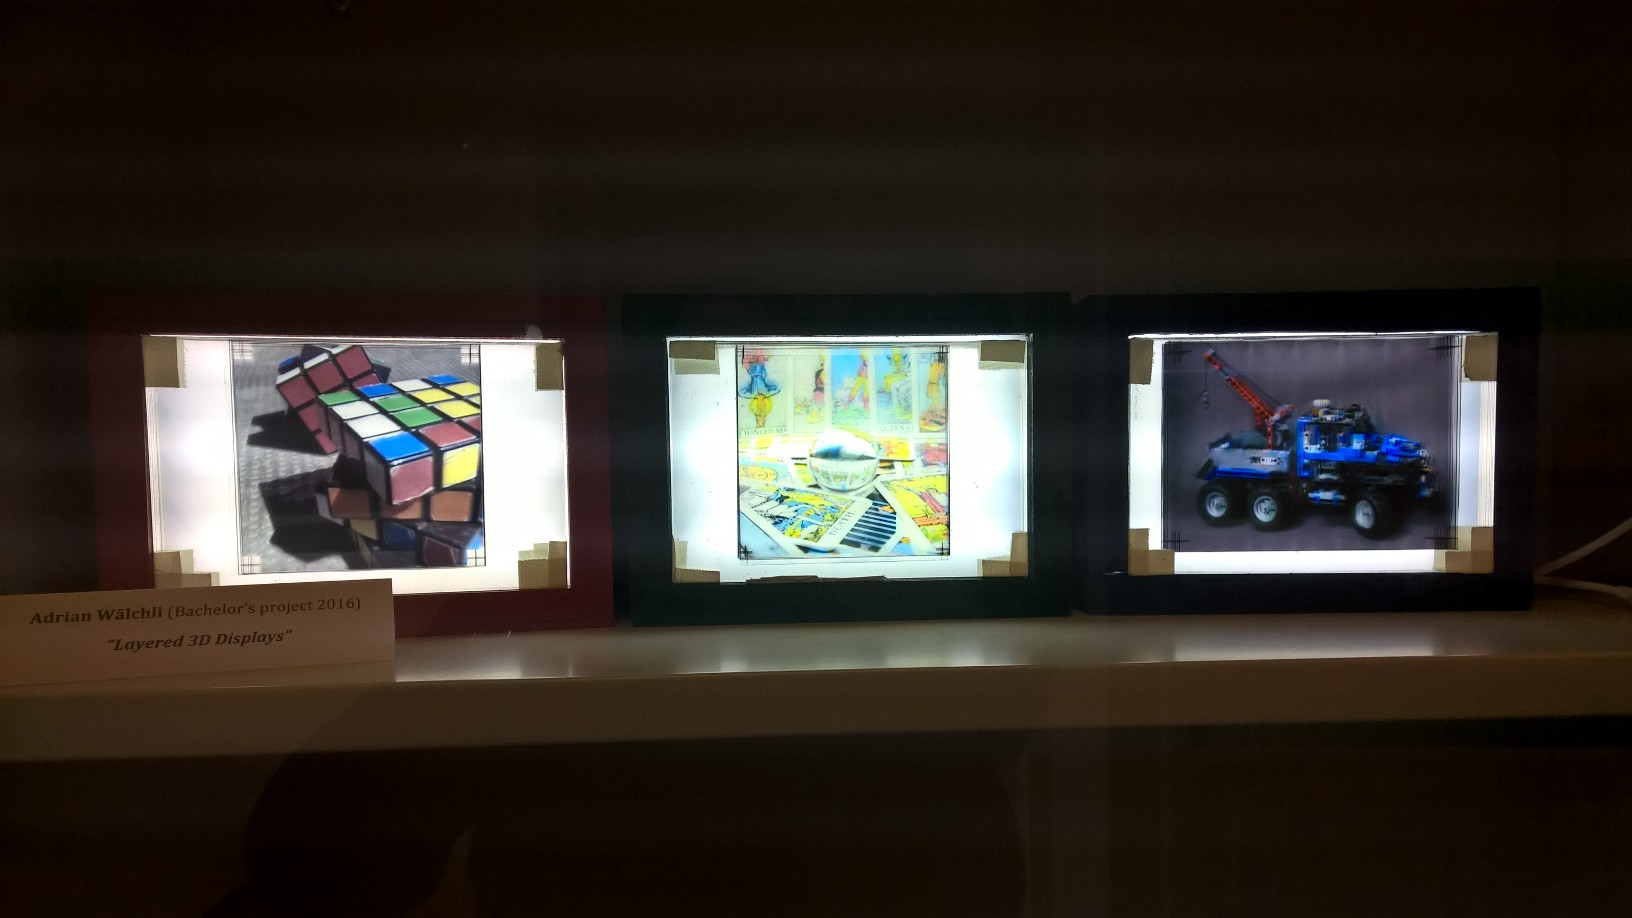
\includegraphics[width=11cm]{images/all_displays_on}
	\end{center}
\end{frame}

\begin{frame}[fragile]
	\frametitle{Questions}
	
	\begin{itemize}[<+- | alert@+>]
		\item Impact of more layers?
		\item Does thickness of display matter?
		\item Is it possible to show objects outside the display?
		\item What are the limitations?
	\end{itemize}
\end{frame}

\section{Spectral Analysis}

%\begin{frame}[fragile]
%	\frametitle{Epipolar Plane Geometry}
%	\begin{figure}
%		\captionsetup{font=scriptsize}
%		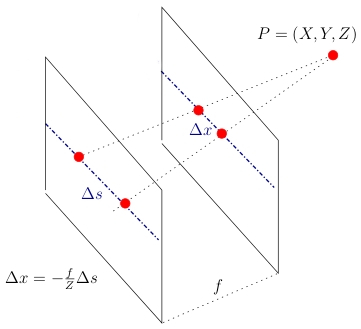
\includegraphics[height = 6cm]{images/lf_geometry_modified.jpg}
%		\caption*{Source: \href{http://klimt.iwr.uni-heidelberg.de/HCI/Research/LightField/images/lf_geometry.jpg}{klimt.iwr.uni-heidelberg.de}}
%	\end{figure}
%\end{frame}

\begin{frame}[fragile]
	\frametitle{Epipolar Plane Image}
	
	\begin{center}
		\documentclass{standalone}
\usepackage{tikz}
\usepackage{pgfplots}

\tikzset{align at bottom/.style={baseline=(current bounding box.south)}}

\begin{document} 
	\begin{tikzpicture}[scale = 0.27]
	
		\draw[->] (-5, 0) -- (5, 0) node[right] {$s$};
		\draw[<-] (-5, -5) -- (-5, 5) node[above] {$z$};
	
		\begin{scope}
			\clip (-5, -5) rectangle (5, 5);
			\draw[scale = 1, smooth, domain = -10 : 10, variable = \x, black, dashed] plot ({\x}, {3});
			\draw[scale = 1, smooth, domain = -10 : 10, variable = \x, black, dashed] plot ({\x}, {-2});
		\end{scope}
		
		\node[left] at (-5, 3) {$Z_\textrm{min}$};
		\node[left] at (-5, -2) {$Z_\textrm{max}$};
		
		\draw[ultra thick, blue] (0, 3) -- (2, 3);
		\draw[ultra thick, red] (-3, -2) -- (0, -2);
		
		% Phantom node for alignment
		\node[right, opacity = 0] at (-5, -5) {$s$};
		
	\end{tikzpicture}
\end{document}
		\hspace{1cm}
		\documentclass{standalone}
\usepackage{tikz}
\usepackage{pgfplots}

\tikzset{align at bottom/.style={baseline=(current bounding box.south)}}

\begin{document} 
	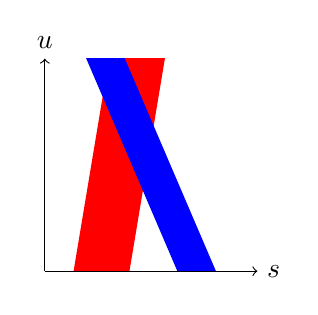
\begin{tikzpicture}[scale = 0.27]
	
		\begin{scope}
			\clip (-5, -5) rectangle (5, 5);
			\draw[scale = 1, smooth, variable = \x, red, line width = 0.7cm] plot ({\x}, { 12 / 2 * (\x + 1.5)});
			\draw[scale = 1, smooth, variable = \x, blue, line width = 0.45cm] plot ({\x}, { -7 / 3 * \x});
		\end{scope}
		
		\draw[->] (-5, -5) -- (5, -5) node[right] {$s$};
		\draw[->] (-5, -5) -- (-5, 5) node[above] {$u$};
		
	\end{tikzpicture}
\end{document}
	\end{center}
	
	\begin{equation*}
		\frac{\text{d}u}{\text{d}s} = \frac{z - Z_u}{z - Z_s}
	\end{equation*}
	
\end{frame}

\begin{frame}[fragile]
	\frametitle{Spectral Properties of Light Fields}
	
	\begin{figure}
		\documentclass{standalone}
\usepackage{tikz}
\usepackage{pgfplots}

\tikzset{align at bottom/.style={baseline=(current bounding box.south)}}

\begin{document} 
	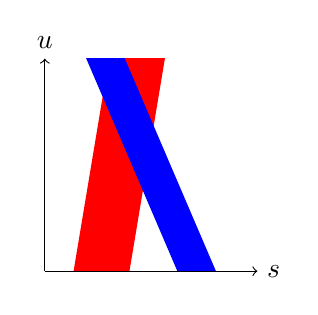
\begin{tikzpicture}[scale = 0.27]
	
		\begin{scope}
			\clip (-5, -5) rectangle (5, 5);
			\draw[scale = 1, smooth, variable = \x, red, line width = 0.7cm] plot ({\x}, { 12 / 2 * (\x + 1.5)});
			\draw[scale = 1, smooth, variable = \x, blue, line width = 0.45cm] plot ({\x}, { -7 / 3 * \x});
		\end{scope}
		
		\draw[->] (-5, -5) -- (5, -5) node[right] {$s$};
		\draw[->] (-5, -5) -- (-5, 5) node[above] {$u$};
		
	\end{tikzpicture}
\end{document}
		\hspace{1cm}
		\only<1>{
			\subcaptionbox*{\centering Frequency Response (Amplitude)}{\documentclass{standalone}
\usepackage{tikz}
\usepackage{pgfplots}

\tikzset{align at bottom/.style={baseline=(current bounding box.south)}}

\begin{document}
	\begin{tikzpicture}[scale = 0.35]
	
		\begin{scope}
			\clip (-5, -5) rectangle (5, 5);
			%\node[anchor = center, inner sep = 0, opacity = 0.4] at (0, 0) {\includegraphics[width = 5cm]{../Figures/spectral_support/fft_red_and_blue.png}};
		\end{scope}
		
		\draw[->] (-5, 0) -- (5, 0) node[right] {$\xi_s$};
		\draw[->] (0, -5) -- (0, 5) node[above] {$\xi_u$};
		
		% Invisible dummy node for symmetric alignment with caption
		\node[left, opacity = 0] at (-5, 0) {$\xi_s$};
		
		\begin{scope}
			\clip (-5, -5) rectangle (5, 5);
			\draw[scale=1, smooth, domain = -10 : 10, variable = \x, blue] plot ({\x},{ -1 / (- 7 / 3) * \x});
			\draw[scale=1, smooth, domain = -10 : 10, variable = \x, red] plot ({\x},{ -1 / (12 / 2) * \x});
		\end{scope}
		
	\end{tikzpicture}
\end{document}}	
		}
		\only<2>{
			\subcaptionbox*{\centering Frequency Response (Amplitude)}{\documentclass{standalone}
\usepackage{tikz}
\usepackage{pgfplots}

\tikzset{align at bottom/.style={baseline=(current bounding box.south)}}

\begin{document}
	\begin{tikzpicture}[scale = 0.27]
	
		\begin{scope}
			\clip (-5, -5) rectangle (5, 5);
%			\clip (-4.5, -4.5) rectangle (4.5, 4.5);
			\node[anchor = center, inner sep = 0, opacity = 1] at (0, 0) {\includegraphics[width = 5cm]{figures/spectral_support/fft_red_and_blue.png}};
		\end{scope}
		
		\begin{scope}
			\draw[->, opacity = 1] (-5, 0) -- (5, 0) node[right, opacity = 1] {$\xi_s$};
			\draw[->, opacity = 1] (0, -5) -- (0, 5) node[above, opacity = 1] {$\xi_u$};
		\end{scope}
		
		% Invisible dummy node for symmetric alignment with caption
		\node[left, opacity = 0] at (-5, 0) {$\xi_s$};
		
	\end{tikzpicture}
\end{document}}	
		}
	\end{figure}
\end{frame}

\begin{frame}[fragile]
	\frametitle{Spectral Properties of Display}
	
	\begin{itemize}[<alert@+>]
		\item Every layer creates a light field $L_n$
		\item Stack of layers creates $L^\prime = L_0 \cdot L_1 \cdots L_N$
		\item What does $L^\prime$ look like in frequency domain?
	\end{itemize}
	
	\begin{figure}
		\subcaptionbox*{Layer 1}{\documentclass{standalone}
\usepackage{tikz}
\usetikzlibrary{intersections}

\tikzset{align at bottom/.style={baseline=(current bounding box.south)}}

\begin{document}
	\begin{tikzpicture}[scale = 0.27]
	
		\draw[->] (-5, 0) -- (5, 0) node[right] {$\xi_s$};
		\draw[->] (0, -5) -- (0, 5) node[above] {$\xi_u$};
		
		% Invisible dummy node for symmetric alignment with caption
%		\node[left, opacity = 0] at (-5, 0) {$\xi_s$};
		
		%\draw[draw = black, fill = gray, fill opacity = 0.2, draw opacity = 0.5, name path = support_cut_off] (-4, 0) -- (-1.5, 3) -- (1.5, 3) -- (4, 0) -- (1.5, -3) -- (-1.5, -3) -- cycle;
		
		\begin{scope}
		
			\clip (-2, -2) rectangle (2, 2);
			
			\draw[red, thick, cap = round] (-2, 1) -- (2, -1);
%			\draw[red, thick, cap = round] (-2, 0) -- (2, 0);
%			\draw[red, thick, cap = round] (-2, -1) -- (2, 1);
			
		\end{scope}
		
		\draw[black, cap = round, dotted] (-2, 2.5) -- (-2, -2.5);
		\draw[black, cap = round, dotted] (2, 2.5) -- (2, -2.5);
		
%		\node[below] at (-2, -2.5) {$-\xi_0$};
%		\node[below] at (2, -2.5) {$\xi_0$};
		
	\end{tikzpicture}
	
\end{document}}
		\subcaptionbox*{Layer 2}{\documentclass{standalone}
\usepackage{tikz}
\usetikzlibrary{intersections}

\tikzset{align at bottom/.style={baseline=(current bounding box.south)}}

\begin{document}
	\begin{tikzpicture}[scale = 0.27]
	
		\draw[->] (-5, 0) -- (5, 0) node[right] {$\xi_s$};
		\draw[->] (0, -5) -- (0, 5) node[above] {$\xi_u$};
		
		% Invisible dummy node for symmetric alignment with caption
%		\node[left, opacity = 0] at (-5, 0) {$\xi_s$};
		
		%\draw[draw = black, fill = gray, fill opacity = 0.2, draw opacity = 0.5, name path = support_cut_off] (-4, 0) -- (-1.5, 3) -- (1.5, 3) -- (4, 0) -- (1.5, -3) -- (-1.5, -3) -- cycle;
		
		\begin{scope}
		
			\clip (-2, -2) rectangle (2, 2);
			
%			\draw[red, thick, cap = round] (-2, 1) -- (2, -1);
			\draw[red, thick, cap = round] (-2, 0) -- (2, 0);
%			\draw[red, thick, cap = round] (-2, -1) -- (2, 1);
			
		\end{scope}
		
		\draw[black, cap = round, dotted] (-2, 2.5) -- (-2, -2.5);
		\draw[black, cap = round, dotted] (2, 2.5) -- (2, -2.5);
		
%		\node[below] at (-2, -2.5) {$-\xi_0$};
%		\node[below] at (2, -2.5) {$\xi_0$};
		
	\end{tikzpicture}
	
\end{document}}
		\subcaptionbox*{Layer 3}{\documentclass{standalone}
\usepackage{tikz}
\usetikzlibrary{intersections}

\tikzset{align at bottom/.style={baseline=(current bounding box.south)}}

\begin{document}
	\begin{tikzpicture}[scale = 0.27]
	
		\draw[->] (-5, 0) -- (5, 0) node[right] {$\xi_s$};
		\draw[->] (0, -5) -- (0, 5) node[above] {$\xi_u$};
		
		% Invisible dummy node for symmetric alignment with caption
%		\node[left, opacity = 0] at (-5, 0) {$\xi_s$};
		
		%\draw[draw = black, fill = gray, fill opacity = 0.2, draw opacity = 0.5, name path = support_cut_off] (-4, 0) -- (-1.5, 3) -- (1.5, 3) -- (4, 0) -- (1.5, -3) -- (-1.5, -3) -- cycle;
		
		\begin{scope}
		
			\clip (-2, -2) rectangle (2, 2);
			
%			\draw[red, thick, cap = round] (-2, 1) -- (2, -1);
%			\draw[red, thick, cap = round] (-2, 0) -- (2, 0);
			\draw[red, thick, cap = round] (-2, -1) -- (2, 1);
			
		\end{scope}
		
		\draw[black, cap = round, dotted] (-2, 2.5) -- (-2, -2.5);
		\draw[black, cap = round, dotted] (2, 2.5) -- (2, -2.5);
		
%		\node[below] at (-2, -2.5) {$-\xi_0$};
%		\node[below] at (2, -2.5) {$\xi_0$};
		
	\end{tikzpicture}
	
\end{document}}
	\end{figure}
\end{frame}

\begin{frame}[fragile]
	\frametitle{Spectral Properties of Display}
	
	\begin{figure}
		\subcaptionbox*{\centering Spectral Support}{\documentclass{standalone}
\usepackage{tikz}
\usetikzlibrary{intersections}

\tikzset{align at bottom/.style={baseline=(current bounding box.south)}}

\begin{document}
	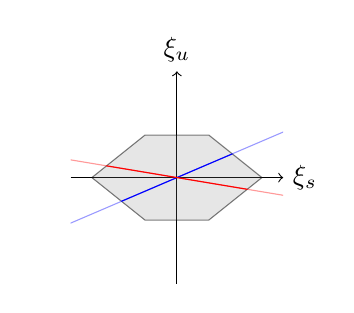
\begin{tikzpicture}[scale = 0.27]
	
		\draw[->] (-5, 0) -- (5, 0) node[right] {$\xi_s$};
		\draw[->] (0, -5) -- (0, 5) node[above] {$\xi_u$};
		
		% Invisible dummy node for symmetric alignment with caption
		\node[left, opacity = 0] at (-5, 0) {$\xi_s$};
		
		\draw[draw = black, fill = gray, fill opacity = 0.2, draw opacity = 0.5, name path = support_cut_off] (-4, 0) -- (-1.5, 2) -- (1.5, 2) -- (4, 0) -- (1.5, -2) -- (-1.5, -2) -- cycle;
		
		\begin{scope}
			\clip (-5, -5) rectangle (5, 5);
			\draw[scale = 1, smooth, domain = -10 : 10, variable = \x, blue, opacity = 0.4, name path = plane1] plot ({\x},{ -1 / (- 7 / 3) * \x});
			\draw[scale=1, smooth, domain = -10 : 10, variable = \x, red, opacity = 0.4, name path = plane2] plot ({\x},{ -1 / (12 / 2) * \x});
			
			\draw[blue, name intersections = {of = support_cut_off and plane1}] (intersection-1) -- (intersection-2);
			\draw[red, name intersections = {of = support_cut_off and plane2}] (intersection-1) -- (intersection-2);
			
		\end{scope}
		
	\end{tikzpicture}
	
\end{document}}
		\hspace{1cm}
		\subcaptionbox*{\centering Frequency Response (Amplitude)}{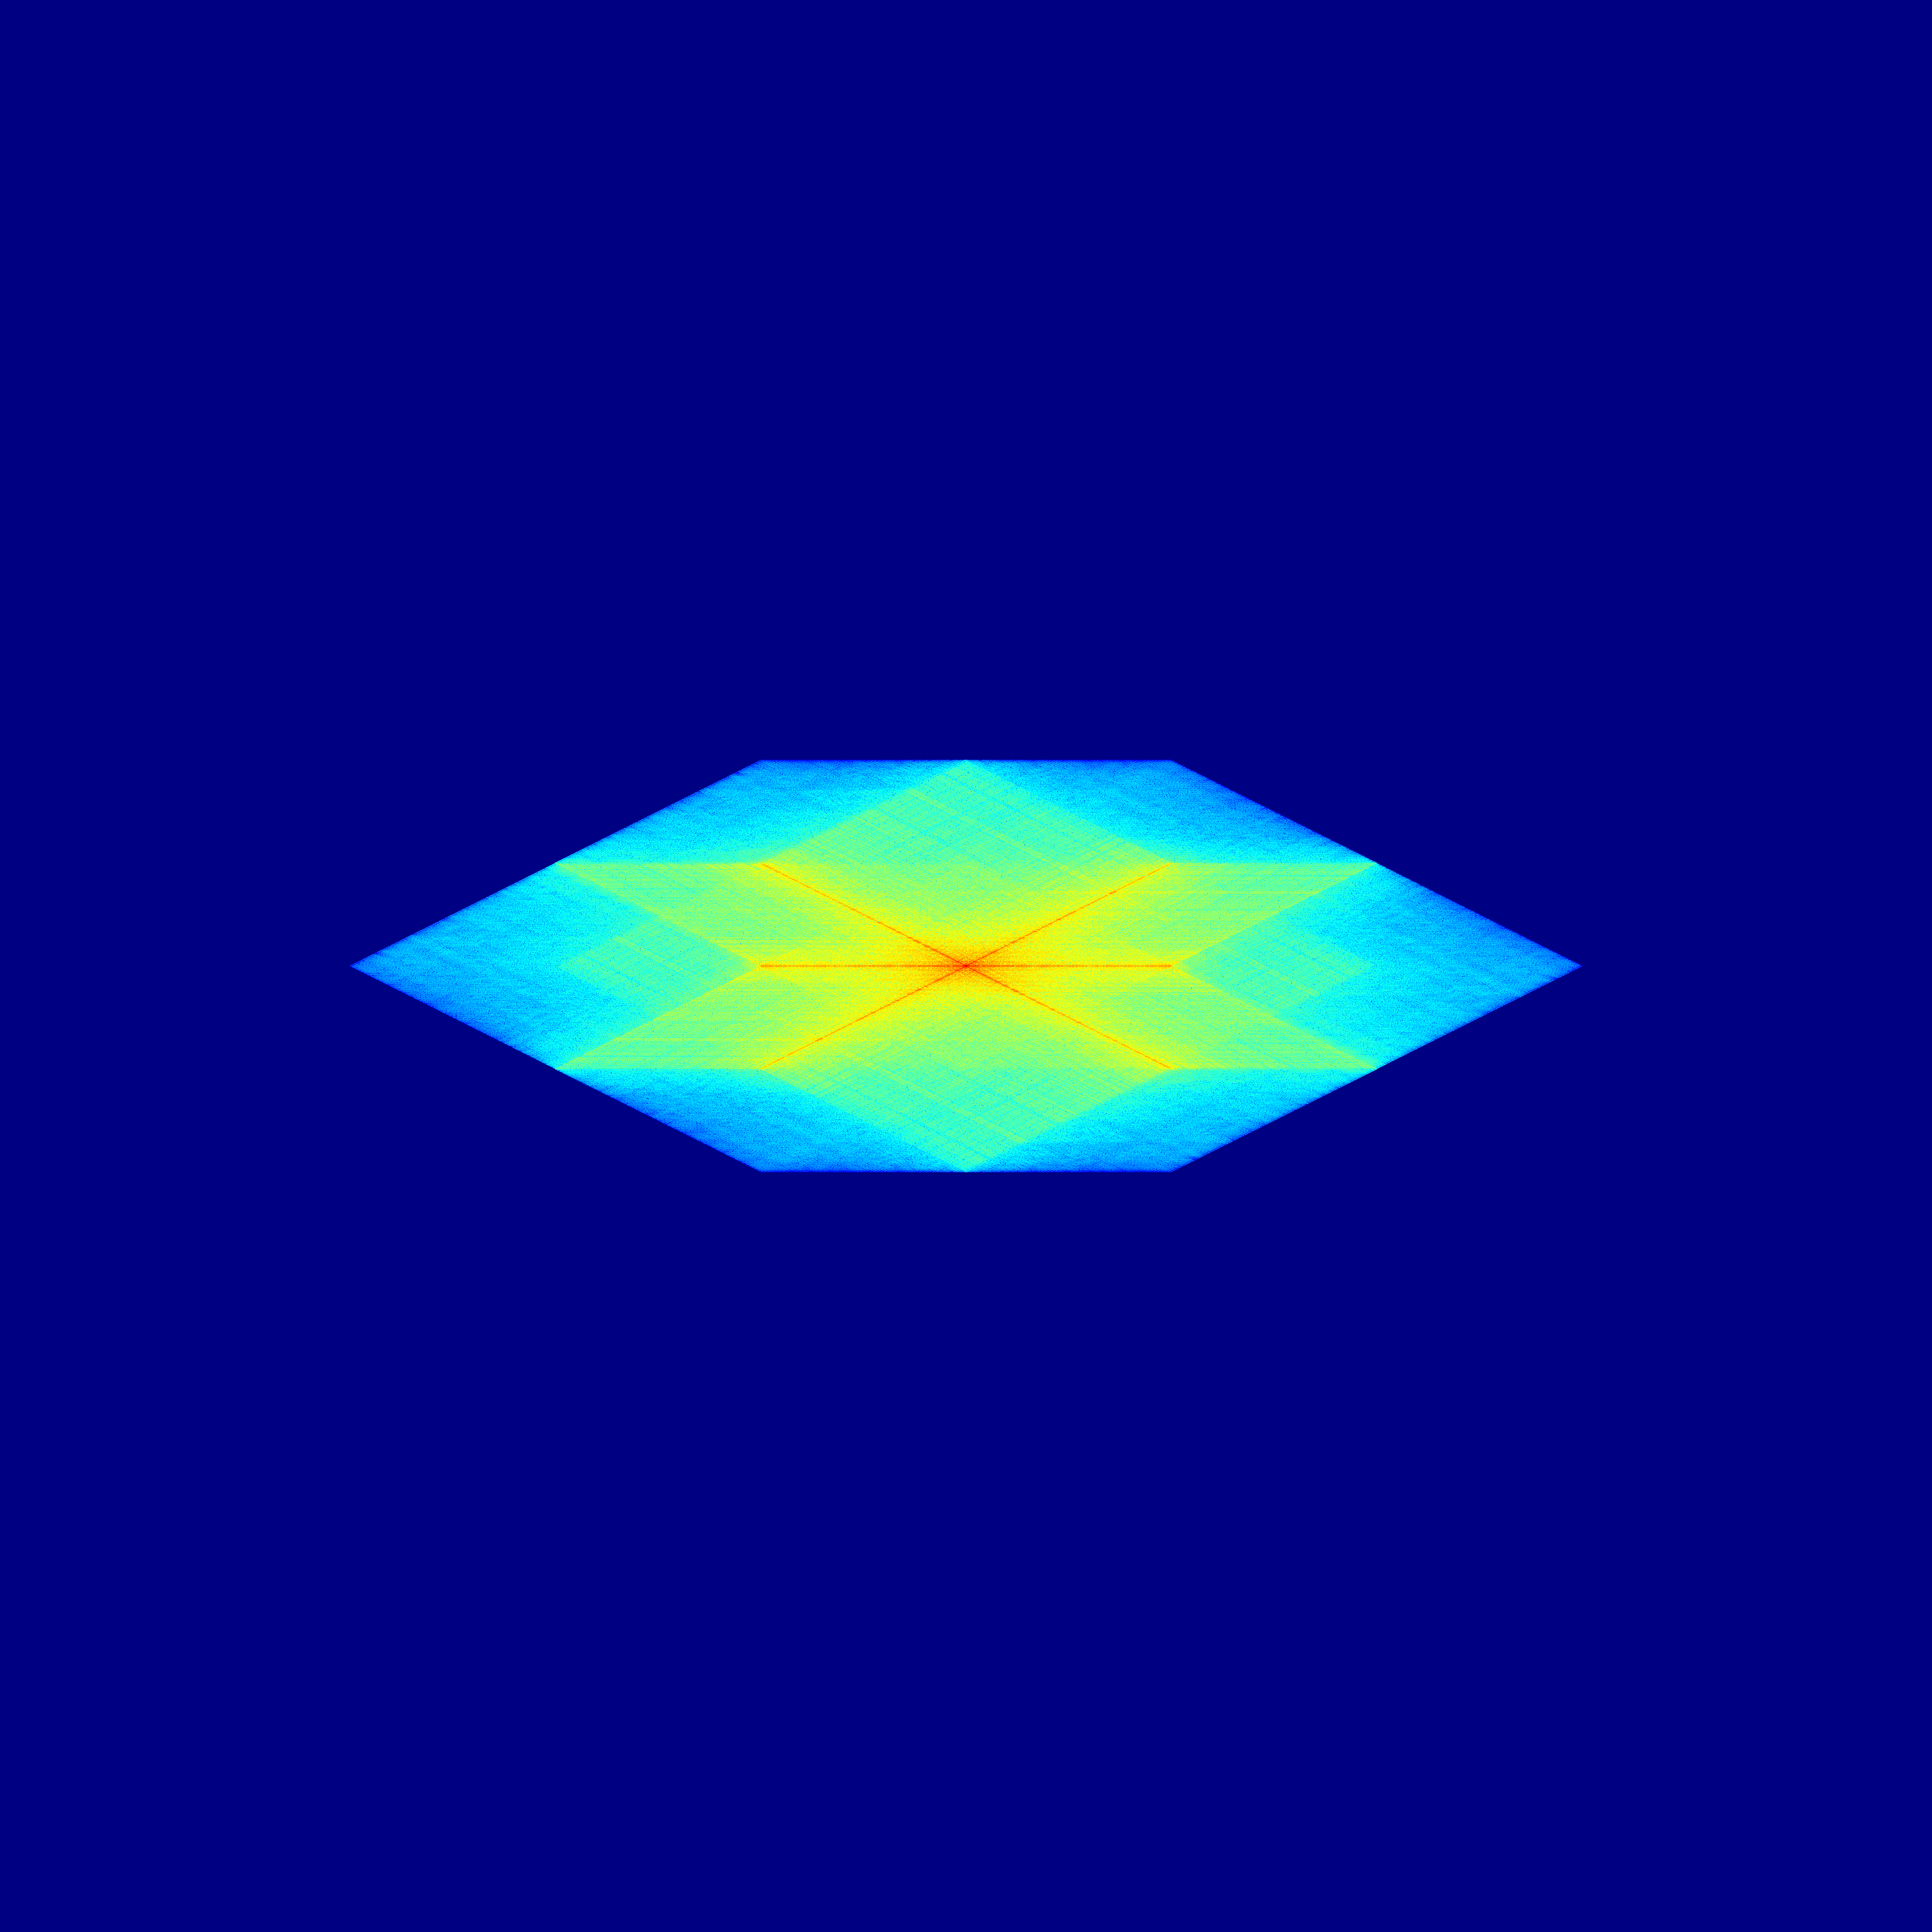
\includegraphics[height=4cm]{figures/spectral_support/convolution_3_layers}}
	\end{figure}
	
\end{frame}

\begin{frame}[fragile]
	\frametitle{Spectral Properties of Display}
	
	\begin{itemize}
		\item Spectral support increases with more layers
		\item Highest response in center
	\end{itemize}
	
	\begin{figure}
		\subcaptionbox*{2 Layers}{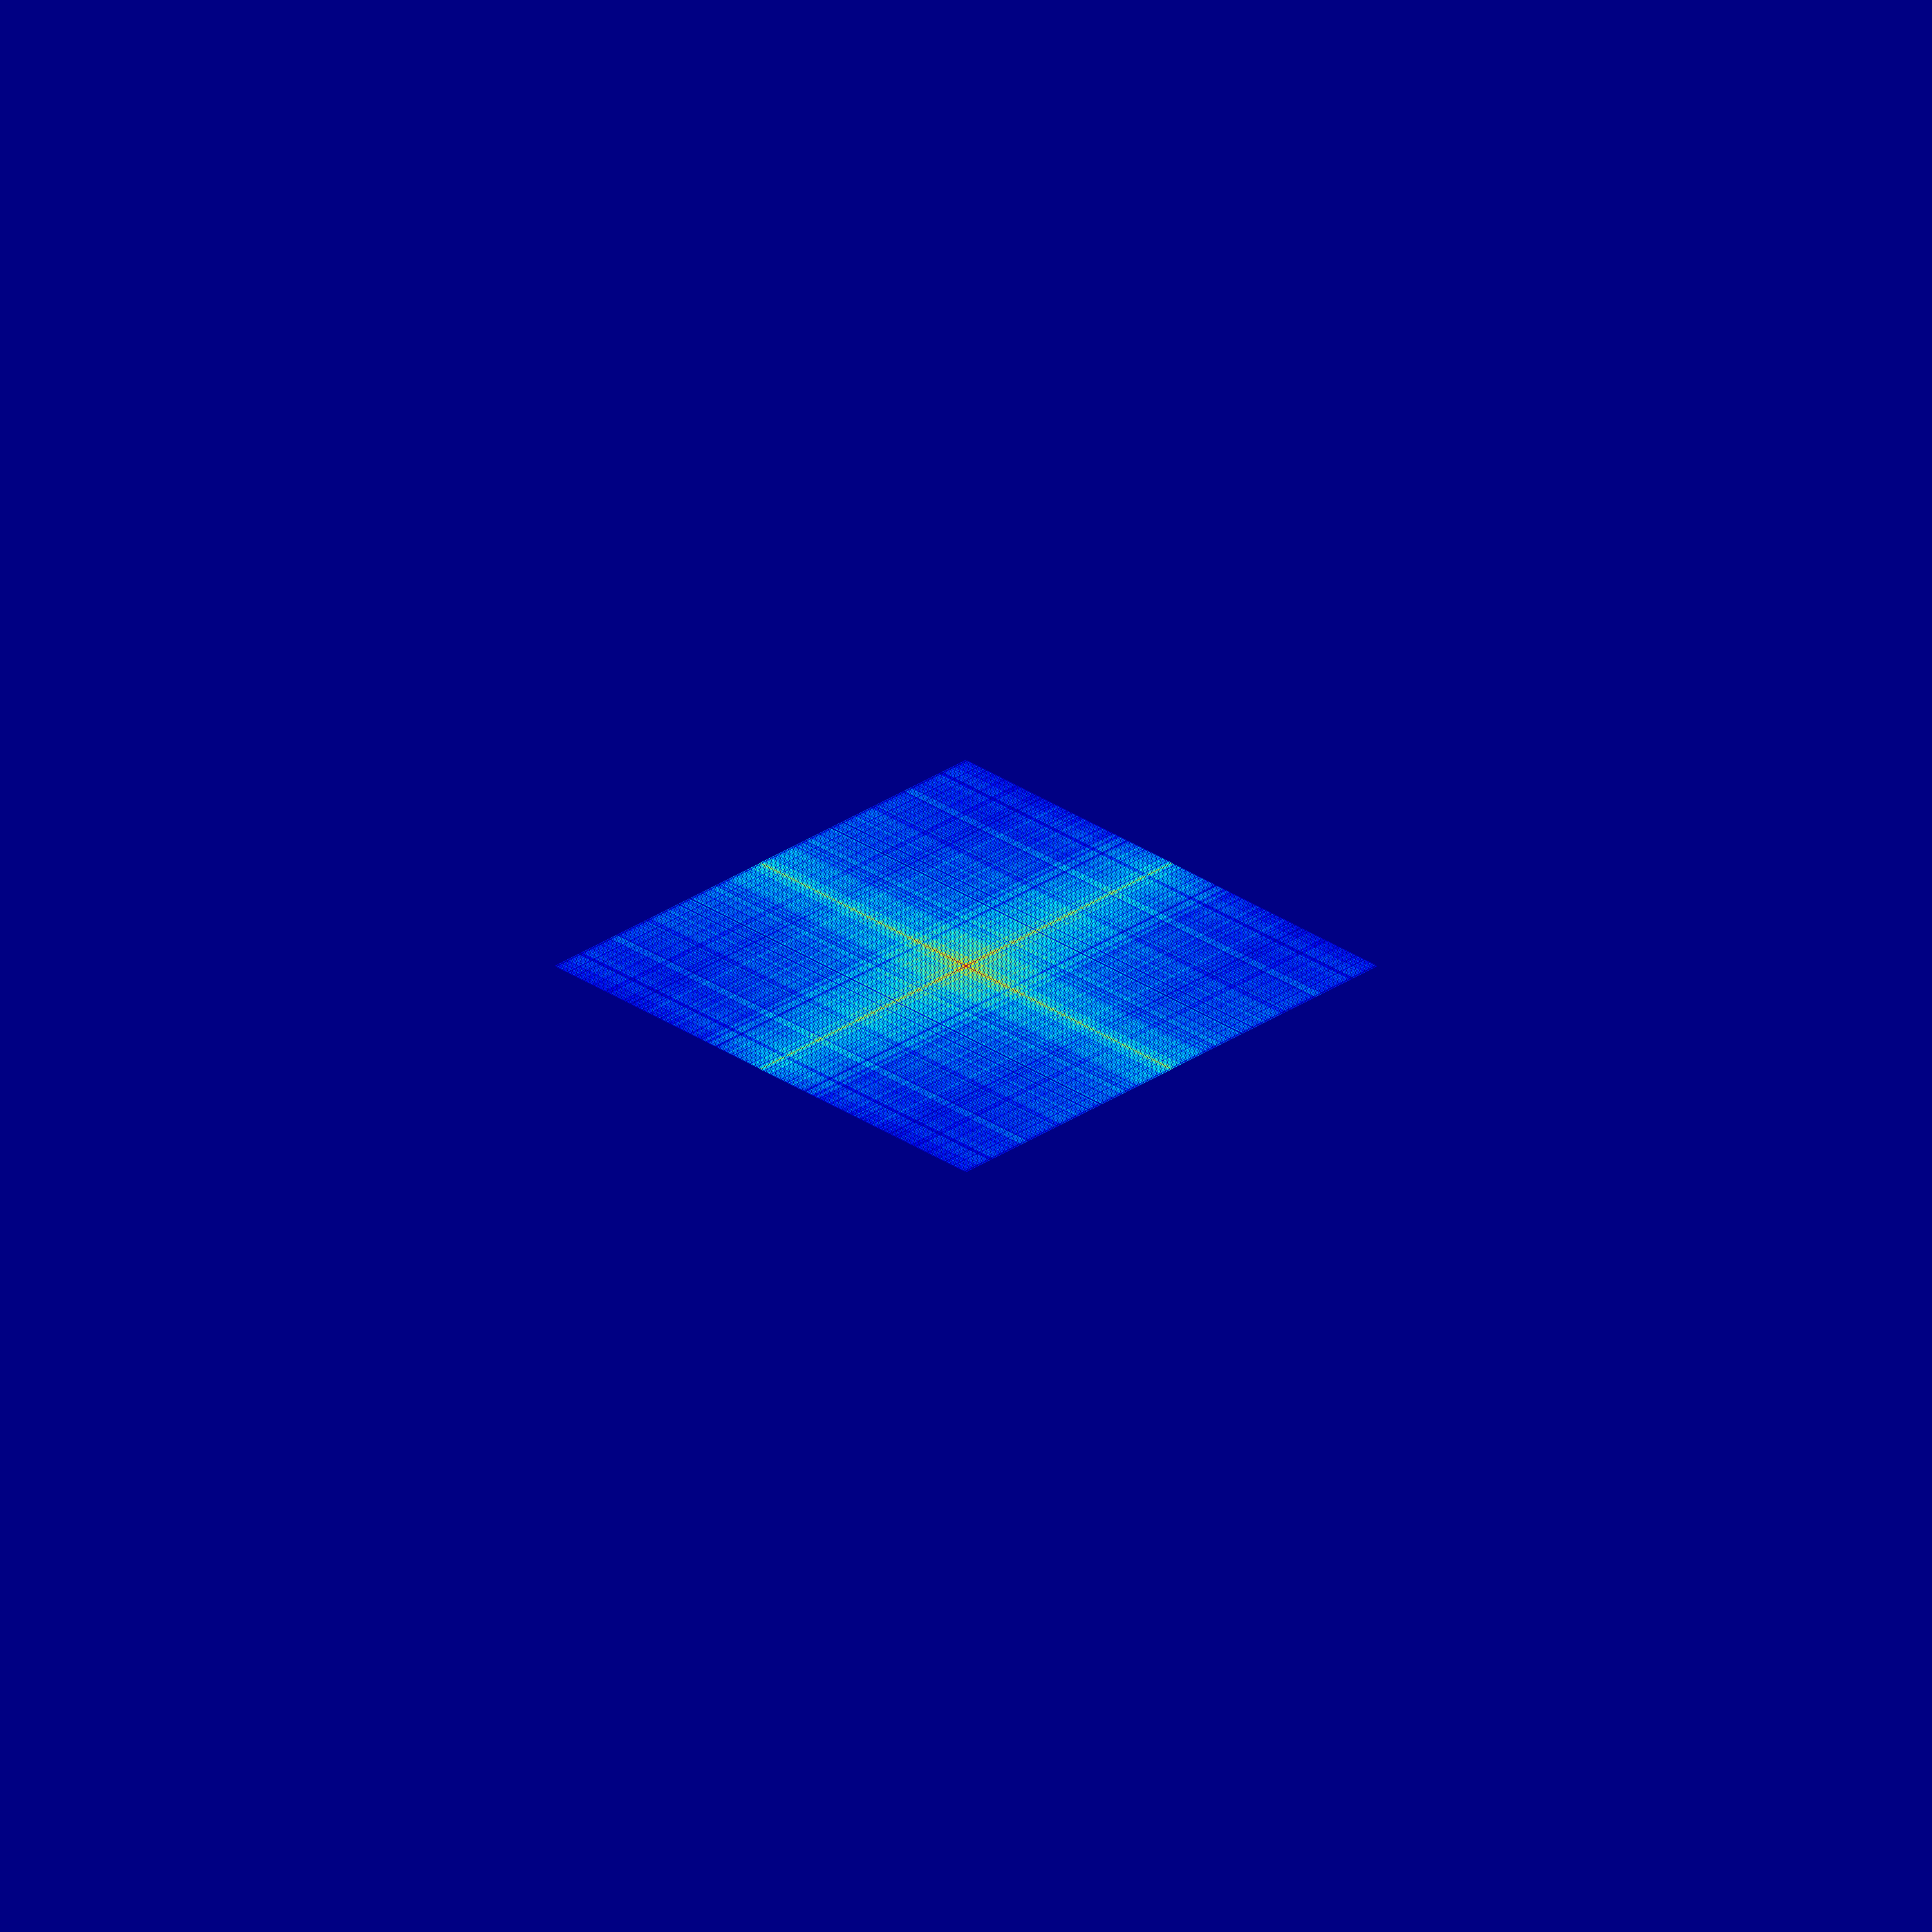
\includegraphics[height=3cm]{figures/spectral_support/convolution_2_layers}}
		\hspace{0.5cm}
		\subcaptionbox*{3 Layers}{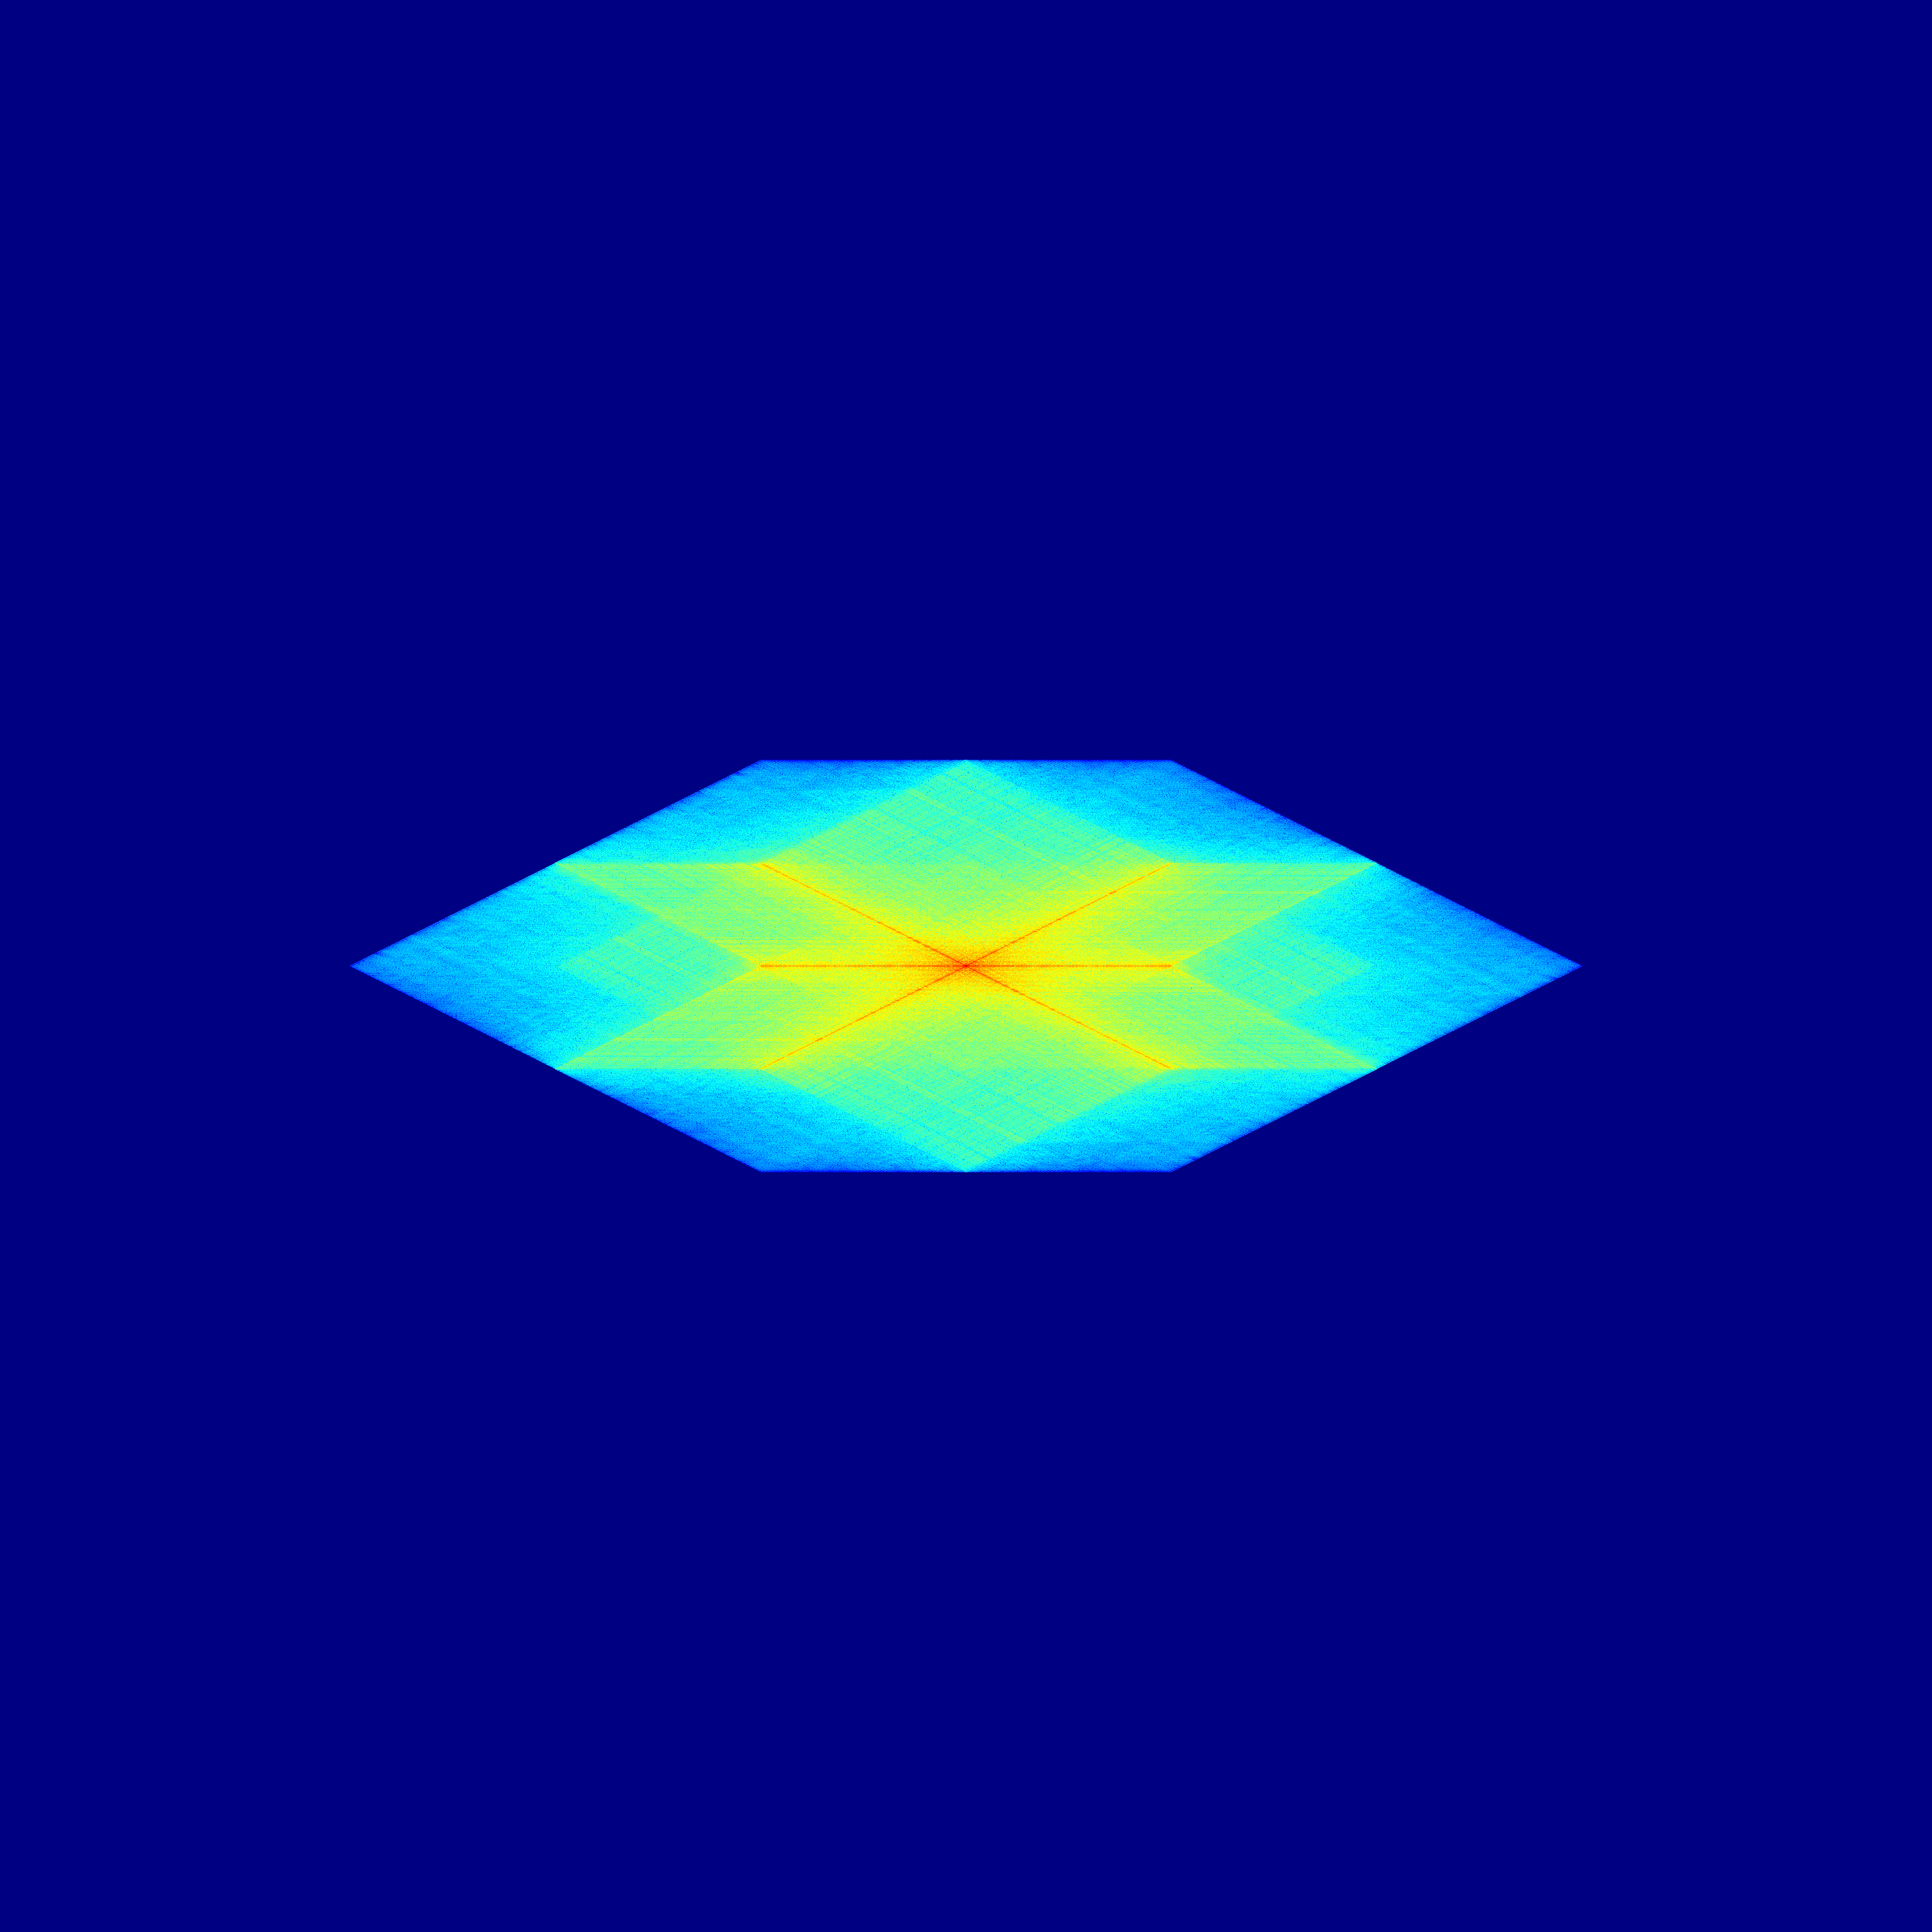
\includegraphics[height=3cm]{figures/spectral_support/convolution_3_layers}}
		\hspace{0.5cm}
		\subcaptionbox*{5 Layers}{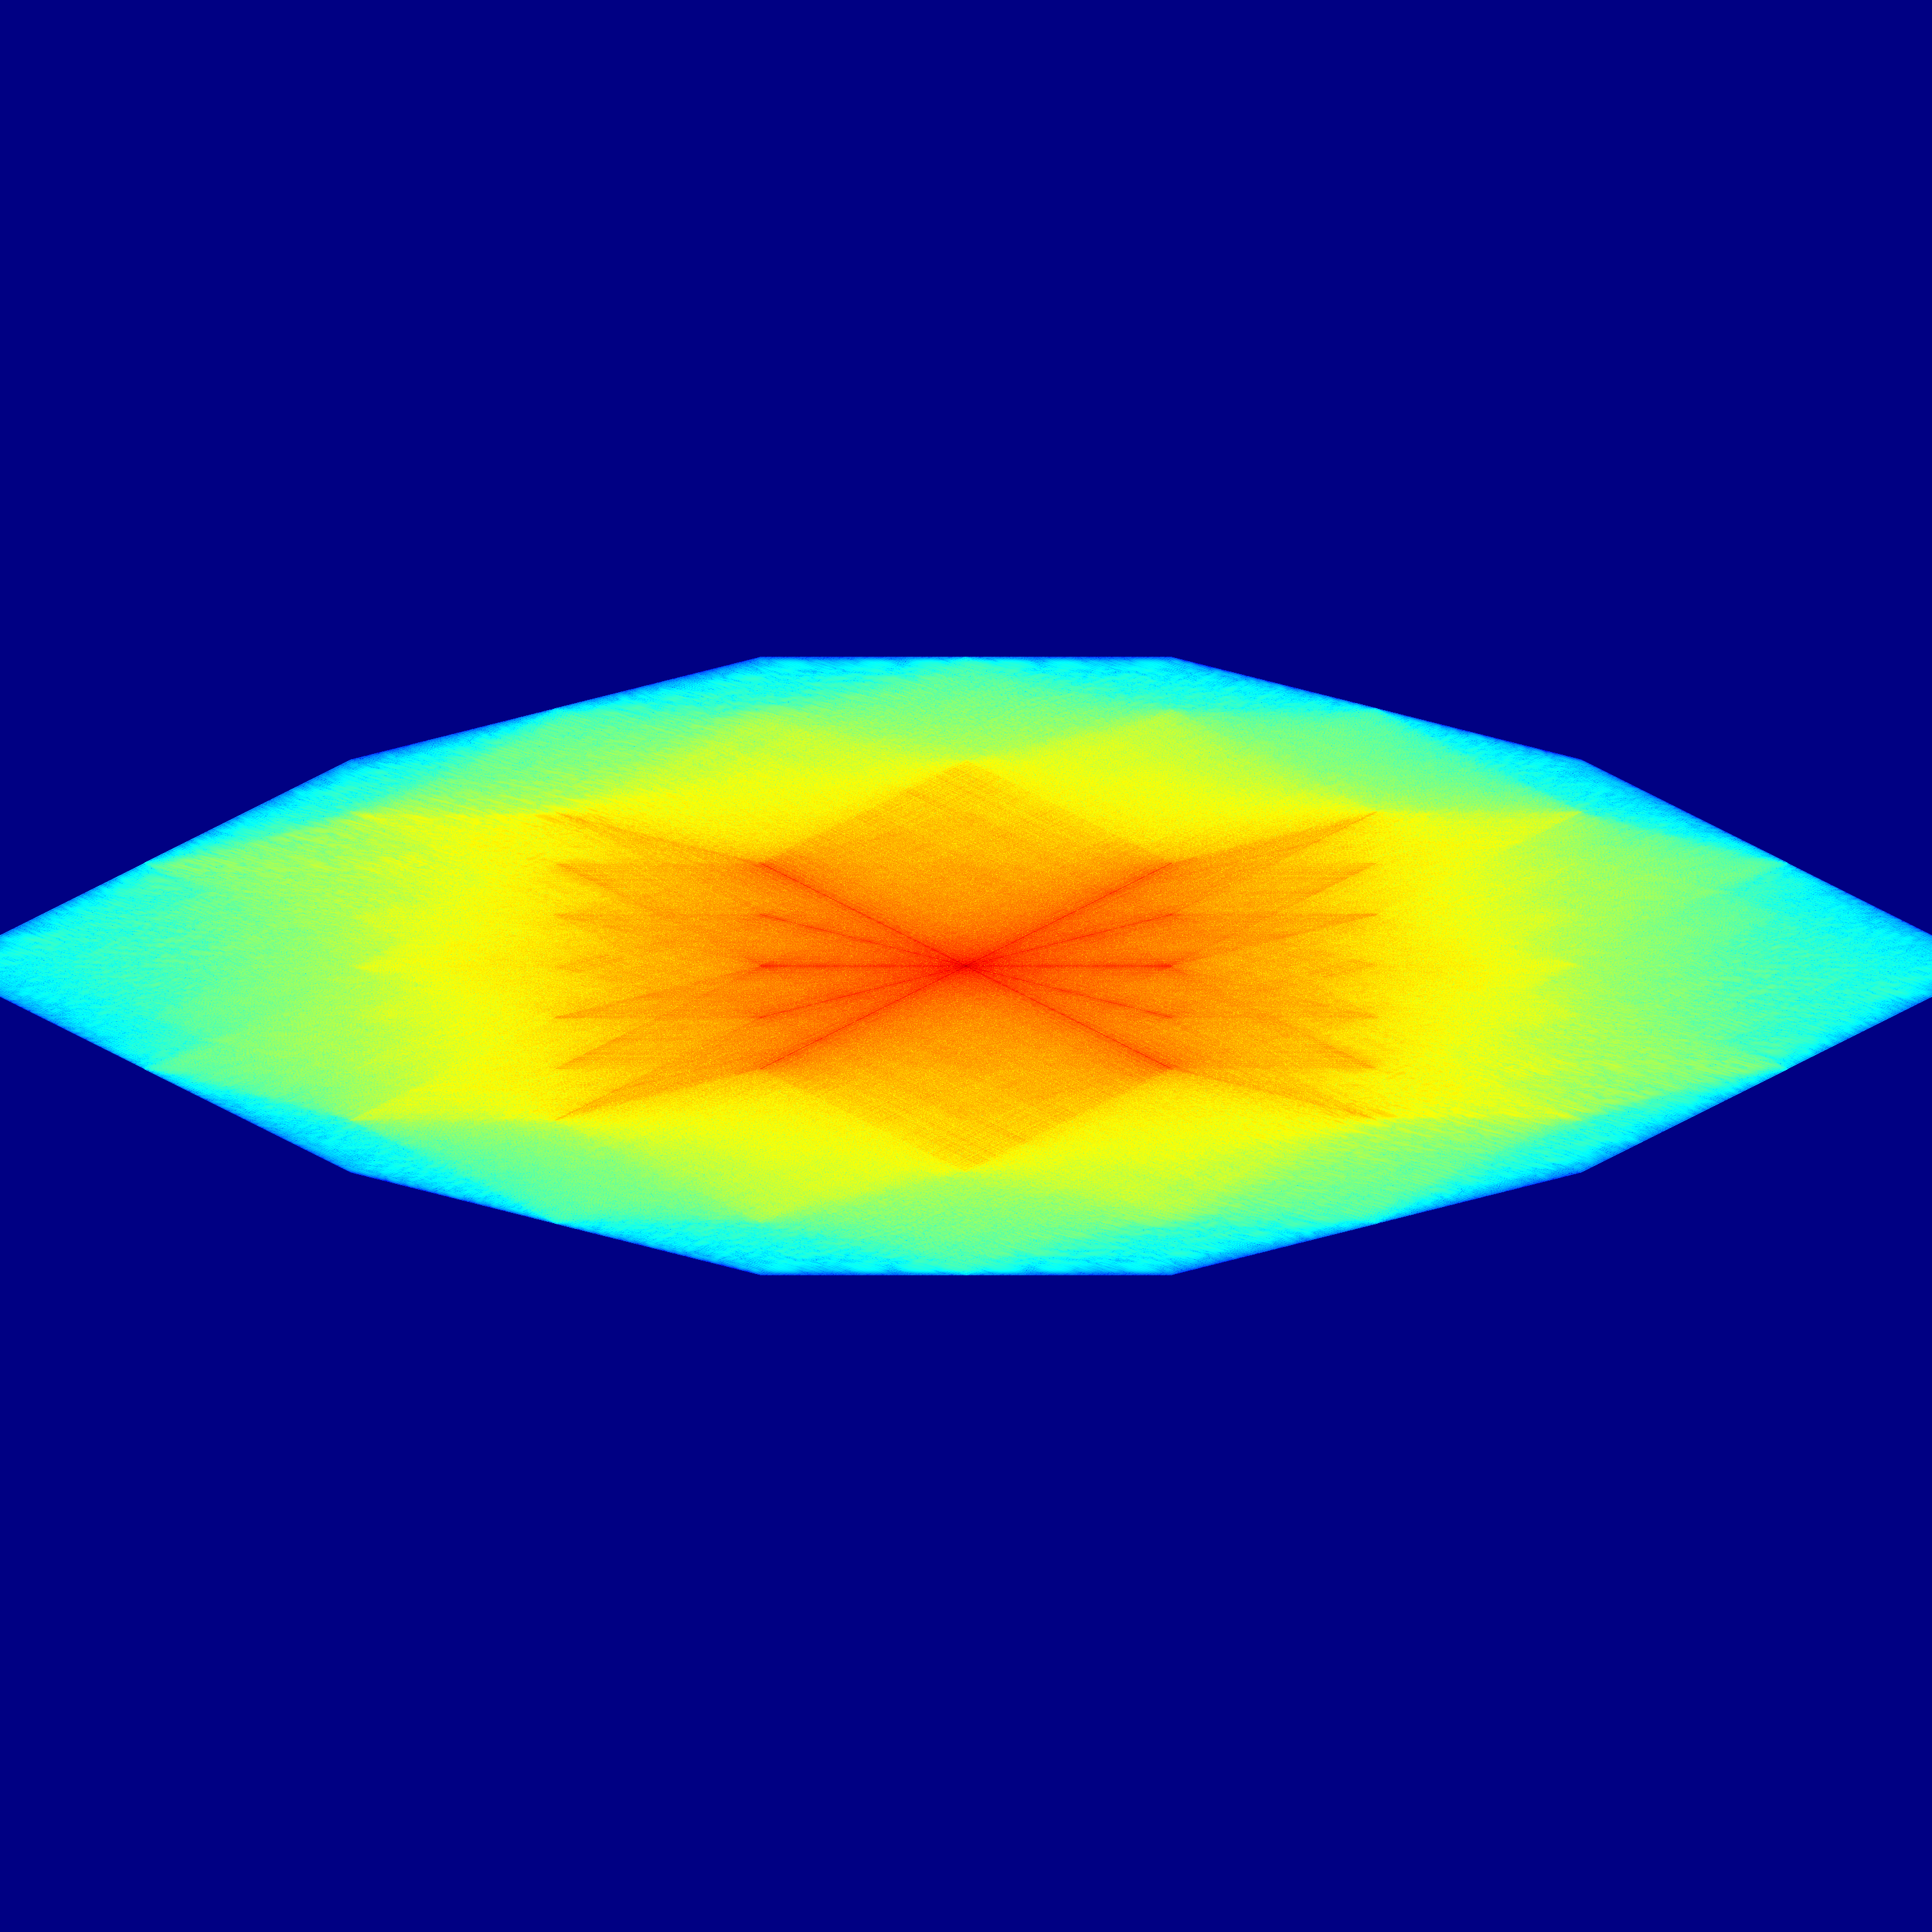
\includegraphics[height=3cm]{figures/spectral_support/convolution_5_layers}}
	\end{figure}
	
\end{frame}

\begin{frame}[fragile]
	\frametitle{Depth of Field}
	
	\begin{figure}
		\documentclass{standalone}
\usepackage{pgfplots}

\begin{document}
	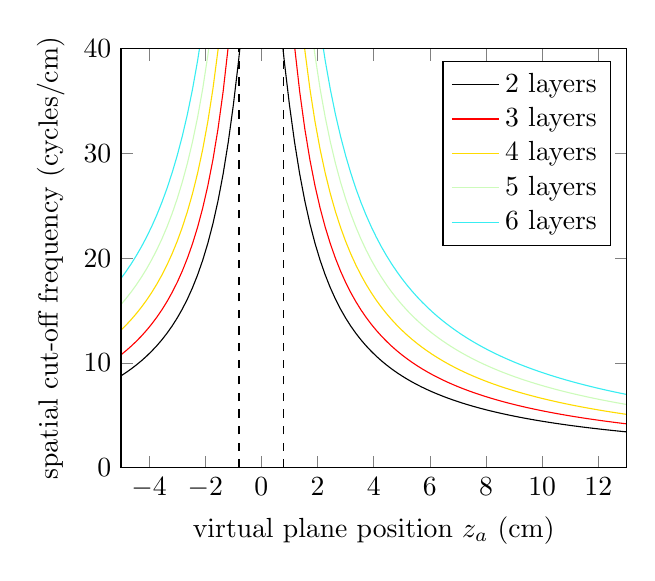
\begin{tikzpicture}
	
		\definecolor{c1}{RGB}{255, 0, 0}
		\definecolor{c2}{RGB}{255, 219, 0}
		\definecolor{c3}{RGB}{205, 251, 187}
		\definecolor{c4}{RGB}{56, 237, 242}
		\definecolor{c5}{RGB}{179, 46, 255}
	
		\pgfplotscreateplotcyclelist{mycolors}{black, c1, c2, c3, c4, c5}
		
		\begin{axis}[	legend pos = north east, 
						ymin = 0,
						ymax = 40, 
						xmin = -5,
						xmax = 13,
						domain = -5 : 13,
						xtick = {-4, -2, 0, 2, 4, 6, 8, 10, 12},
						ylabel = {spatial cut-off frequency (cycles/cm)},
						xlabel = {virtual plane position $z_a$ (cm)},
						ylabel near ticks,
						no markers,
						samples = 100, 
						cycle list name = mycolors,
						axis on top = true,
						width = 8 cm]
		
			% f_0 = 27.7 cycles/cm
			% h = 1.6 cm
		
			\addplot{2 * 27.7 * sqrt( (2 + 1) * 1.6^2 / ( (2 + 1) * 1.6^2 + 12 * (2 - 1) * (x^2) ) )};
			\addlegendentry{2 layers};
			
			\addplot{3 * 27.7 * sqrt( (3 + 1) * 1.6^2 / ( (3 + 1) * 1.6^2 + 12 * (3 - 1) * (x^2) ) )};
			\addlegendentry{3 layers};
			
			\addplot{4 * 27.7 * sqrt( (4 + 1) * 1.6^2 / ( (4 + 1) * 1.6^2 + 12 * (4 - 1) * (x^2) ) )};
			\addlegendentry{4 layers};
			
			\addplot{5 * 27.7 * sqrt( (5 + 1) * 1.6^2 / ( (5 + 1) * 1.6^2 + 12 * (5 - 1) * (x^2) ) )};
			\addlegendentry{5 layers};
			
			\addplot{6 * 27.7 * sqrt( (6 + 1) * 1.6^2 / ( (6 + 1) * 1.6^2 + 12 * (6 - 1) * (x^2) ) )};
			\addlegendentry{6 layers};
			
			\addplot[dashed] coordinates {(-0.8, 0) (-0.8, 100)};
			\addplot[dashed] coordinates {(0.8, 0) (0.8, 100)};
			 
		\end{axis}
		
	\end{tikzpicture}
\end{document}
	\end{figure}
\end{frame}

%\begin{frame}[fragile]
%	\frametitle{Depth of Field}
%	
%	\begin{figure}
%		\documentclass{standalone}
\usepackage{pgfplots}

\begin{document}
	\begin{tikzpicture}
	
		\definecolor{c1}{RGB}{255, 0, 0}
		\definecolor{c2}{RGB}{255, 0, 0}
		\definecolor{c3}{RGB}{255, 0, 0}
		\definecolor{c4}{RGB}{255, 0, 0}
		\definecolor{c5}{RGB}{255, 0, 0}
	
		\pgfplotscreateplotcyclelist{mycolors}{c1, c2, c3, c5, c4, c5, c4}
		
		\begin{axis}[	legend pos = north east, 
						ymin = 0,
						ymax = 50, 
						xmin = -5,
						xmax = 11,
						domain = -5 : 13,
						xtick = {-4, -2, 0, 2, 4, 6, 8, 10, 12},
						ylabel = {spatial cut-off frequency (cycles/cm)},
						xlabel = {virtual plane position $z_a$ (cm)},
						ylabel near ticks,
						no markers,
						samples = 150, 
						cycle list name = mycolors,
						axis on top = true,
						width = 8 cm, 
						height = 8 cm]
		
			% f_0 = 27.7 cycles/cm
			% h = 1.6 cm
		\only<1,2,3,4,5>{
			\addplot{2 * 27.7 * sqrt( (2 + 1) * 1.6^2 / ( (2 + 1) * 1.6^2 + 12 * (2 - 1) * (x^2) ) )};
%			\addlegendentry{2 layers};
		}
		\only<2,3,4,5>{
			\addplot{3 * 27.7 * sqrt( (3 + 1) * 1.6^2 / ( (3 + 1) * 1.6^2 + 12 * (3 - 1) * (x^2) ) )};
%			\addlegendentry{3 layers};
		}
			
		\only<3,4,5>{
			\addplot{4 * 27.7 * sqrt( (4 + 1) * 1.6^2 / ( (4 + 1) * 1.6^2 + 12 * (4 - 1) * (x^2) ) )};
%			\addlegendentry{4 layers};
		}
			
		\only<4,5>{
			\addplot{5 * 27.7 * sqrt( (5 + 1) * 1.6^2 / ( (5 + 1) * 1.6^2 + 12 * (5 - 1) * (x^2) ) )};
%			\addlegendentry{5 layers};
		}
			
		\only<5>{
			\addplot{6 * 27.7 * sqrt( (6 + 1) * 1.6^2 / ( (6 + 1) * 1.6^2 + 12 * (6 - 1) * (x^2) ) )};
%			\addlegendentry{6 layers};
		}
		
%			\addplot[dashed, cap = round, c1]{27.7 * sqrt( 2 * (2 * 2 - 1) * 1.6^2 / ( (2 + 1) * 1.6^2 + 12 * (2 - 1) * (x^2) ) )};
%			\addlegendentry{2 layers};
			
%			\addplot[dotted, cap = round, c2]{27.7 * sqrt( 2 * (2 * 3 - 1) * 1.6^2 / ( (3 + 1) * 1.6^2 + 12 * (3 - 1) * (x^2) ) )};
%			\addplot[dotted, cap = round, c3]{27.7 * sqrt( 2 * (2 * 4 - 1) * 1.6^2 / ( (4 + 1) * 1.6^2 + 12 * (4 - 1) * (x^2) ) )};
%			\addplot[dotted, cap = round, c4]{27.7 * sqrt( 2 * (2 * 5 - 1) * 1.6^2 / ( (5 + 1) * 1.6^2 + 12 * (5 - 1) * (x^2) ) )};
			
%			\addplot[dashed, cap = round, c4]{27.7 * sqrt( 2 * (2 * 6 - 1) * 1.6^2 / ( (6 + 1) * 1.6^2 + 12 * (6 - 1) * (x^2) ) )};
%			\addlegendentry{6 layers};
			
			\addplot[dashed] coordinates {(-0.8, 0) (-0.8, 100)};
			\addplot[dashed] coordinates {(0.8, 0) (0.8, 100)};
			
		\end{axis}
		
	\end{tikzpicture}
\end{document}
%	\end{figure}
%\end{frame}

\begin{frame}[fragile]
	\frametitle{Display Thickness}
	
	\begin{figure}
		\subcaptionbox*{Original}{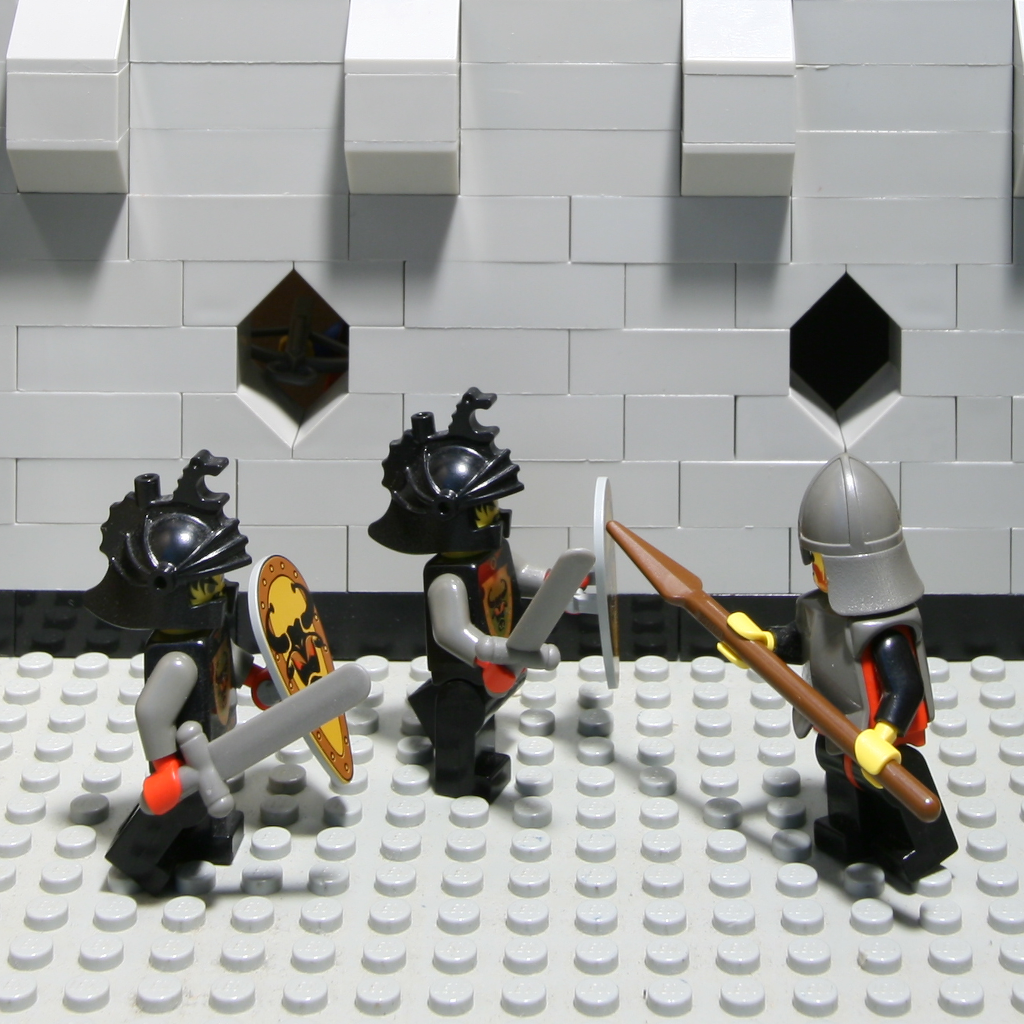
\includegraphics[height=5cm]{figures/depth_of_field/original_08_08}}
		\hspace{0.5cm}
		\subcaptionbox*{16 mm thick}{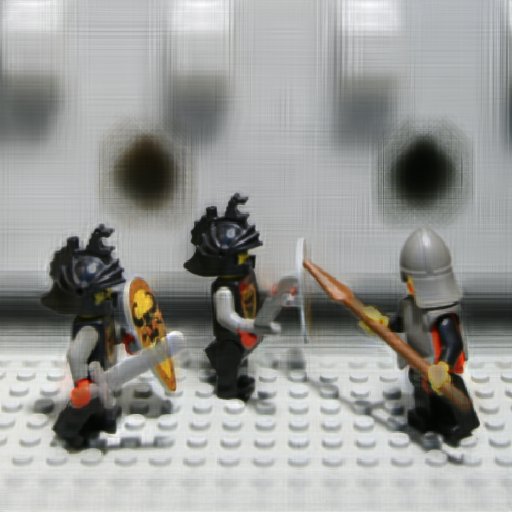
\includegraphics[height=5cm]{figures/depth_of_field/knights_thickness_16mm/Reconstruction_of_view_(5,5)}}
	\end{figure}
	
	{\scriptsize Light field courtesy: \href{http://lightfield.stanford.edu/lfs.html}{Stanford Light Field Archive}}
\end{frame}

\begin{frame}[fragile]
	\frametitle{Display Thickness}
	
	\begin{figure}
		\subcaptionbox*{Original}{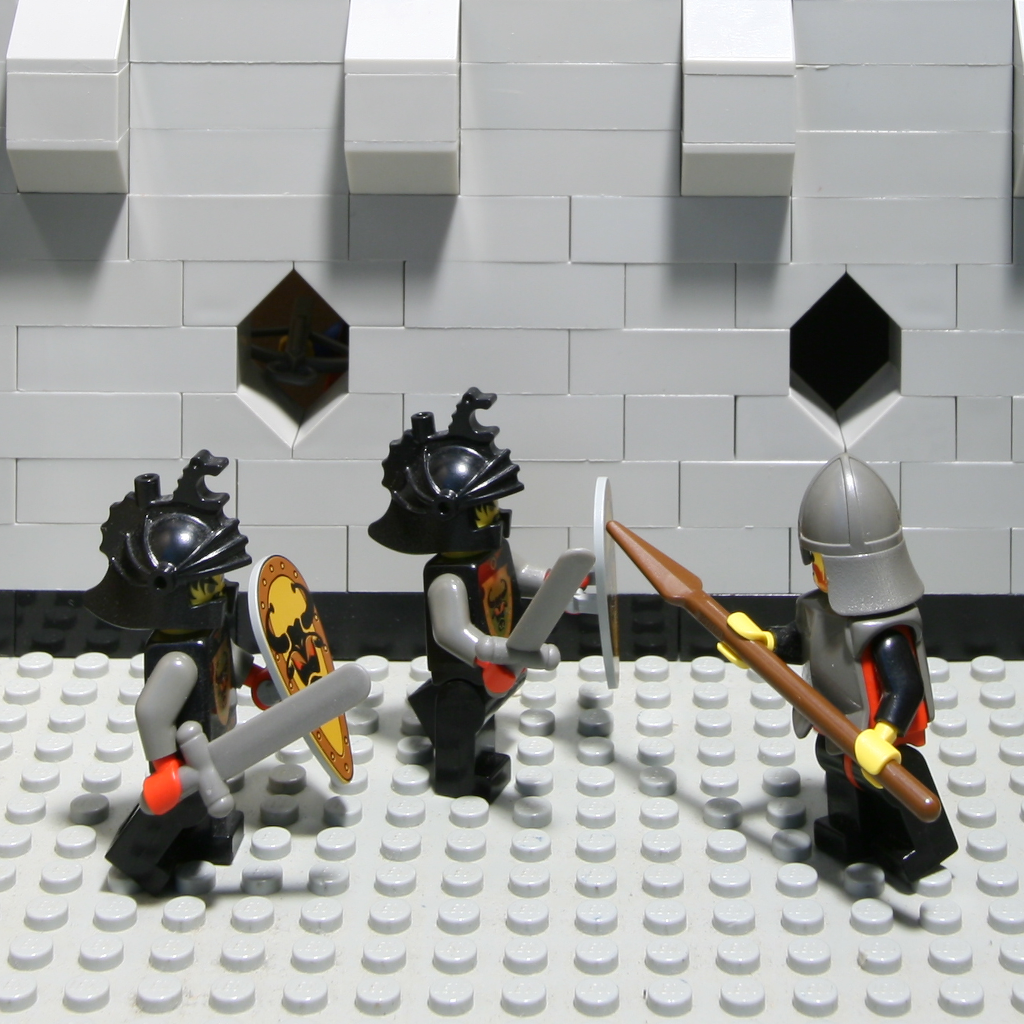
\includegraphics[height=5cm]{figures/depth_of_field/original_08_08}}
		\hspace{0.5cm}
		\subcaptionbox*{30 mm thick}{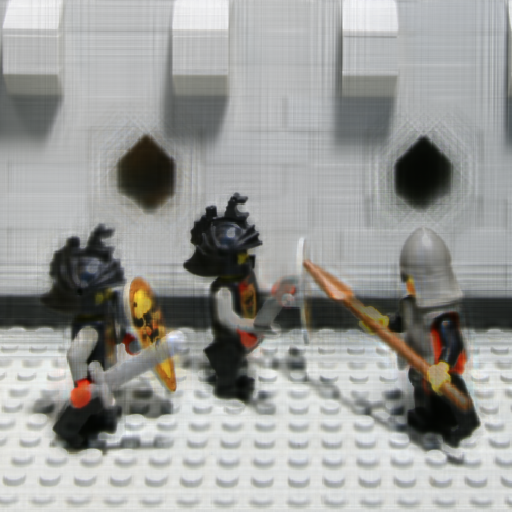
\includegraphics[height=5cm]{figures/depth_of_field/knights_thickness_30mm/Reconstruction_of_view_(5,5)}}
	\end{figure}
	
	{\scriptsize Light field courtesy: \href{http://lightfield.stanford.edu/lfs.html}{Stanford Light Field Archive}}
\end{frame}

\section{Conclusion}

\begin{frame}[fragile]
	\frametitle{The Good}
	
	\begin{itemize}
		\item \alert<1>{No trade-off between angular- and spatial resolution}
		\item \alert<2>{Extended spectral support}
		\item \alert<3>{Works with different types of light fields}
		\begin{itemize}
			\item Oblique Projections (synthetic scenes)
			\item Perspective Projections (cameras)
			\item Lytro
		\end{itemize}
	\end{itemize}
\end{frame}

\begin{frame}[fragile]
	\frametitle{The Bad}
	
	\begin{itemize}
		\item \alert<1>{Very small viewing angles}
		\item \alert<2>{Depth of field highly dependent on thickness}
		\begin{itemize}
			\item Light field's depth of field needs to match
			\item For fixed thickness, need to adjust baseline
		\end{itemize}
		\item \alert<3>{Need many layers to eliminate halo artifacts}
		\item \alert<4>{Manual layer alignment is hard}
	\end{itemize}
\end{frame}

\begin{frame}
	\begin{center}
		\LARGE Your Questions
	\end{center}
\end{frame}

\begin{frame}
	\frametitle{Acknowledgements}
	
	\begin{block}{Supervision by}
		Prof. Dr. Matthias Zwicker \\
		Siavash Bigdeli
	\end{block}
\end{frame}

\begin{frame}[fragile]
	\frametitle{More Information}
	
	\begin{block}{Contact}
  		adrian.waelchli@students.unibe.ch
	\end{block}
	
	\begin{block}{Thesis and Resources}
		\href{https://github.com/awaelchli/bachelor_thesis}{github.com/awaelchli/bachelor\_thesis}
	\end{block}
\end{frame}

\begin{frame}<beamer:0>
	\frametitle{References}
	
	\bibliographystyle{abbrvnat}
%	\bibliographystyle{apalike}
	\def\bibfont{\scriptsize}
	%\nocite{*}
	\bibliography{presentation}
\end{frame}

% % % % % % % % % % % % % % %
% HIDDEN SLIDES % % % % % % %
% % % % % % % % % % % % % % %

\begin{frame}
	\begin{center}
		\LARGE Hidden Slides
	\end{center}
\end{frame}

\begin{frame}[fragile]
	\frametitle{Re-Parameterization to Global Coordinates}
	
	\begin{center}
		\visible<1,2>{\documentclass{standalone}
\usepackage{tikz}

\begin{document}
	
	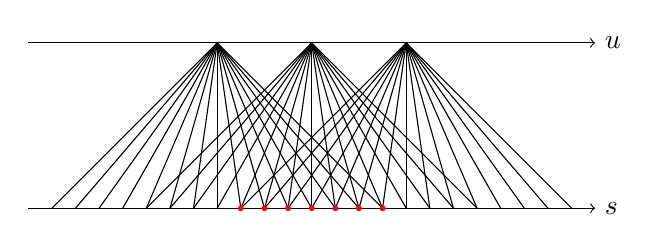
\begin{tikzpicture}[scale = 0.3]
		
		\draw[->] (-9, 0) -- (15, 0);
		\draw[->] (-9, 7) -- (15, 7);
		
		\node[right] at (15, 0) {$s$};
		\node[right] at (15, 7) {$u$};
		
		\draw (-1, 7) -- (-8, 0);
		\draw (-1, 7) -- (-7, 0);
		\draw (-1, 7) -- (-6, 0);
		\draw (-1, 7) -- (-5, 0);
		\draw (-1, 7) -- (-4, 0);
		\draw (-1, 7) -- (-3, 0);
		\draw (-1, 7) -- (-2, 0);
		\draw (-1, 7) -- (-1, 0);
		\draw (-1, 7) -- (0, 0);
		\draw (-1, 7) -- (1, 0);
		\draw (-1, 7) -- (2, 0);
		\draw (-1, 7) -- (3, 0);
		\draw (-1, 7) -- (4, 0);
		\draw (-1, 7) -- (5, 0);
		\draw (-1, 7) -- (6, 0);
		
		\draw (3, 7) -- (-4, 0);
		\draw (3, 7) -- (-3, 0);
		\draw (3, 7) -- (-2, 0);
		\draw (3, 7) -- (-1, 0);
		\draw (3, 7) -- (0, 0);
		\draw (3, 7) -- (1, 0);
		\draw (3, 7) -- (2, 0);
		\draw (3, 7) -- (3, 0);
		\draw (3, 7) -- (4, 0);
		\draw (3, 7) -- (5, 0);
		\draw (3, 7) -- (6, 0);
		\draw (3, 7) -- (7, 0);
		\draw (3, 7) -- (8, 0);
		\draw (3, 7) -- (9, 0);
		\draw (3, 7) -- (10, 0);
		
		\draw (7, 7) -- (0, 0);
		\draw (7, 7) -- (1, 0);
		\draw (7, 7) -- (2, 0);
		\draw (7, 7) -- (3, 0);
		\draw (7, 7) -- (4, 0);
		\draw (7, 7) -- (5, 0);
		\draw (7, 7) -- (6, 0);
		\draw (7, 7) -- (7, 0);
		\draw (7, 7) -- (8, 0);
		\draw (7, 7) -- (9, 0);
		\draw (7, 7) -- (10, 0);
		\draw (7, 7) -- (11, 0);
		\draw (7, 7) -- (12, 0);
		\draw (7, 7) -- (13, 0);
		\draw (7, 7) -- (14, 0);
		
		\draw[fill, red] (0, 0) circle [radius = 0.1];
		\draw[fill, red] (1, 0) circle [radius = 0.1];
		\draw[fill, red] (2, 0) circle [radius = 0.1];
		\draw[fill, red] (3, 0) circle [radius = 0.1];
		\draw[fill, red] (4, 0) circle [radius = 0.1];
		\draw[fill, red] (5, 0) circle [radius = 0.1];
		\draw[fill, red] (6, 0) circle [radius = 0.1];
	\end{tikzpicture}
	
\end{document}}
		\visible<2>{
			
\begin{tikzpicture}
				\draw[->, red, line width = 0.075cm] (0, 0) -- (0, -0.7);
			\end{tikzpicture}
		}	
		\visible<2>{\documentclass{standalone}
\usepackage{tikz}

\begin{document}
	
	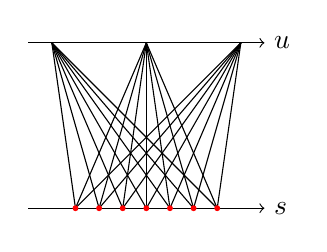
\begin{tikzpicture}[scale = 0.3]
		
		\draw[->] (-2, 0) -- (8, 0);
		\draw[->] (-2, 7) -- (8, 7);
		
		\node[right] at (8, 0) {$s$};
		\node[right] at (8, 7) {$u$};
		
		\draw (-1, 7) -- (0, 0);
		\draw (-1, 7) -- (1, 0);
		\draw (-1, 7) -- (2, 0);
		\draw (-1, 7) -- (3, 0);
		\draw (-1, 7) -- (4, 0);
		\draw (-1, 7) -- (5, 0);
		\draw (-1, 7) -- (6, 0);
		
		\draw (3, 7) -- (0, 0);
		\draw (3, 7) -- (1, 0);
		\draw (3, 7) -- (2, 0);
		\draw (3, 7) -- (3, 0);
		\draw (3, 7) -- (4, 0);
		\draw (3, 7) -- (5, 0);
		\draw (3, 7) -- (6, 0);
		
		\draw (7, 7) -- (0, 0);
		\draw (7, 7) -- (1, 0);
		\draw (7, 7) -- (2, 0);
		\draw (7, 7) -- (3, 0);
		\draw (7, 7) -- (4, 0);
		\draw (7, 7) -- (5, 0);
		\draw (7, 7) -- (6, 0);
		
		\draw[fill, red] (0, 0) circle [radius = 0.1];
		\draw[fill, red] (1, 0) circle [radius = 0.1];
		\draw[fill, red] (2, 0) circle [radius = 0.1];
		\draw[fill, red] (3, 0) circle [radius = 0.1];
		\draw[fill, red] (4, 0) circle [radius = 0.1];
		\draw[fill, red] (5, 0) circle [radius = 0.1];
		\draw[fill, red] (6, 0) circle [radius = 0.1];
		
	\end{tikzpicture}
	
\end{document}}
	\end{center}
\end{frame}

\begin{frame}[fragile]
	\frametitle{Re-Parameterization to Global Coordinates}
	
	\begin{center}
		\begin{tabular}{c p{0.5cm} c}
			Raw & & Rectified \\
			\fbox{\includegraphics[height=5cm]{images/rectification/dice000_raw}}
			& &\fbox{\includegraphics[height=5cm]{images/rectification/dice000_rectified}}
		\end{tabular}
	\end{center}
\end{frame}

\begin{frame}[fragile]
	\frametitle{Re-Parameterization to Global Coordinates}
	
	\begin{center}
		\begin{tabular}{c p{0.5cm} c}
			Raw & & Rectified \\
			\fbox{\includegraphics[height=5cm]{images/rectification/dice499_raw}}
			& &\fbox{\includegraphics[height=5cm]{images/rectification/dice499_rectified}}
		\end{tabular}
	\end{center}
\end{frame}

\begin{frame}[fragile]
	\frametitle{Ray Casting}
	$
		P = 
		\begin{blockarray}{lcccccccccc}
		    				& \alpha_1 	& \alpha_2 	& \alpha_3 	& \alpha_4 	& \alpha_5 	& \alpha_6 	& \alpha_7 	& \alpha_8 	& \alpha_9 	& \alpha_{10}	\\
		    \begin{block}{l(ccccc|ccccc@{\hspace*{5pt}})}
			  L_1 	& 	 		& 			& 	1		& 			& 			& 	1		&			&			&			&				\\
			  L_2 	& 			& 			& 			& 	1		& 			& 	1		&			&			&			&				\\
			  L_3 	& 	1		& 			& 			& 			& 			& 			&	1		&			&			&				\\
			  L_4 	& 			& 	1		& 			& 			& 			& 			&			&			&	1		&				\\
			  \cline{2-11}
			  L_5 	& 			& 			& 			& 			& 	1		& 			&			&			&	1		&				\\
			  L_6 	& 			& 			& 	1		& 			& 			& 1			&			&			&			&				\\
			  L_7 	& 		1	& 			& 			& 			& 			& 			&			&			&	1		&				\\
			  L_8 	& 			& 			& 			& 	 		& 	1		& 			&	1		&			&			&				\\
			  \cline{2-11}
			  L_9 	& 			& 	1		& 			& 			& 			& 			&	1		&			& 			&				\\
			  L_{10} 	& 			& 			& 			& 		1	& 			& 			&			&	1		&			&				\\
			  L_{11} 	& 			& 			& 	1		& 			& 			& 			&			&			&	1		&				\\
			  L_{12} 	& 			& 	1		& 			& 	 		& 			& 			&			&			&	1		&				\\			  
		    \end{block}
		\end{blockarray}
	$
\end{frame}


\begin{frame}[fragile]
	\frametitle{Epipolar Plane Image}
	\begin{center}
		\begin{tikzpicture}
			\draw[->] (0, 0) -- (3, 0) node[midway, above] {$u$};
		\end{tikzpicture}
		
		\vspace{0.1cm}
		
		\frame{\includegraphics[width = 1cm]{images/epi_dice/dice000.png}}
		\hspace{0.1cm}
		\frame{\includegraphics[width = 1cm]{images/epi_dice/dice099.png}}
		\hspace{0.1cm}
		\frame{\includegraphics[width = 1cm]{images/epi_dice/dice199.png}}
		\hspace{0.1cm}
		\frame{\includegraphics[width = 1cm]{images/epi_dice/dice299.png}}
		\hspace{0.1cm}
		\frame{\includegraphics[width = 1cm]{images/epi_dice/dice399.png}}
		\hspace{0.1cm}
		\frame{\includegraphics[width = 1cm]{images/epi_dice/dice499.png}}
	\end{center}
	
	\vspace{0.5cm}
	
	\begin{columns}[onlytextwidth]
		\column{0.5\textwidth}
			\documentclass{standalone}
\usepackage{tikz}
\usepackage{pgfplots}

\begin{document}
	\begin{tikzpicture}[baseline]
		\begin{axis}[	scale only axis,
						height = 3.2cm,
						ylabel near ticks,
						xlabel near ticks, 
						ticks = none, 
						enlargelimits = true, 
						axis on top, 
						axis equal image,
						axis lines = left,
						xlabel = {$x$},
						ylabel = {$y$} 
					]
	
			\addplot graphics [xmin = 125, xmax = 875, ymin = 0, ymax = 615] {figures/epi_1x500x1000x1000/rectified/overview};
		
			\addplot[mark = none, black] coordinates {(0, 615 - 497) (1000, 615 - 497)};
			\addplot[mark = none, black] coordinates {(0, 615 - 236) (1000, 615 - 236)};
			
			\only<2>{\addplot[mark = none, red] coordinates {(0, 615 - 497) (1000, 615 - 497)};}
			\only<1>{\addplot[mark = none, red] coordinates {(0, 615 - 236) (1000, 615 - 236)};}
			
		\end{axis}
	\end{tikzpicture}	
\end{document}
		\column{0.5\textwidth}
			\only<1>{\documentclass{standalone}
\usepackage{tikz}
\usepackage{pgfplots}

\begin{document}
	\begin{tikzpicture}[baseline]
		\begin{axis}[	scale only axis,
						height = 2.8cm,
						xtick = {0, 1000}, 
						ytick = {0, 500},
						ylabel near ticks,
						xlabel near ticks, 
						ticks = none, 
						enlargelimits = true, 
						axis on top, 
						axis equal image,
						axis lines = left, 
						xlabel = {$x$}, 
						ylabel = {$u$}
					]
	
			% Add dummy line to set the size of the coordinate system
			\addplot[mark = none, white] coordinates {(0, 0) (1000, 0)};
	
			\addplot[plot graphics/node/.append style={yscale=-1,anchor=north west}] % Flip EPI vertically (MATLAB matrix)
					graphics [xmin = 125, xmax = 875, ymin = 0, ymax = 500] {epi_1x500x1000x1000/rectified/scanY=379};
		
		\end{axis}
	\end{tikzpicture}	
\end{document}}
			\only<2>{\documentclass{standalone}
\usepackage{tikz}
\usepackage{pgfplots}

\begin{document}
	\begin{tikzpicture}[baseline]
		\begin{axis}[	scale only axis,
						height = 3.2cm,
						xtick = {0, 1000}, 
						ytick = {0, 500},
						ylabel near ticks,
						xlabel near ticks, 
						ticks = none, 
						enlargelimits = true, 
						axis on top, 
						axis equal image,
						axis lines = left, 
						xlabel = {$x$}, 
						ylabel = {$u$}
					]
	
			% Add dummy line to set the size of the coordinate system
			\addplot[mark = none, white] coordinates {(0, 0) (1000, 0)};
	
			\addplot[plot graphics/node/.append style={yscale=-1,anchor=north west}] % Flip EPI vertically (MATLAB matrix)
					graphics [xmin = 125, xmax = 875, ymin = 0, ymax = 500] {figures/epi_1x500x1000x1000/rectified/scanY=641};
			
		\end{axis}
	\end{tikzpicture}	
\end{document}}
	\end{columns}
\end{frame}

\end{document}
